\documentclass[11pt,a4paper]{article}
\usepackage[utf8]{inputenc}
\usepackage[T1]{fontenc}
\usepackage[english]{babel}
\usepackage{lmodern}
\usepackage[margin=2.3cm]{geometry}
\usepackage{amsmath,amssymb}
\usepackage{graphicx}
\usepackage{booktabs}
\usepackage{float}
\usepackage{array}
\usepackage{caption}
\usepackage{enumitem}
\usepackage{xcolor}
\usepackage{multirow}
\usepackage[most]{tcolorbox}
\usepackage[hidelinks]{hyperref}
\usepackage{url}
\urlstyle{same}
\captionsetup{font=small,labelfont=bf}
\setlist{itemsep=1pt,topsep=3pt}
\sloppy
\newcommand{\Erms}{E_{\mathrm{rms}}}
\newcommand{\emx}{e_{\max}}
\newtcolorbox{summarybox}[1]{colback=gray!8,colframe=gray!60,title={#1},fonttitle=\bfseries,coltitle=black,colbacktitle=gray!20}

\title{\textbf{Design of multilayer vascular grafts that reproduce the stress--stretch curve of each artery:\\ material bases, integer laminae, thick-walled tubes and a neural network}}
\author{Pablo Silvoni \textit{et al.}}
\date{November 3, 2026}
\begin{document}
\maketitle
\begin{abstract}
\noindent A vascular graft whose distensibility differs from that of the artery it replaces promotes thrombosis and intimal hyperplasia. Published design methods match a single number ---the compliance of an average artery---. Here we present a method to design, patient by patient, a multilayer graft that reproduces the \emph{complete} curve of the artery, including its J shape. Each graft material is idealized as a fiber that bears no load until it reaches its own stretch (truncated line), and the artery is approximated by a sum of such materials, chosen once for the whole population. The method is first validated on the circumferential stress--circumferential stretch curve, $\sigma_{\theta\theta}(\lambda_\theta)$, which depends neither on pressure nor on wall geometry: with 41 human carotid arteries (Masson et al.) and 22\,500 synthetic curves, least-squares fitting followed by minimax rounding to integer laminae meets the target (worst error $\le3$\,\% of the range) in all 41 subjects with 6 materials; a neural network trained on 50\,000 curves reproduces that fit in a single evaluation and generalizes to a constitutive law it never saw (excess error of 2.8 to 4.6\,\%). Without any change, the same basis reproduces 327 curves from four other studies ---common, external and internal carotid arteries, isolated layers, rabbit, patients with plaque, in vivo measurements---: at physiological stresses, all of them meet the target with integer laminae. The method is then applied to the pressure--diameter curve, for which the graft is a thick-walled tube: designed with Laplace's law, no subject meets the target once manufactured, whereas with the thick-walled model 40--41 of 41 do. Design becomes a nonlinear integer problem, solved in three steps: initialization, nonlinear least squares, and minimax integer search against the fitted curve. In the linear case the network does not improve on the exact solution; in the nonlinear case, used as a starting point, it avoids the local minima that, with measured curves, lead to unusable designs (worst error from 468.7\,\% down to 2.3\,\%).
\end{abstract}
\tableofcontents

%=====================================================================
\section{Introduction}
The failure of small-diameter vascular grafts (thrombosis, intimal hyperplasia) is largely due to mechanical factors: disturbed flow, insufficient strength and compliance mismatch between graft and artery~\cite{ding}. In the porcine aorta, a graft with a compliance-matching layer preserved pulse pressure, wave velocity and distensibility, which deteriorated when the layer was removed~\cite{rovas25}; in rats, a graft whose composition was optimized for the compliance of the host vessel remained matched at four weeks, with less inflammation and more contractile smooth muscle~\cite{furdella}. Matching the mechanics of the artery improves the outcome.

Several studies optimize the design to this end: crosslinking time and thickness of a biopolymer~\cite{harrison}, layer proportions and thicknesses of a multilayer graft~\cite{tamimi}, a nitinol reinforcement~\cite{rovas23} or a reinforcing coil~\cite{jiang}, and degradable scaffolds that remodel into a neovessel~\cite{szafron,hsu}. All of them match \emph{one number} (compliance or distensibility) of an \emph{average} artery. The response of an artery, however, is J-shaped: soft at low stretch, when elastin and smooth muscle carry the load, and stiff at high stretch, when collagen fibers are recruited~\cite{holzapfel,humphrey}. A single number does not describe that shape, and the shape changes from patient to patient and from artery to artery.

This work designs the graft so that it reproduces the \emph{complete} curve of \emph{each} artery. The method has two levels, presented in this order:
\begin{enumerate}
\item \textbf{Material level (validation).} The target curve is the circumferential stress as a function of circumferential stretch, $\sigma_{\theta\theta}(\lambda_\theta)$. It is a property of the tissue: it does not depend on pressure, radius or wall thickness, and is therefore common to any artery whose wall has a J-shaped response. At this level the graft is a sum of materials, the design is linear, and every step of the method can be compared with an exact solution.
\item \textbf{Tube level (application).} The target curve is the pressure borne by the wall as a function of diameter. Geometry and the thick-wall model come into play, the design is no longer linear, and the conclusions of the first level are used.
\end{enumerate}
The contributions are: (i) a basis of fiber-like materials chosen once for the whole population; (ii) the exact transition from real-valued amounts to integer laminae by integer linear programming (minimax); (iii) a neural network that yields the design in one evaluation and generalizes to unseen laws; (iv) the demonstration that, at the tube level, the design must be carried out with a thick-walled model, which makes it a nonlinear integer problem; and (v) a three-step procedure in which the network acts as a starting point.

%=====================================================================
\section{Data}\label{sec:datos}
\subsection{Constitutive law and subjects}
Masson et al.~\cite{masson} measured non-invasively, over the cardiac cycle, the diameter and pressure of the common carotid artery of 16 normotensive (NT) and 25 treated hypertensive (HT) subjects, and fitted to each one a model of the intima--media wall with three contributions: neo-Hookean elastin, four families of collagen fibers with exponential response (axial, circumferential and two diagonal at $\pm\alpha$)~\cite{holzapfel}, and smooth-muscle tone~\cite{rachev}. With fixed axial stretch $\lambda_z$ and incompressibility,
\begin{equation}\label{eq:masson}
\sigma_{\theta\theta}-\sigma_{rr}=c\,(\lambda_\theta^2-\lambda_r^2)+\lambda_\theta^2\sum_{k=1}^{4}c_{1,k}E_k\,e^{c_{2,k}E_k^2}\sin^2\varphi_k+T_m\lambda_\theta\Bigl[1-\Bigl(\frac{\lambda_m-\lambda_\theta}{\lambda_m-\lambda_0}\Bigr)^2\Bigr],
\end{equation}
with $E_k=\lambda_k^2-1$, $\lambda_r=1/(\lambda_\theta\lambda_z)$ and $\lambda_k$ the stretch of each family ($\lambda_z$, $\lambda_\theta$ and $\sqrt{\lambda_\theta^2\sin^2\alpha+\lambda_z^2\cos^2\alpha}$). The 14 parameters of each subject are listed in their Tables 2 and 4 (Appendix~\ref{sec:anexo}). Ten subjects (4 NT and 6 HT) are held out for testing and play no part in any choice made by the method.

\subsection{Stress curves}\label{sec:sigma}
The target curve of the first level is $\sigma_{\theta\theta}(\lambda_\theta)$ at the media--adventitia boundary, at 999 values of $\lambda_\theta$ between 1.02 and 1.16, computed with \eqref{eq:masson}; at that boundary the radial stress equals the perivascular pressure of Masson's model. Recomputed in this way, it reproduces the published mean curves (Figs.~5a and 7a of~\cite{masson}) with a root-mean-square error of 1.2 to 1.7\,\% of their mean value, of the order of the digitization error. The 41 curves are J-shaped (monotonic and convex) and range from 4.7 to 49\,kPa at $\lambda_\theta=1.02$ and from 54 to 290\,kPa at 1.16 (Fig.~\ref{fig:sigma}). The mean curves published by Masson et al.\ (Fig.~5a: young and older subjects; Fig.~7a: normotensive and hypertensive) are superimposed in the figure and fall on the recomputed curves. Since pressure is also expressed relative to 13.332\,kPa (100\,mmHg), stress is additionally shown relative to a reference stress of 150\,kPa. In dimensionless form, $(\sigma-\sigma_{\min})/\Delta\sigma$, normotensive and hypertensive subjects have almost the same shape; the difference lies in the stress level.

Two bounding curves enclose the 41 subjects: $y_1$, a curve of Masson's law with parameters within the range of the subjects, which starts at the lowest measured stress and lies below all of them, and $y_2$, the stiffest subject extended up to 300\,kPa. The \emph{working space} consists of 22\,500 synthetic curves of Masson's law within that band, with parameters of 2 to 4 training subjects mixed and perturbed, or drawn between the minimum and maximum of the subjects.

\begin{figure}[H]\centering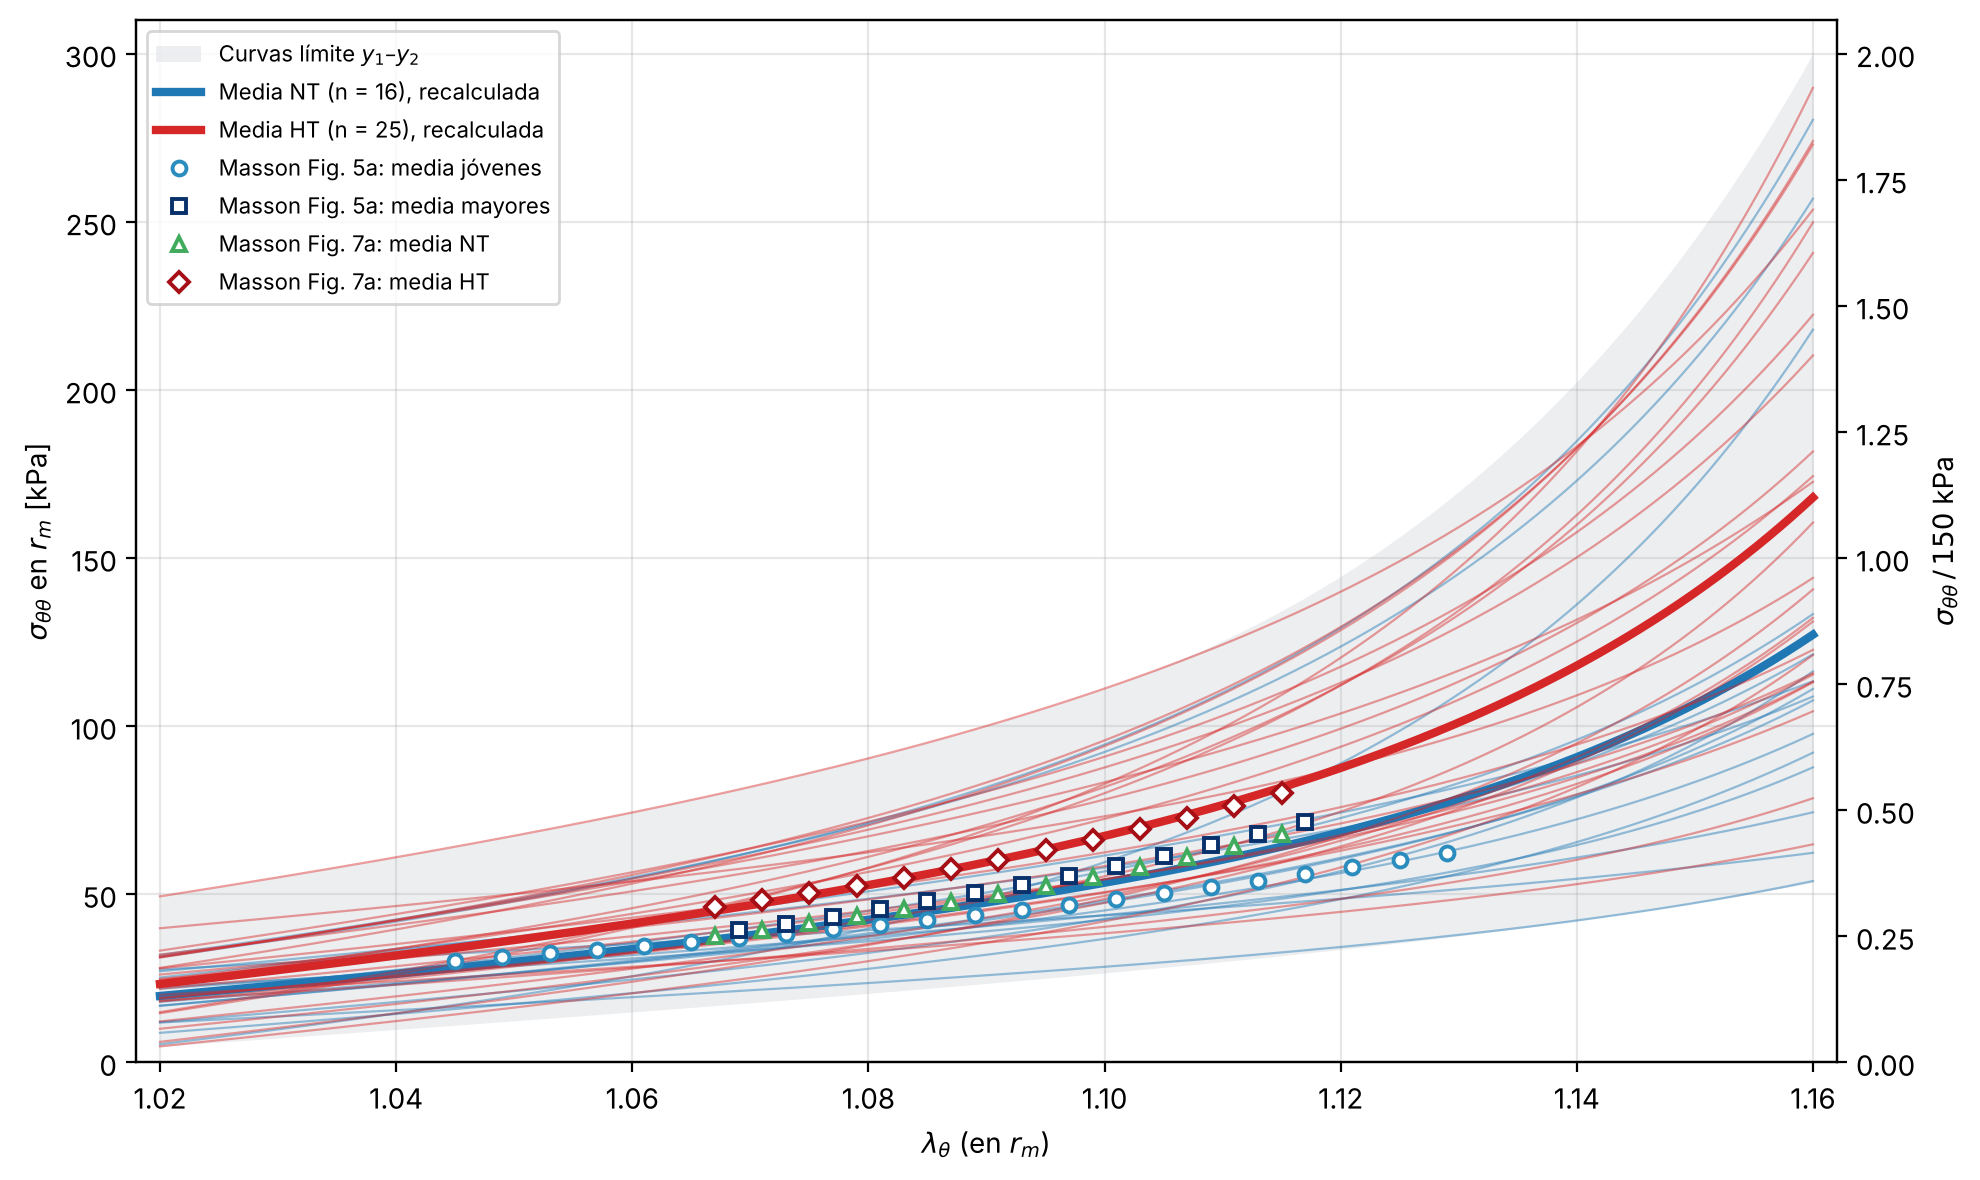
\includegraphics[width=\textwidth]{fig1_sujetos_sigma_v49.png}
\caption{The 41 subjects: circumferential stress at the media--adventitia boundary; left axis in kPa, right axis relative to 150\,kPa. Gray band: bounding curves $y_1$--$y_2$. Blue: normotensive; red: hypertensive; thick lines: recomputed means of each group. Markers: mean curves digitized from Masson et al.~\cite{masson}, Fig.~5a (young, older) and Fig.~7a (normotensive aged 39 or more, hypertensive); they cover the $\lambda_\theta$ interval shown in the original work.}\label{fig:sigma}\end{figure}

%=====================================================================
\section{Validation of the method on the stress--stretch curve}\label{sec:validacion}
\subsection{Materials: truncated lines}
One lamina of material $j$ contributes
\begin{equation}\label{eq:base}
A_j(\lambda)=S_j\,\max(0,\ \lambda-k_j):
\end{equation}
nothing up to its \emph{knot} $k_j$, and then a straight line of slope $S_j$. It idealizes a crimped fiber that bears no load until it is straightened. The graft is the sum $\sigma_{\mathrm{gr}}=\sum_j c_jA_j=A\,c$, where $c_j$ is the number of laminae of each material and $A\in\mathbb R^{999\times N}$ is the \emph{basis}. For fixed knots, the problem is linear.

\paragraph{Choice of the knots.} The knots are chosen once, for the whole population, by minimizing a function $J(k)$ that combines three requirements on the working space and the training subjects:
\begin{itemize}
\item \textbf{Accuracy: CVaR 99\,\%.} For each curve, the maximum pointwise error of the least-squares fit, $e_{\max}$ (Eq.~\ref{eq:emax}), is computed. The CVaR 99\,\% (conditional value at risk~\cite{rockafellar}) is the mean of $e_{\max}$ over the 1\,\% of curves with the largest error. A smaller term, 0.25 times the mean NRMSE, is added so that the typical fit also improves. Minimizing the mean over all curves would leave the worst ones uncontrolled; minimizing only the worst one would make the choice depend on a single curve. The CVaR lies between the two: it addresses the tail of worst curves without depending on a single one.
\item \textbf{Stability: condition number.} With the columns of $A$ scaled to a maximum of 1, the condition number is $\kappa(A)=s_{\max}/s_{\min}$, the ratio of the largest to the smallest singular value~\cite{trefethen}. It measures how much a relative error in the curve can be amplified in the amounts $c$: a 1\,\% error in $y$ can produce up to $\kappa(A)$\,\% error in $c$. If two knots are very close, their columns become similar, $s_{\min}\to0$, and the design becomes unstable (large amounts of opposite sign that cancel each other). We require $\kappa(A)<30$; the adopted bases have 28.0 (6 materials) and 19.0 (5).
\item \textbf{Sign.} The amounts of the unconstrained fit, $c=A^+y$, must be non-negative (with a tolerance of 0.01 lamina) for the 22\,500 curves of the working space, the training subjects and the bounding curves, because a negative amount of material cannot be manufactured. The function $J$ adds a penalty proportional to the negative amounts. Since the sign of $c_j$ does not depend on the slope $S_j$ (which only scales the column), this condition is determined by the knots.
\end{itemize}
The search is global, by \emph{differential evolution}~\cite{storn}: a population of candidate knot sets is improved generation after generation; each candidate is perturbed by adding the scaled difference between two others, and the result replaces the candidate if it yields a lower $J$. It requires no derivatives, which $J$ does not have (the $\max$, the sorting in the CVaR and the penalties make it non-differentiable), and it explores the whole domain, so it does not get trapped in the first local minimum. The best candidate is refined with the \emph{Nelder--Mead} simplex method~\cite{nelder}, which is also derivative-free: it moves a polytope of $N+1$ vertices through reflections, expansions and contractions until it closes in on the minimum.

\paragraph{Constraints on the knots.} Knots 2 to $N$ lie within the domain, at least 0.008 apart (if they come together, $\kappa(A)$ grows), and the last one more than 0.012 from the upper end 1.16 (otherwise its material acts on very few points and cannot be distinguished from the others). The first one, $k_1$, is sought between 0.6 and 0.98, \emph{before} the domain, for a physical reason: at $\lambda_\theta=1.02$ all arteries already carry stress (4.7 to 49\,kPa), and at that point the only material that can supply it is one that is already working. That material plays the role of elastin, which bears load in the unloaded artery. A knot $k_1<1$ means that the lamina is mounted prestretched: with $k_1=0.82$, at $\lambda=1$ it is already stretched by $1/0.82=1.22$. The upper bound 0.98 ensures that it is active over the whole domain with a margin. The lower bound, 0.6 (prestretch of 1.67), restricts the search to manufacturable values. Neither bound is active at the optimum ($k_1=0.82$ with both 5 and 6 materials): the choice does not depend on them.

\paragraph{Slopes.} $S_j=\mathrm{SLOPE}_{\max,j}/20$, where $\mathrm{SLOPE}_{\max,j}$ is the largest slope that material $j$ must supply in the working space: thus no curve requires more than 20 laminae of one material. The scale does not change the curve (what matters is $c_jS_j$), but it sets the size of one lamina.

\begin{figure}[H]\centering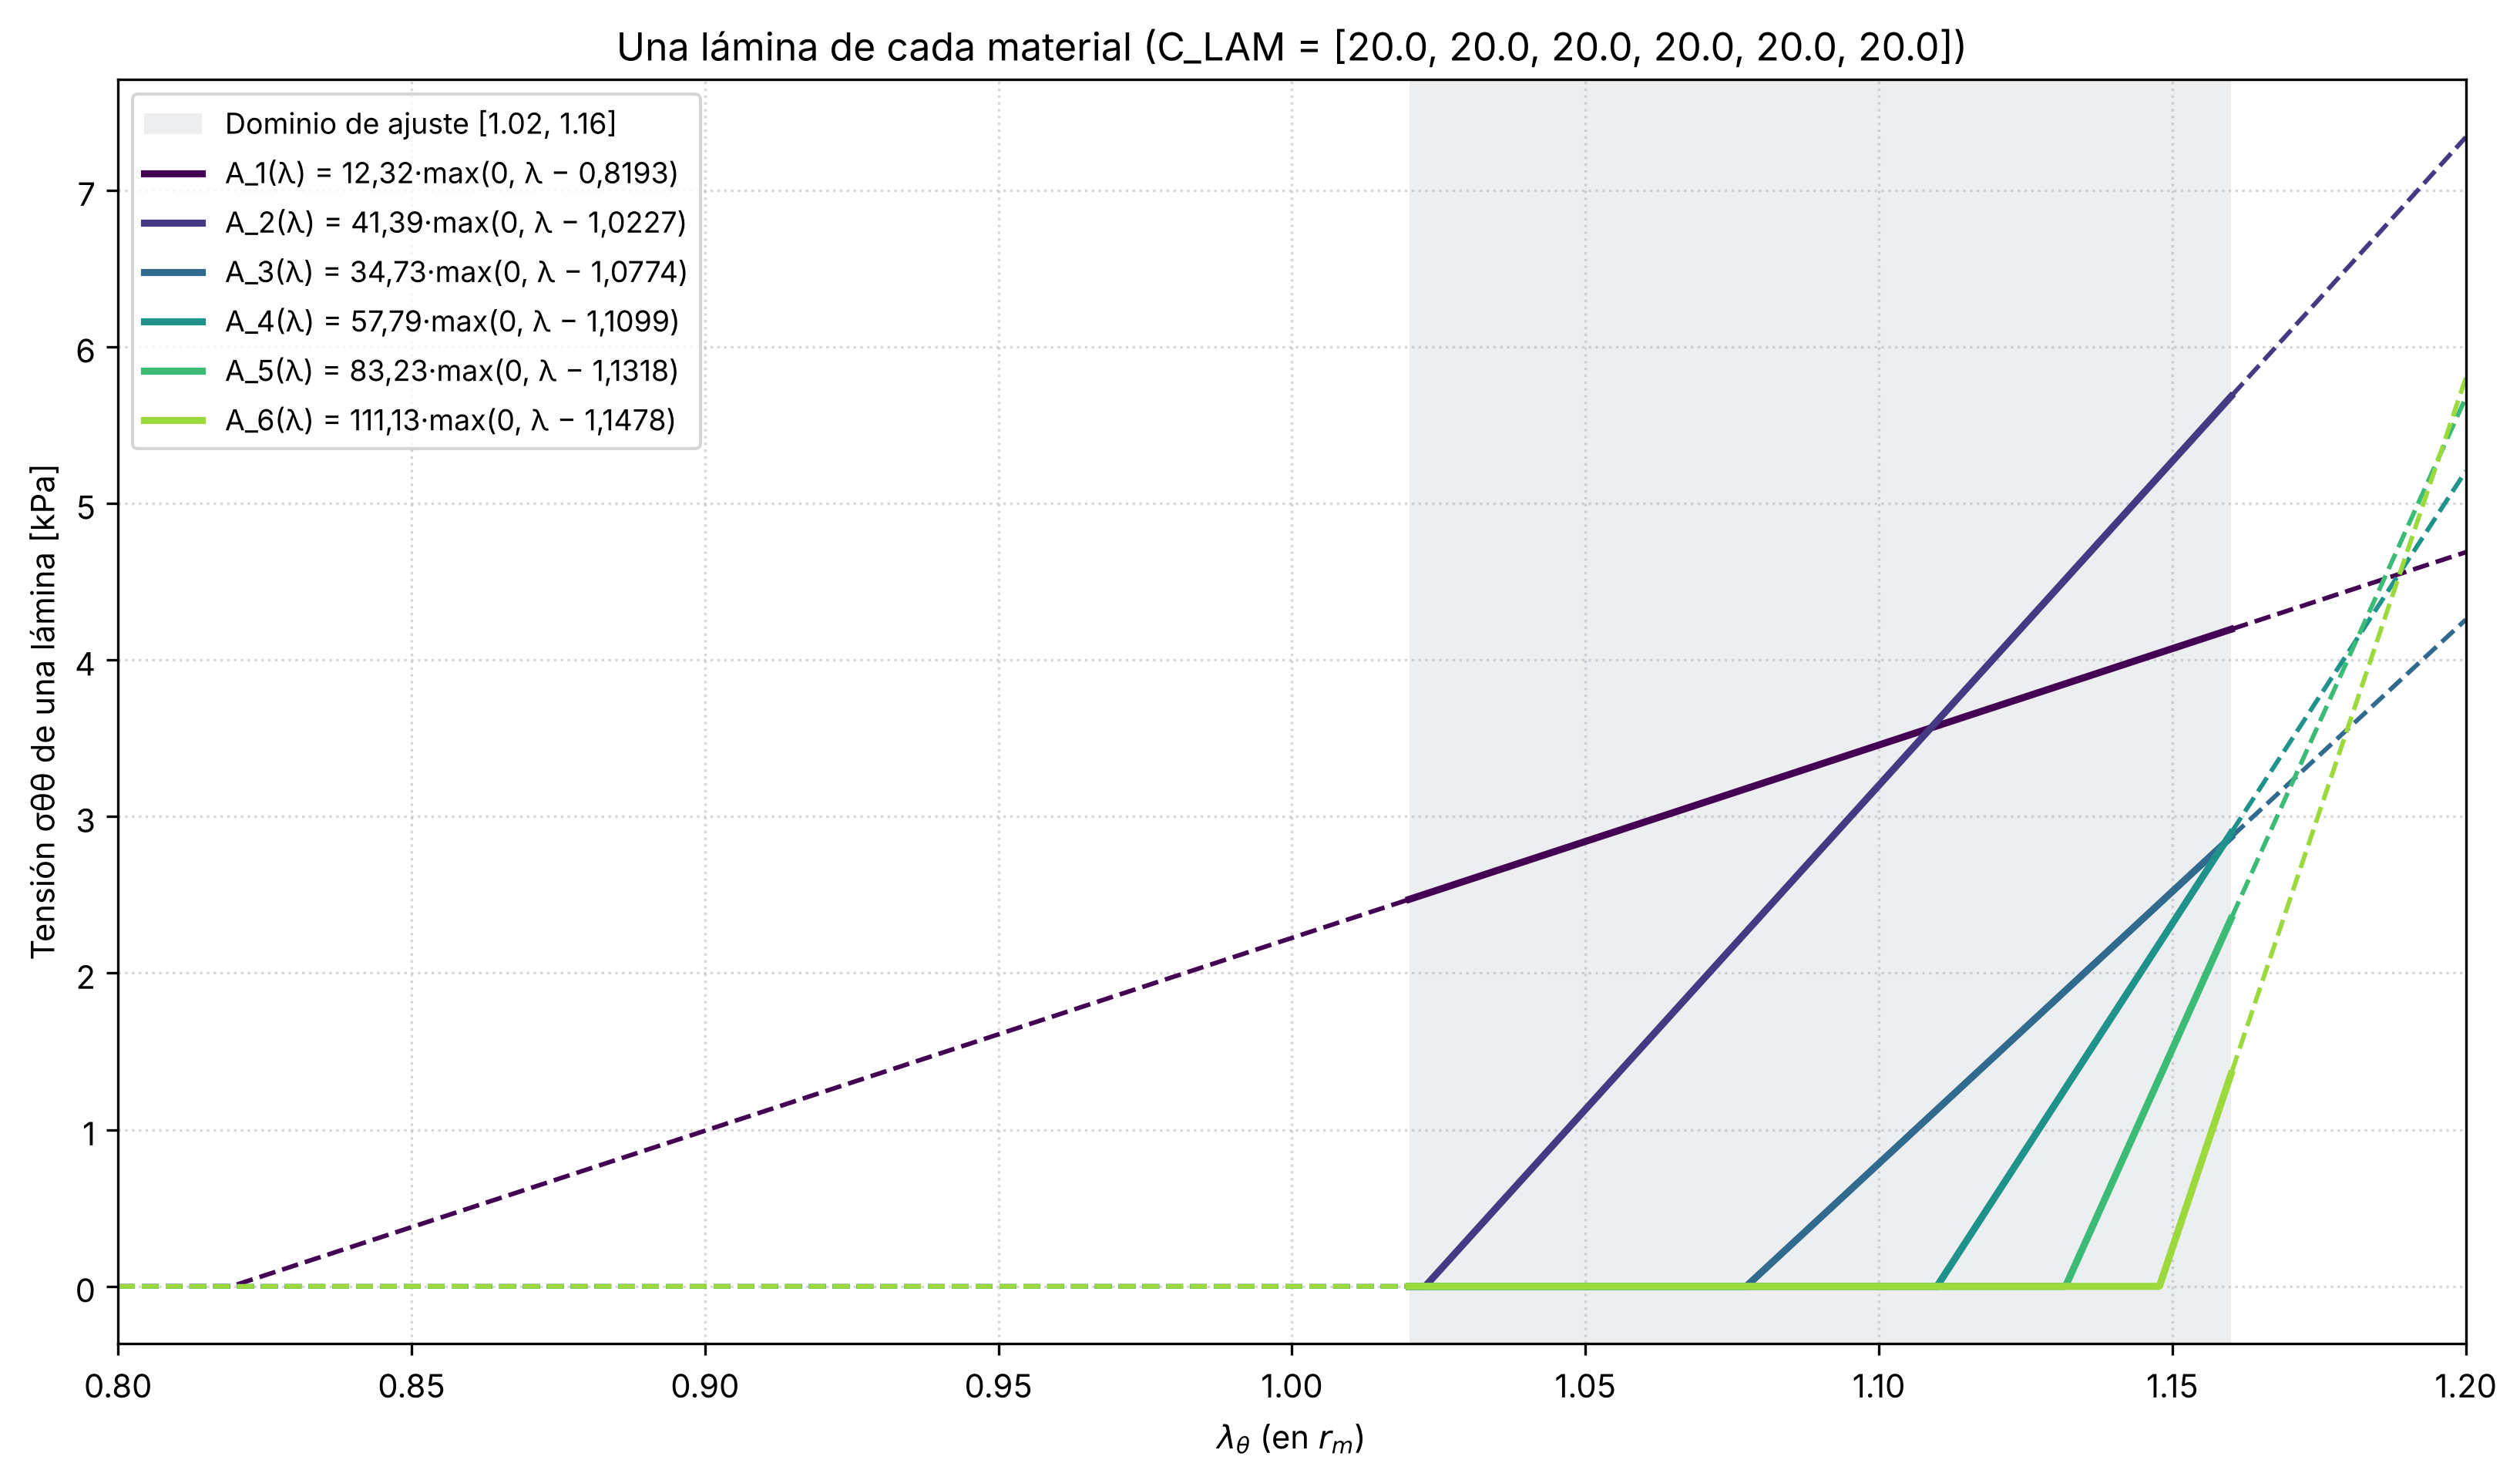
\includegraphics[width=0.85\textwidth]{bases_funcionales_v39_6.png}
\caption{The 6-material basis: one lamina of each. The first knot (0.82) lies before the domain, like elastin, which already works in the unloaded artery; the others cluster where the arterial curve bends most.}\label{fig:bases}\end{figure}

\begin{table}[H]\centering\small
\caption{Adopted bases: knots $k_j$ and slope of one lamina $S_j$ [kPa].}\label{tab:bases}
\begin{tabular}{lcccccc}\toprule
 & 1 & 2 & 3 & 4 & 5 & 6\\\midrule
6 materials, $k_j$ & 0.8193 & 1.0227 & 1.0774 & 1.1099 & 1.1318 & 1.1478\\
\phantom{6 materials, }$S_j$ & 12.32 & 41.39 & 34.73 & 57.79 & 83.23 & 111.13\\\addlinespace
5 materials, $k_j$ & 0.8228 & 1.0243 & 1.0881 & 1.1226 & 1.1447 & ---\\
\phantom{5 materials, }$S_j$ & 12.56 & 43.57 & 51.92 & 88.74 & 129.08 & ---\\\bottomrule
\end{tabular}
\end{table}

\subsection{Metric}
For a target curve $y$ with range $\Delta=\max y-\min y$,
\begin{equation}\label{eq:emax}
e_{\max}=\frac{100}{\Delta}\max_i\,|y_i-\hat y_i|\quad[\%],\qquad E_{\mathrm{rms}}=\frac{100}{\Delta}\sqrt{\frac1n\sum_i(y_i-\hat y_i)^2},
\end{equation}
where $\hat y$ is the graft curve. $e_{\max}$ is the worst point; $E_{\mathrm{rms}}$ (or NRMSE), the typical deviation. Dividing by the range makes the criterion equally demanding for a soft and a stiff artery. Target: $e_{\max}\le3$\,\%. Every design is evaluated against the original curve.

\subsection{Real-valued amounts: least squares}
With a fixed basis, the best quadratic fit is $c=A^+y$, where $A^+$ is the Moore--Penrose pseudoinverse~\cite{penrose}, computed by singular value decomposition~\cite{golub}: exact, unique and instantaneous. With the adopted knots the condition number is 19.0 (5 materials) and 28.0 (6 materials), below the threshold of 30, and no curve of the working space nor any subject requires a negative amount. The fit meets the target in all 41 subjects, with a worst error of 0.88\,\% (6 materials; median 0.67\,\%) and 1.41\,\% (5 materials; median 1.07\,\%), and in every curve of the working space.

\subsection{Integer laminae: three ways of obtaining them}
A graft is manufactured with an integer number of laminae, $z\in\mathbb Z^N_{\ge0}$. The methods fall into two classes. The first two start from a real-valued solution ---the least-squares one, $c_{\mathrm{LS}}$, or the network one, $c_{\mathrm{net}}$--- and look for integers close to it. The third does not start from any: it seeks the integers directly against the curve of the artery.
\begin{itemize}
\item \textbf{Simple:} each amount given by the network to the nearest integer.
\item \textbf{Joint (lowest $E_{\mathrm{rms}}$):} since the least-squares residual is orthogonal to the columns of $A$, $E_{\mathrm{rms}}(z)^2=E_{\mathrm{rms}}(c_{\mathrm{LS}})^2+(z-c_{\mathrm{LS}})^\top\tilde M(z-c_{\mathrm{LS}})$, with $\tilde M\propto A^\top A$ of size $N\times N$. Hence, finding the integer vector of lowest $E_{\mathrm{rms}}$ \emph{against the artery} is exactly finding the lattice point closest to $c_{\mathrm{LS}}$ in the metric $\tilde M$, which is solved exactly by tree search with Schnorr--Euchner pruning~\cite{agrell}. The optimum may lie outside the floor and ceiling of each amount. If $c_{\mathrm{LS}}$ is replaced in this search by the network output (\emph{joint from the network}), what is minimized is the distance to the curve \emph{of the network}, not to that of the artery: the result inherits the error of the network.
\item \textbf{Integer minimax design (lowest $e_{\max}$):} it does not round any real-valued solution. It directly seeks the integers that leave the narrowest tube around the curve of the artery,
\[
\min_{z,\tau}\ \tau\quad\text{s.t.}\quad -\tau\le\frac{100}{\Delta}\bigl(y_i-(Az)_i\bigr)\le\tau,\qquad z\in\mathbb Z^N_{\ge0},
\]
a mixed-integer linear program (Chebyshev approximation~\cite{cheney} with integers) solved by branch and bound with HiGHS~\cite{highs}, in about 70\,ms per curve. Its only data are the curve $y$ and the basis $A$: neither $c_{\mathrm{LS}}$ nor the network intervene, and the result is the \emph{global optimum} of that problem, the integer design with the lowest $e_{\max}$ that exists. Its result therefore does not depend on starting from the linear fit or from the network. We call it rounding only by comparison with the other two.
\end{itemize}

\begin{table}[H]\centering\small
\caption{41 subjects, integer laminae: median / worst $e_{\max}$ [\%] and subjects meeting the target. The working space is evaluated on 2000 random curves with a target of 4\,\%. All errors are measured against the original curve of the artery.}\label{tab:redondeo}
\resizebox{\textwidth}{!}{\begin{tabular}{lcccc}\toprule
& \multicolumn{2}{c}{6 materials} & \multicolumn{2}{c}{5 materials}\\\cmidrule(lr){2-3}\cmidrule(lr){4-5}
Method & 41 subjects & 2000 curves & 41 subjects & 2000 curves\\\midrule
Real-valued (least squares) & 0.67 / 0.88 · 41/41 & --- & 1.07 / 1.41 · 41/41 & ---\\
Simple (from the network) & 2.34 / 7.45 · 25/41 & 1706 & 2.23 / 7.48 · 26/41 & 1616\\
Joint from the network & 1.17 / 2.46 · 41/41 & 1998 & 1.70 / 3.56 · 40/41 & 1997\\
Joint from LS (Schnorr--Euchner) & 1.18 / 2.46 · 41/41 & 1998 & 1.70 / 3.56 · 40/41 & 1997\\
Integer minimax (MILP, against the curve) & 1.02 / 2.35 · 41/41 & 2000 & 1.47 / 3.50 · 40/41 & 2000\\\bottomrule
\end{tabular}}
\end{table}

The joint method from the network yields the same design as from least squares in 32 of the 41 subjects (6 materials) and in 35 (5 materials), and in 69 and 79\,\% of the 2000 curves; where it differs, it does so by one or two laminae, with the same worst cases, because at this level the network is very close to $c_{\mathrm{LS}}$. Neither of them, however, guarantees the lowest $e_{\max}$: for $y_1$ with 6 materials, the joint method from the network reaches 2.03\,\% and the minimax 1.10\,\% (Table~\ref{tab:redondeo3}). Each method is the best in its own measure: the joint method in $E_{\mathrm{rms}}$, the minimax in $e_{\max}$, which is the measure of the design criterion (Table~\ref{tab:redondeo}, Fig.~\ref{fig:redondeo}). Simple rounding is not advisable. With 6 materials all 41 subjects meet the target with integer laminae; with 5, one subject remains at 3.5\,\%: the limit is set by having only 5 materials, not by the method. \textbf{The minimax is adopted.}

\begin{figure}[H]\centering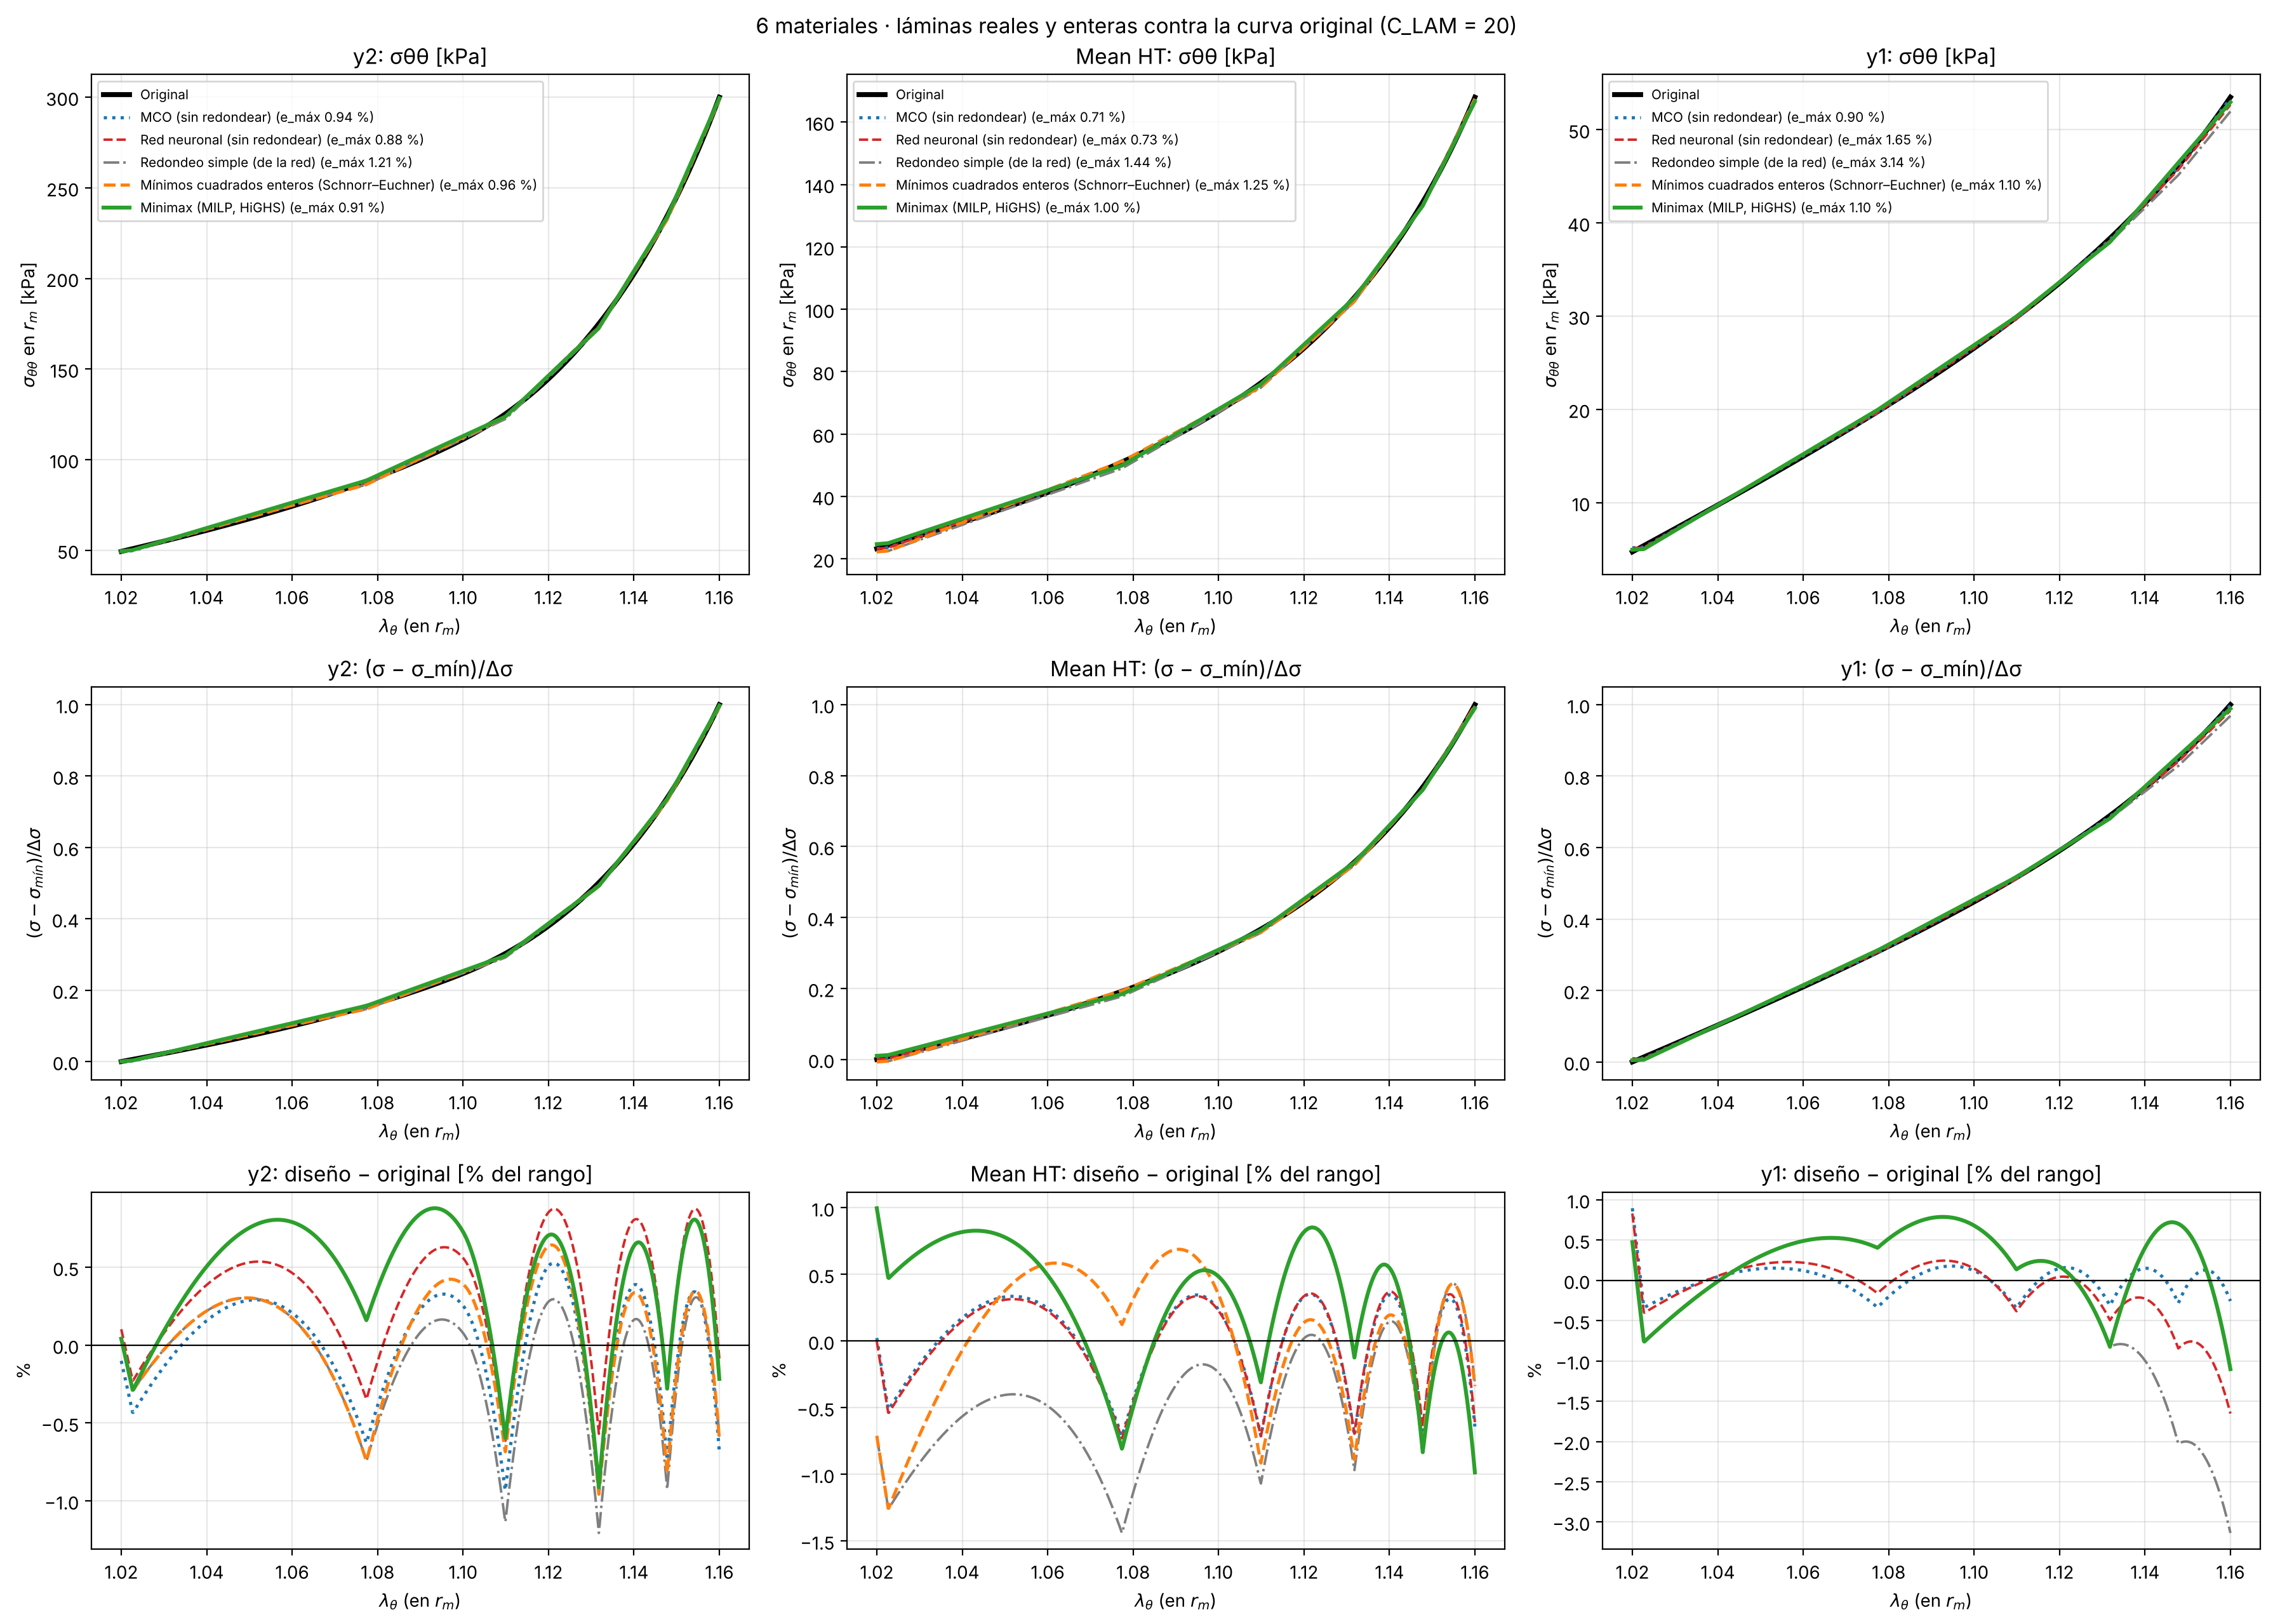
\includegraphics[width=\textwidth]{redondeo_y2_meanHT_y1_v39_6.png}
\caption{6 materials: the stiffest curve of the band ($y_2$), the hypertensive mean and the softest curve ($y_1$). Top: stress; middle: dimensionless form; bottom: design $-$ original in \% of the range. The minimax (green) distributes the error so that the worst point is as small as possible.}\label{fig:redondeo}\end{figure}
\begin{table}[H]\centering\small
\caption{Designs of Fig.~\ref{fig:redondeo} (6 materials): laminae of each material $c_j$ (real-valued in the first two rows of each curve, integer in the others) and errors against the original curve, $E_{\mathrm{rms}}$ and $e_{\max}$ [\% of the range].}\label{tab:redondeo3}
\begin{tabular}{llcccccccc}\toprule
Curve & Method & $c_1$ & $c_2$ & $c_3$ & $c_4$ & $c_5$ & $c_6$ & $E_{\mathrm{rms}}$ & $e_{\max}$\\\midrule
$y_2$ & Least squares (real-valued) & 19.86 & 10.33 & 12.85 & 20.00 & 17.78 & 14.58 & 0.32 & 0.94\\
 & Neural network (real-valued) & 20.06 & 10.35 & 12.83 & 20.07 & 17.85 & 14.73 & 0.46 & 0.88\\
 & Simple rounding (of the network) & 20 & 10 & 13 & 20 & 18 & 15 & 0.36 & 1.21\\
 & Joint (Schnorr--Euchner) & 20 & 10 & 14 & 19 & 18 & 15 & 0.34 & 0.96\\
 & Minimax (MILP) & 20 & 11 & 11 & 20 & 19 & 14 & 0.56 & 0.91\\
\addlinespace
HT mean & Least squares (real-valued) & 9.43 & 8.86 & 8.54 & 8.17 & 7.96 & 7.59 & 0.30 & 0.71\\
 & Neural network (real-valued) & 9.41 & 8.87 & 8.55 & 8.18 & 7.96 & 7.58 & 0.30 & 0.73\\
 & Simple rounding (of the network) & 9 & 9 & 9 & 8 & 8 & 8 & 0.64 & 1.44\\
 & Joint (Schnorr--Euchner) & 9 & 10 & 6 & 9 & 8 & 8 & 0.49 & 1.25\\
 & Minimax (MILP) & 10 & 8 & 10 & 8 & 7 & 8 & 0.54 & 1.00\\
\addlinespace
$y_1$ & Least squares (real-valued) & 2.08 & 5.72 & 1.41 & 1.32 & 1.18 & 1.07 & 0.16 & 0.90\\
 & Neural network (real-valued) & 2.07 & 5.78 & 1.26 & 1.32 & 1.08 & 0.87 & 0.37 & 1.65\\
 & Simple rounding (of the network) & 2 & 6 & 1 & 1 & 1 & 1 & 0.91 & 3.14\\
 & Joint (Schnorr--Euchner) & 2 & 6 & 1 & 1 & 2 & 0 & 0.49 & 1.10\\
 & Minimax (MILP) & 2 & 6 & 1 & 1 & 2 & 0 & 0.49 & 1.10\\
\bottomrule
\end{tabular}
\end{table}

\clearpage
\subsection{The neural network}
A neural network receives the curve and returns the amount of each material in a single evaluation: it learns the map $y\mapsto A^+y$ for the class of J-shaped curves.

\paragraph{Data.} 50\,000 curves in seven families: basis curves (sums of one or several laminae of the basis itself, 40\,\%), which teach what each material does on its own, and physiological curves (60\,\%): Masson's law mixed, perturbed or sampled (the three families of the working space), another four-parameter exponential law fitted to the subjects, and the training subjects. The input carries 1\,\% Gaussian noise; the label is the fit of the clean curve. Stratified split: 35\,000 for training, 5000 for validation and 10\,000 for testing.

\paragraph{Architecture and training.} Multilayer perceptron~\cite{goodfellow} $999\to256\to128\to64\to N$ (Fig.~\ref{fig:red}), with standardized input $\log(y+22)$, ReLU~\cite{relu}, layer normalization~\cite{layernorm} and L2 regularization ($10^{-5}$); about 298\,000 parameters. Loss: squared error of the amounts, plus 5 times the error of the reconstructed curve, plus 5 times the amount assigned to materials absent from the basis curves (\emph{crosstalk}). Adam~\cite{adam} with gradient clipping, batches of 256, learning-rate reduction on plateau and early stopping~\cite{prechelt}; TensorFlow/Keras~\cite{tf}. The learning curves and training metrics are given in Appendix~\ref{sec:entrenamiento}.

\begin{figure}[H]\centering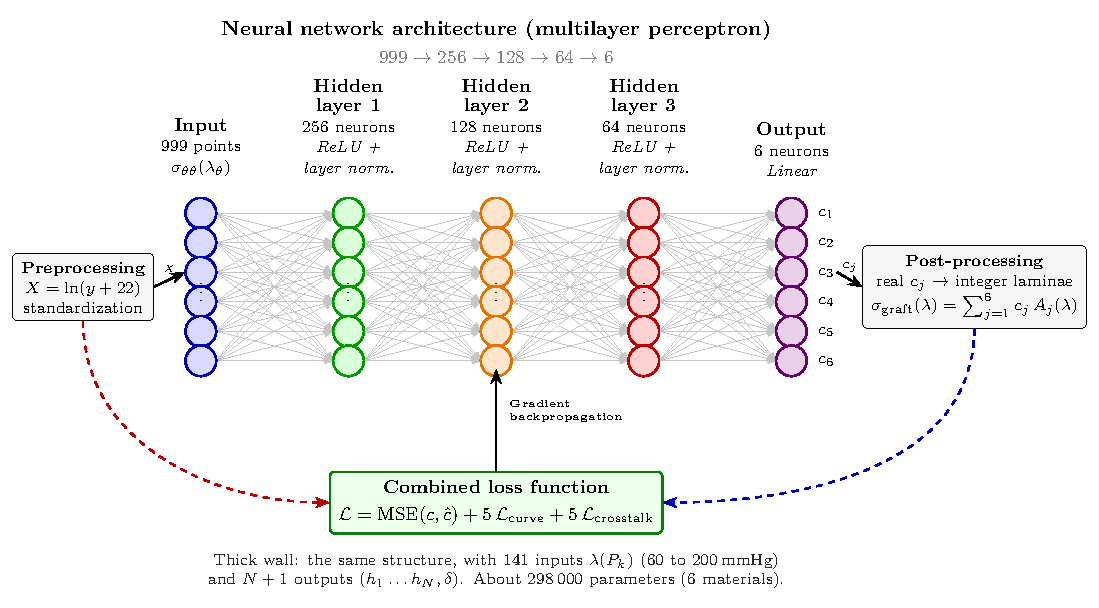
\includegraphics[width=\textwidth]{red_neuronal_en.pdf}
\caption{Schematic of the neural network for 6 materials. The input is the 999 points of the artery curve $\sigma_{\theta\theta}(\lambda_\theta)$; three hidden layers (256, 128 and 64 neurons, ReLU and layer normalization) lead to 6 linear outputs, the real-valued numbers $c_1\ldots c_6$ of laminae of each material, which are then rounded to integer laminae. The loss combines the error in $c$, the error of the graft curve $\sum_j c_j A_j$ and the \emph{crosstalk} (dashed lines); its gradient is backpropagated to update the weights. Only some neurons of each layer are drawn. For the thick wall the same structure is used with 141 inputs $\lambda(P_k)$ and $N+1$ outputs $(h_1\ldots h_N,\delta)$.}\label{fig:red}
\end{figure}

\paragraph{Class check.} Before the network is used, it is verified that the curve admits a non-negative approximation with 40 truncated lines (NRMSE $\le2$\,\%), by non-negative least squares~\cite{lawson}. A curve that does not admit it is not J-shaped and cannot be reproduced with layers.

\paragraph{Results.} In the 41 subjects the network meets the target in every case, with an NRMSE barely above the optimum (mean excess of +3.1\,\% with 6 materials and +1.6\,\% with 5; worst $e_{\max}$ 1.11 and 1.38\,\%). On the 10\,000 test curves, the physiological families lie between +1.0 and +3.1\,\% of the optimum, and the network meets the target in 99.9 to 100\,\% of each family (Table~\ref{tab:familias}). One least-squares step applied to the network output (polishing) yields the exact optimum. The network takes 0.06\,ms per curve in batch mode, the same as the linear fit.

\begin{table}[H]\centering\small
\caption{Network versus exact fit on the 10\,000 test curves (with 1\,\% input noise), by family. $n$: curves in the family. Excess: $\overline{\mathrm{NRMSE}}_{\mathrm{net}}/\overline{\mathrm{NRMSE}}_{\mathrm{LS}}-1$, with the NRMSE averaged over the curves of the family (0\,\% would mean matching the exact fit). Meets: percentage of curves for which the network design has $e_{\max}\le3$\,\%. The exact fit meets the target in all of them.}\label{tab:familias}
\begin{tabular}{lrcccc}\toprule
 & & \multicolumn{2}{c}{6 materials} & \multicolumn{2}{c}{5 materials}\\\cmidrule(lr){3-4}\cmidrule(lr){5-6}
Family & $n$ & excess & meets & excess & meets\\\midrule
Masson, mixing and small perturbation & 2000 & +1.2\,\% & 100\,\% & +0.6\,\% & 100\,\%\\
Masson, wide mixing and extrapolation & 1500 & +1.7\,\% & 100\,\% & +1.1\,\% & 100\,\%\\
Masson, uniform parameters & 1000 & +1.7\,\% & 100\,\% & +0.7\,\% & 100\,\%\\
Another exponential law & 1000 & +3.1\,\% & 99.9\,\% & +1.7\,\% & 99.8\,\%\\
Training subjects & 500 & +1.0\,\% & 100\,\% & +0.3\,\% & 100\,\%\\
Basis curves, one material & 2000 & +30.6\,\% & 99.95\,\% & +17.4\,\% & 100\,\%\\
Basis curves, combined & 2000 & +54.6\,\% & 98.5\,\% & +33.1\,\% & 99.6\,\%\\\bottomrule
\end{tabular}
\end{table}
The rows are the seven families of the data set. The first three are curves of Masson's law: with parameters of 2 to 4 training subjects mixed and slightly perturbed; mixed with weights that allow some departure from the range of the subjects (extrapolation); or drawn uniformly between the minimum and maximum of each parameter. ``Another exponential law'' is a four-parameter law different from Masson's, fitted to the subjects. ``Training subjects'' are the 31 subjects with noise. The last two are sums of laminae of the basis itself: of a single material or of several. For them the relative excess is high because the optimum is nearly zero (the curve \emph{is} an exact combination of the basis): they are low-stress polygonal curves that do not represent arteries, and they serve to teach the network what each material does on its own.

\paragraph{A law never seen.} We generated 300 curves of a Fung-type exponential law~\cite{fung}, $\sigma=C+a\bigl(e^{b(\lambda-\lambda_{\min})}-1\bigr)$, with parameters mixed from fits to the training subjects and 1\,\% noise; this law is not part of the training. The network reproduces them with an excess of +4.6\,\% (6 materials) and +2.8\,\% (5) over the optimum, with $R^2\ge0.996$, and all of them admit a design without negative amounts. The class check accepts 100\,\% of the Fung curves and of the subjects, and rejects 98\,\% of the curves that lose their J shape when modulated with an oscillation.

\paragraph{Does the network improve on the exact method?} Three variants were tested. (a) Trained directly on the reconstructed curve, without labels, the network reaches the same fit (median $E_{\mathrm{rms}}$ 0.284 versus 0.280\,\% with 6 materials). (b) Trained with integer laminae as labels, it still outputs non-integer numbers and its worst cases become worse. (c) As a smoother of measured curves, before the minimax, it performs practically the same as the linear fit (6 materials, 3\,\% noise: worst error 2.90 versus 3.84\,\%; with 5 materials, 5.31 versus 4.59\,\%). What does matter with noise is not to apply the minimax to the measured curve, which it follows noise included (median 3.86\,\% with 3\,\% noise), but to the fitted curve (1.38\,\%).

\subsection{External validation: measurements by other authors}\label{sec:externa}
To verify that the method does not depend on the artery with which it was built, it was applied to $\sigma_{\theta\theta}(\lambda_\theta)$ curves from four independent studies, with other constitutive laws, other arteries, isolated layers, another species and in vivo measurements. \textbf{Nothing was changed}: the same knots and slopes (Table~\ref{tab:bases}), the same network, the same class check and the same minimax.

\paragraph{Curves.} Each curve is recomputed with the published parameters:
\begin{itemize}
\item \textbf{Sommer and Holzapfel}~\cite{sommer} (Tables 1 and 2): 39 human specimens of common (CCA) and internal (ICA) carotid arteries, tested by extension--inflation: intact wall (21), adventitia (13, 33\,kPa domain) and media--intima (7). Holzapfel law with fiber dispersion, $\Psi=\tfrac{\mu}{2}(I_1-3)+\tfrac{k_1}{k_2}\bigl(e^{Q}-1\bigr)$, $Q=k_2\bigl[(1-\rho)(I_1-3)^2+\rho(I_4-1)^2\bigr]$; we use $\sigma_{\theta\theta}-\sigma_{rr}$ with $\lambda_z=1.10$, the in vivo value adopted by the authors.
\item \textbf{Holzapfel et al.}~\cite{holzapfel}: rabbit carotid artery, media and adventitia, HGO law with two fiber families at $\pm\beta$, $\lambda_z=1.10$.
\item \textbf{Liu et al.}~\cite{liu} (Table 1): 12 human carotid arteries with plaque, characterized in vivo by magnetic resonance; modified Mooney--Rivlin law in uniaxial tension, $\sigma=2\lambda(\lambda-\lambda^{-2})\bigl(c_1+D_1D_2e^{D_2(\lambda^2+2/\lambda-3)}\bigr)$.
\item \textbf{Kamenskiy et al.}~\cite{kamenskiy}: 16 patients, common, external (ECA) and internal carotid arteries measured in vivo over the cardiac cycle (48 curves). For each artery they report the stress and the tangent modulus at diastole and systole, and the diameters; with these four numbers we build $\sigma(\varepsilon)=\sigma_d+\alpha\bigl(e^{\beta\varepsilon}-1\bigr)$ on $\varepsilon\in[0,\varepsilon_s]$, with $\sigma(\varepsilon_s)=\sigma_s$ exactly and $\beta$ reproducing both slopes. In all 48, the systolic slope exceeds the diastolic one: all are J-shaped.
\end{itemize}

\paragraph{Mapping to the design domain.} Each curve lives in its own range of $\lambda$. It is mapped to $[1.02,\,1.16]$ by an affine change of $\lambda$, leaving the stress unchanged. This change is equivalent to what the real graft allows: a prestretch (shift of the knots, the $\delta$ of Section~\ref{sec:aplicacion}) and the choice of the reference radius (scale). Two protocols:
\begin{itemize}
\item \textbf{T (stress window):} the window of $\lambda$ in which the law spans the stresses of the Masson population at the ends of the domain; the median and the four combinations of quartiles are used (5 windows per curve). For the complete laws (Sommer, Holzapfel, Liu).
\item \textbf{M (measured window):} the diastole--systole interval measured in vivo, with its actual stresses (Liu, Kamenskiy).
\end{itemize}
In total, 327 curves (Fig.~\ref{fig:ext}).

\begin{figure}[H]\centering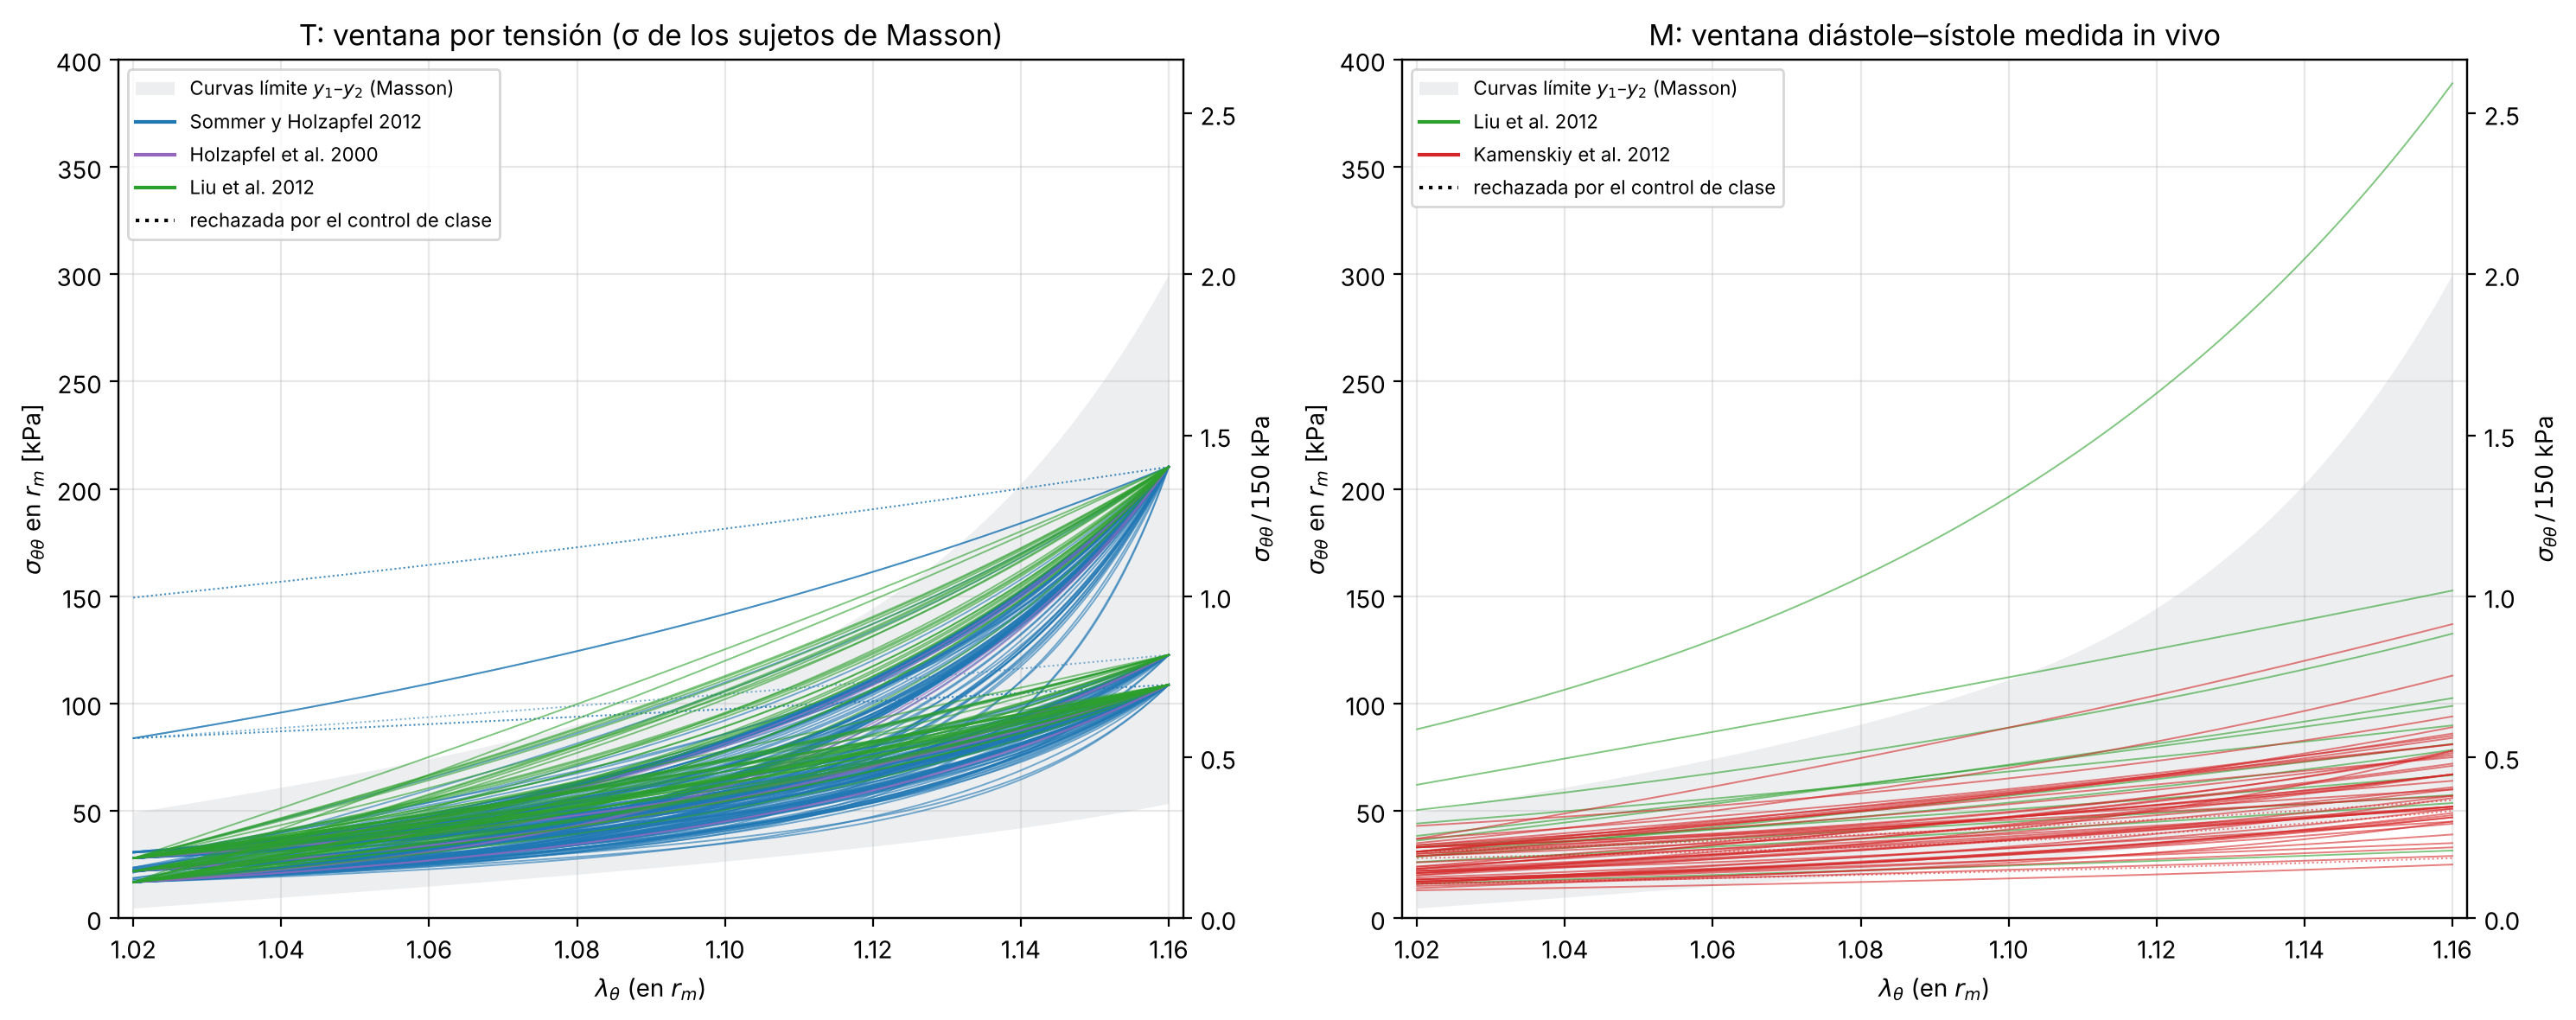
\includegraphics[width=\textwidth]{v49_curvas_externas_6.png}
\caption{The 327 external curves in the design domain, with the scales of Fig.~\ref{fig:sigma}: left axis in kPa, right axis relative to 150\,kPa (here up to 400\,kPa, because one curve of Liu et al.\ reaches 389\,kPa). Left: protocol T; right: protocol M. Gray band: bounding curves $y_1$--$y_2$ of the Masson population. Dotted: rejected by the class check.}\label{fig:ext}\end{figure}

\paragraph{Results.} Table~\ref{tab:ext} summarizes, by study and specimen type, the curves accepted by the class check.
\begin{table}[H]\centering\small
\caption{External validation (accepted / total curves). For each number of materials: worst $e_{\max}$ of the least-squares fit [\%]; curves meeting the 3\,\% target with integer laminae (minimax) and their worst $e_{\max}$ [\%]; curves for which the network meets the target.}\label{tab:ext}
\resizebox{\textwidth}{!}{%
\begin{tabular}{lllc|cccc|cccc}\toprule
 & & & & \multicolumn{4}{c|}{6 materials} & \multicolumn{4}{c}{5 materials}\\
Study & Specimen & Prot. & Accepted & LS worst & Integer $\le3$\,\% & Integer worst & Net $\le3$\,\% & LS worst & Integer $\le3$\,\% & Integer worst & Net $\le3$\,\%\\\midrule
Sommer and Holzapfel~\cite{sommer} & CCA adventitia & T & 27/30 & 2.83 & 27/27 & 2.03 & 24/27 & 4.16 & 27/27 & 2.89 & 24/27\\
 & CCA media-intima & T & 20/20 & 0.99 & 20/20 & 2.11 & 20/20 & 1.54 & 20/20 & 2.22 & 20/20\\
 & CCA wall & T & 55/55 & 2.66 & 55/55 & 1.93 & 54/55 & 3.91 & 55/55 & 2.70 & 53/55\\
 & ICA adventitia & T & 25/27 & 1.16 & 25/25 & 1.86 & 25/25 & 1.83 & 25/25 & 2.62 & 25/25\\
 & ICA media-intima & T & 15/15 & 1.13 & 15/15 & 1.65 & 15/15 & 1.76 & 15/15 & 2.54 & 15/15\\
 & ICA wall & T & 50/50 & 1.54 & 50/50 & 1.96 & 50/50 & 2.28 & 50/50 & 2.50 & 49/50\\
Holzapfel et al.~\cite{holzapfel} & rabbit adventitia & T & 5/5 & 1.16 & 5/5 & 1.94 & 5/5 & 1.80 & 5/5 & 2.15 & 5/5\\
 & rabbit media & T & 5/5 & 1.13 & 5/5 & 1.85 & 5/5 & 1.75 & 5/5 & 2.25 & 5/5\\
Liu et al.~\cite{liu} & carotid with plaque & M & 12/12 & 1.06 & 8/12 & 8.09 & 10/12 & 1.59 & 8/12 & 8.16 & 10/12\\
 & carotid with plaque & T & 60/60 & 1.41 & 60/60 & 2.15 & 58/60 & 2.18 & 60/60 & 2.21 & 60/60\\
Kamenskiy et al.~\cite{kamenskiy} & CCA & M & 16/16 & 1.28 & 11/16 & 4.57 & 16/16 & 1.84 & 8/16 & 5.21 & 16/16\\
 & ECA & M & 14/16 & 1.19 & 9/14 & 8.69 & 14/14 & 1.78 & 7/14 & 9.67 & 14/14\\
 & ICA & M & 15/16 & 1.03 & 10/15 & 6.60 & 14/15 & 1.53 & 7/15 & 6.98 & 14/15\\
\bottomrule
\end{tabular}}
\end{table}

\begin{figure}[H]\centering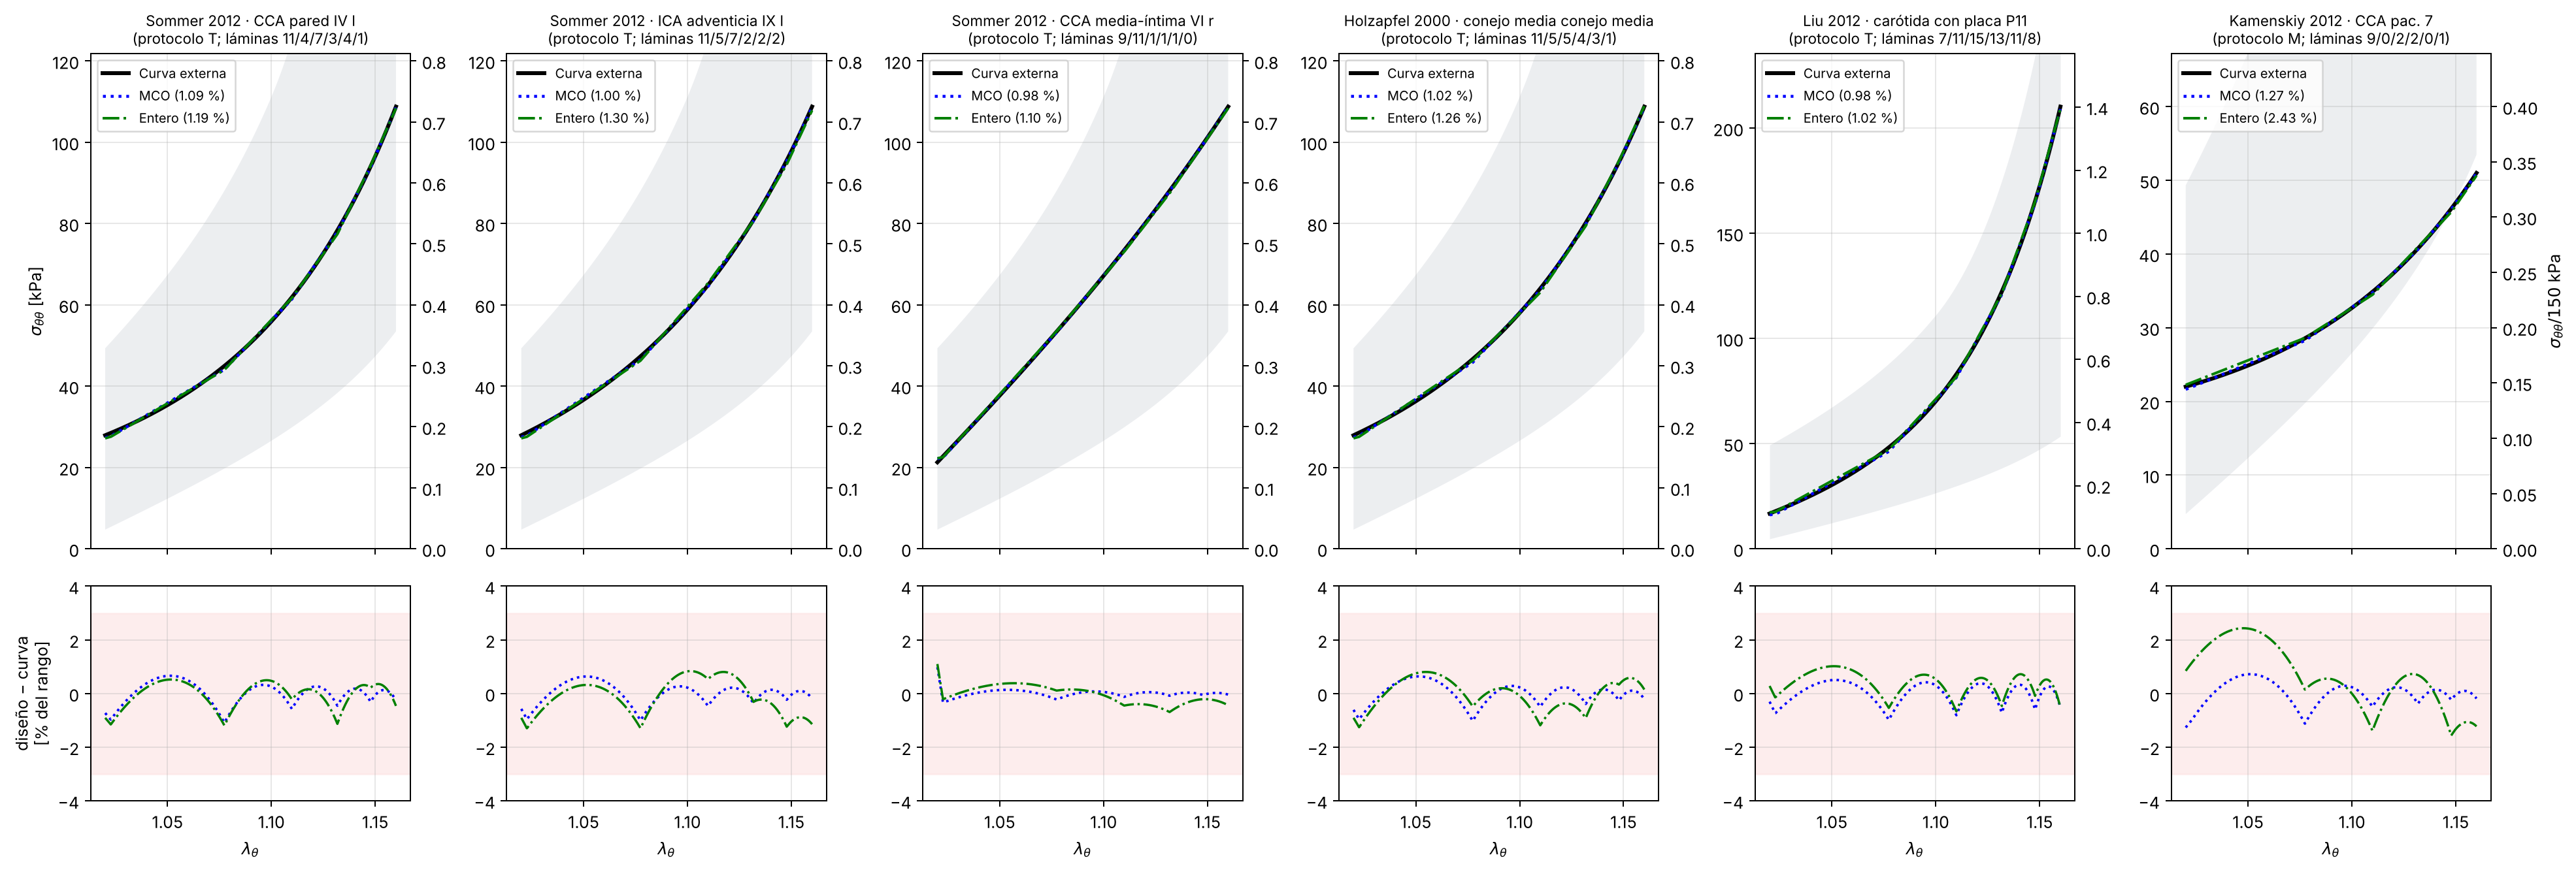
\includegraphics[width=\textwidth]{v49_representativas_6.png}
\caption{Representative curves, 6 materials: the median case of the integer design for each study. Top: external curve (black), least squares (blue) and integer laminae by minimax (green), with the worst error in parentheses and the laminae of each material in the title; right axis, stress relative to 150\,kPa. Bottom: design $-$ curve in \% of the range (band: $\pm3$\,\% target).}\label{fig:rep}\end{figure}
\begin{table}[H]\centering\small
\caption{Representative curves of Figs.~\ref{fig:ext} and~\ref{fig:rep} (6 materials): laminae of each material by least squares (real-valued) and by minimax (integer), with $E_{\mathrm{rms}}$ and $e_{\max}$ [\% of the range]. All 327 curves, with their laminae and errors, are provided in the supplementary material.}\label{tab:rep}
\resizebox{\textwidth}{!}{%
\begin{tabular}{llcccccccc}\toprule
Study · specimen · curve & Fit & $c_1$ & $c_2$ & $c_3$ & $c_4$ & $c_5$ & $c_6$ & $E_{\mathrm{rms}}$ & $e_{\max}$\\\midrule
\multirow{2}{*}{Sommer--Holzapfel · CCA wall · IV l} & Least squares & 11.06 & 3.95 & 6.70 & 3.86 & 2.81 & 1.99 & 0.41 & 1.09\\
 & Integer minimax & 11 & 4 & 7 & 3 & 4 & 1 & 0.47 & 1.19\\
\addlinespace
\multirow{2}{*}{Sommer--Holzapfel · ICA adventitia · IX l} & Least squares & 11.11 & 4.95 & 6.09 & 3.17 & 2.22 & 1.49 & 0.38 & 1.00\\
 & Integer minimax & 11 & 5 & 7 & 2 & 2 & 2 & 0.65 & 1.30\\
\addlinespace
\multirow{2}{*}{Sommer--Holzapfel · CCA media--intima · VI r} & Least squares & 8.96 & 10.93 & 1.61 & 0.89 & 0.57 & 0.38 & 0.12 & 0.98\\
 & Integer minimax & 9 & 11 & 1 & 1 & 1 & 0 & 0.32 & 1.10\\
\addlinespace
\multirow{2}{*}{Holzapfel et al. · rabbit, media} & Least squares & 11.10 & 4.67 & 6.24 & 3.37 & 2.40 & 1.65 & 0.38 & 1.02\\
 & Integer minimax & 11 & 5 & 5 & 4 & 3 & 1 & 0.55 & 1.26\\
\addlinespace
\multirow{2}{*}{Liu et al. · carotid with plaque · P11} & Least squares & 6.54 & 11.26 & 15.37 & 12.52 & 10.74 & 9.02 & 0.38 & 0.98\\
 & Integer minimax & 7 & 11 & 15 & 13 & 11 & 8 & 0.55 & 1.02\\
\addlinespace
\multirow{2}{*}{Kamenskiy et al. · CCA (in vivo, M) · pat. 7} & Least squares & 8.75 & 0.19 & 2.42 & 1.21 & 0.84 & 0.55 & 0.43 & 1.27\\
 & Integer minimax & 9 & 0 & 2 & 2 & 0 & 1 & 1.33 & 2.43\\
\bottomrule
\end{tabular}}
\end{table}

\begin{figure}[H]\centering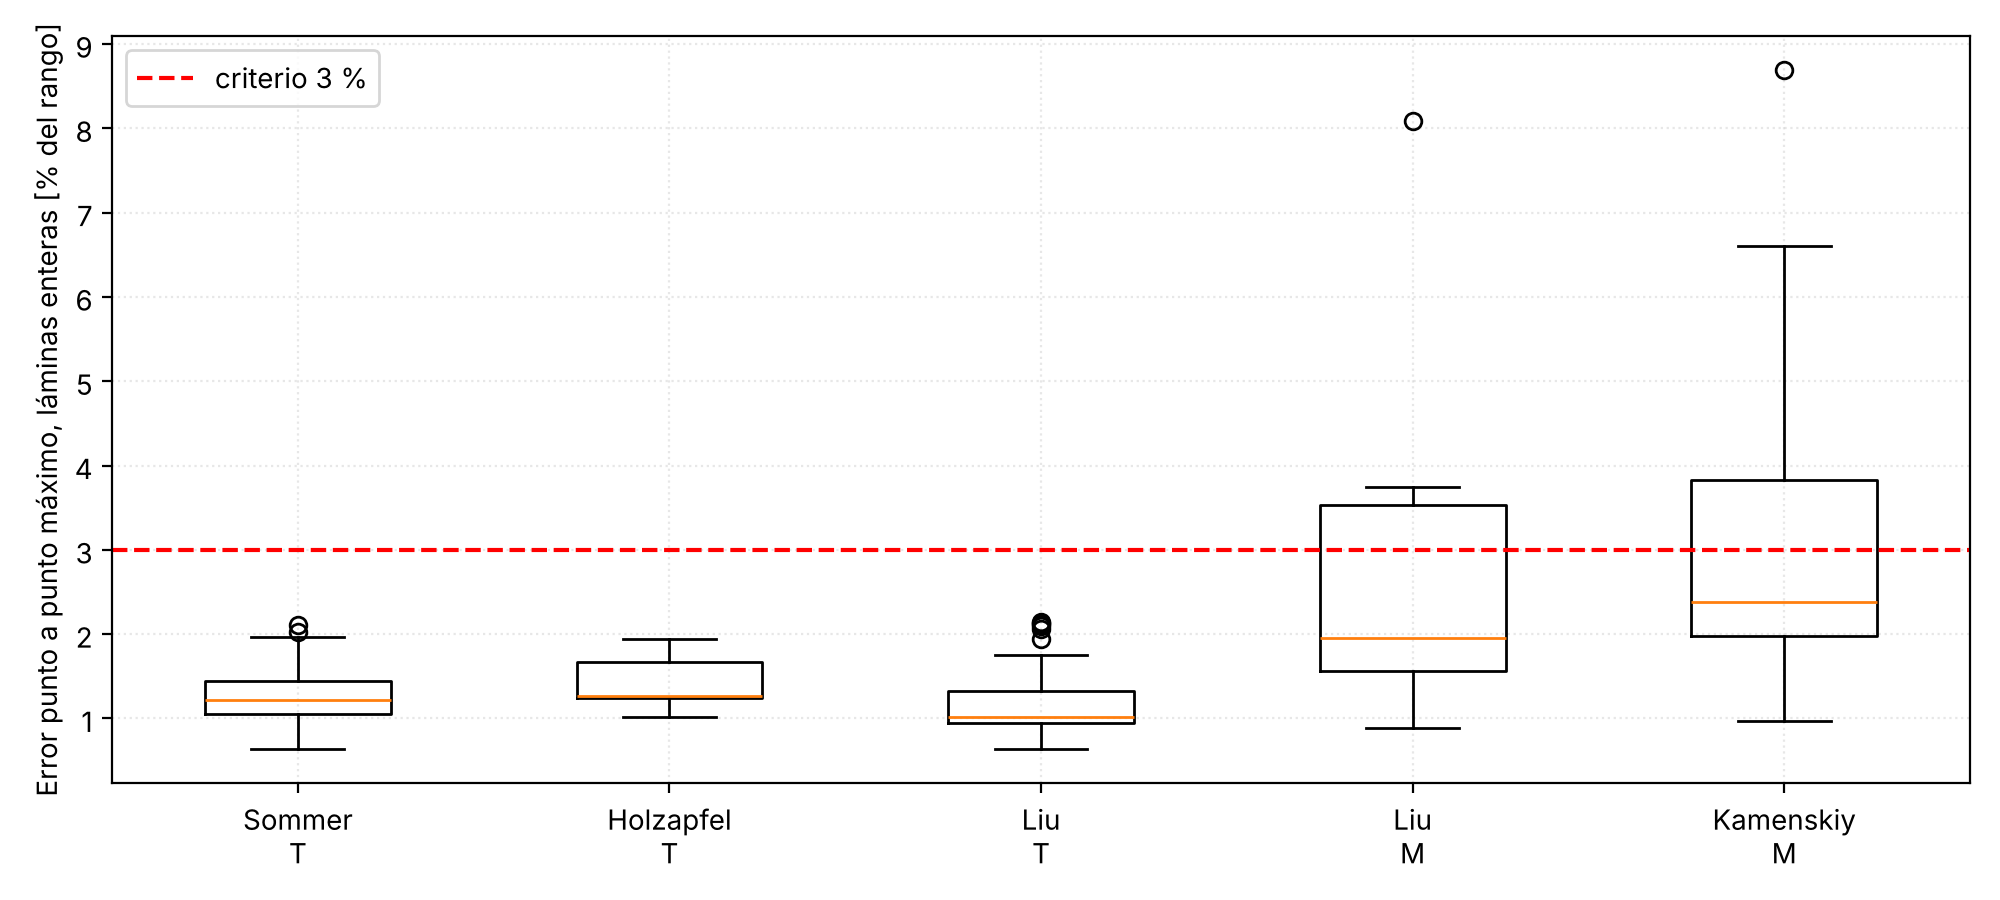
\includegraphics[width=0.85\textwidth]{v49_error_entero_6.png}
\caption{Worst error of the integer design by study and protocol, 6 materials (accepted curves). Red line: 3\,\% target.}\label{fig:boxext}\end{figure}

\begin{enumerate}[label=(\roman*)]
\item \textbf{The basis suffices.} With 6 materials, no accepted curve exceeds 2.83\,\% with least squares. With 5, two curves (one CCA wall and one CCA adventitia) slightly exceed the target with real-valued amounts (3.91 and 4.16\,\%), but the integer minimax brings them to 2.70 and 2.89\,\%: the minimax controls the worst point and least squares does not.
\item \textbf{Integer laminae.} At physiological stresses (protocol T) all 262 curves meet the target, with both 6 and 5 materials (worst 2.15 and 2.89\,\%; Figs.~\ref{fig:rep} and~\ref{fig:boxext}). In the in vivo windows (M), 38 of 57 meet it (6 materials) and 30 of 57 (5). Those that fail are the ones with a small stress excursion (12 to 30\,kPa, versus about 100\,kPa in T): one lamina of the first material shifts the curve by a few kPa, which is many percent of that range. In kPa, the worst integer error in M is 2.7\,kPa. With laminae of half the thickness ---a sensitivity analysis, without changing the adopted criterion--- 54 of 57 meet it (6 materials) and 52 of 57 (5). The limit is set by the lamina thickness, not by the basis or the method.
\item \textbf{The network.} Its median worst error is 1\,\% in all studies. Within the $y_1$--$y_2$ band it meets the target in 288 of 290 curves (6 materials) and 286 of 290 (5), although none of these laws is part of its training. Outside the band it degrades (22 of 29): for Liu P11, with stresses from 88 to 389\,kPa, above $y_2$, the network errs by 25\,\%, whereas least squares and the minimax give 1.1 and 0.9\,\%. This confirms the role of the network: a fast start within the trained space; the final design is given by the minimax, which does not depend on the band.
\item \textbf{The class check.} It rejected 8 of the 327 curves: five windows of the VIII\,r adventitias, which with $\lambda_z=1.10$ already exceed the requested stress at $\lambda=1$ and have no soft initial segment, and three very short in vivo windows of Kamenskiy ($\varepsilon_s\le3$\,\%). In all 8 the network failed (error of 2.5 to 120\,\%) and least squares gave negative amounts. It did not reject any curve for which the network worked well.
\end{enumerate}
The 327 curves, the parameters of each one and all the errors are provided in the supplementary material, together with the notebook that generates and evaluates them.

\begin{summarybox}{Conclusion of the first level}
With fiber-like materials and a basis chosen once, the stress--stretch curve of the 41 carotid arteries and of the 22\,500 curves of the working space is reproduced with integer laminae within the target (6 materials). The exact method is linear: least squares and integer minimax. The same basis, without moving a single knot, reproduces curves from four other studies (other arteries, isolated layers, another species, patients with plaque, in vivo measurements): at physiological stresses, all of them with integer laminae within the target. The network reproduces the exact method in one evaluation and generalizes to laws it did not see, but it cannot improve on it: in the linear case the network is not necessary. Its role appears when the relationship between the curve and the design ceases to be linear.
\end{summarybox}

%=====================================================================
\section{Application: the pressure--diameter curve and the thick-walled tube}\label{sec:aplicacion}
\subsection{From stress to pressure}
A graft is implanted as a tube, and what must match the artery is its diameter at each pressure. Going from stress to pressure requires the geometry and an assumption about the wall. The stress-free configuration of the artery is an open annular sector with half-angle $\Theta_0$ and radius $R_m$ at the media--adventitia boundary, which represents the residual stresses (Fig.~\ref{fig:estados}). A point at radius $R$ in the sector moves to radius $r$ in the closed artery; its stretch and volume conservation give~\cite{masson}
\begin{equation}\label{eq:cinem}
\lambda_\theta=\frac{\pi r}{\Theta_0R},\qquad \Theta_0\,(R_m^2-R^2)=\pi\lambda_z\,(r_m^2-r^2).
\end{equation}
Radial equilibrium integrated over the thickness gives the pressure borne by the intima--media wall~\cite{masson,humphrey}:
\begin{equation}\label{eq:equil}
P=P_i-P_a=\int_{r_i}^{r_m}\frac{\sigma_{\theta\theta}-\sigma_{rr}}{r}\,dr,
\end{equation}
where $P_i$ is the blood pressure and $P_a$ the pressure exerted by the adventitia and the tissue surrounding the artery. Since $P_a$ depends on the site, the design is formulated in terms of $P$, the pressure borne by the wall, which the graft must bear with the same deformation. The intima--media thickness $h$ is taken from the age- and sex-specific reference median measured with echotracking~\cite{engelen13} (0.43 to 0.68\,mm), because Masson et al.\ do not report it for each subject, and $r_i=r_m-h$.

\begin{figure}[H]\centering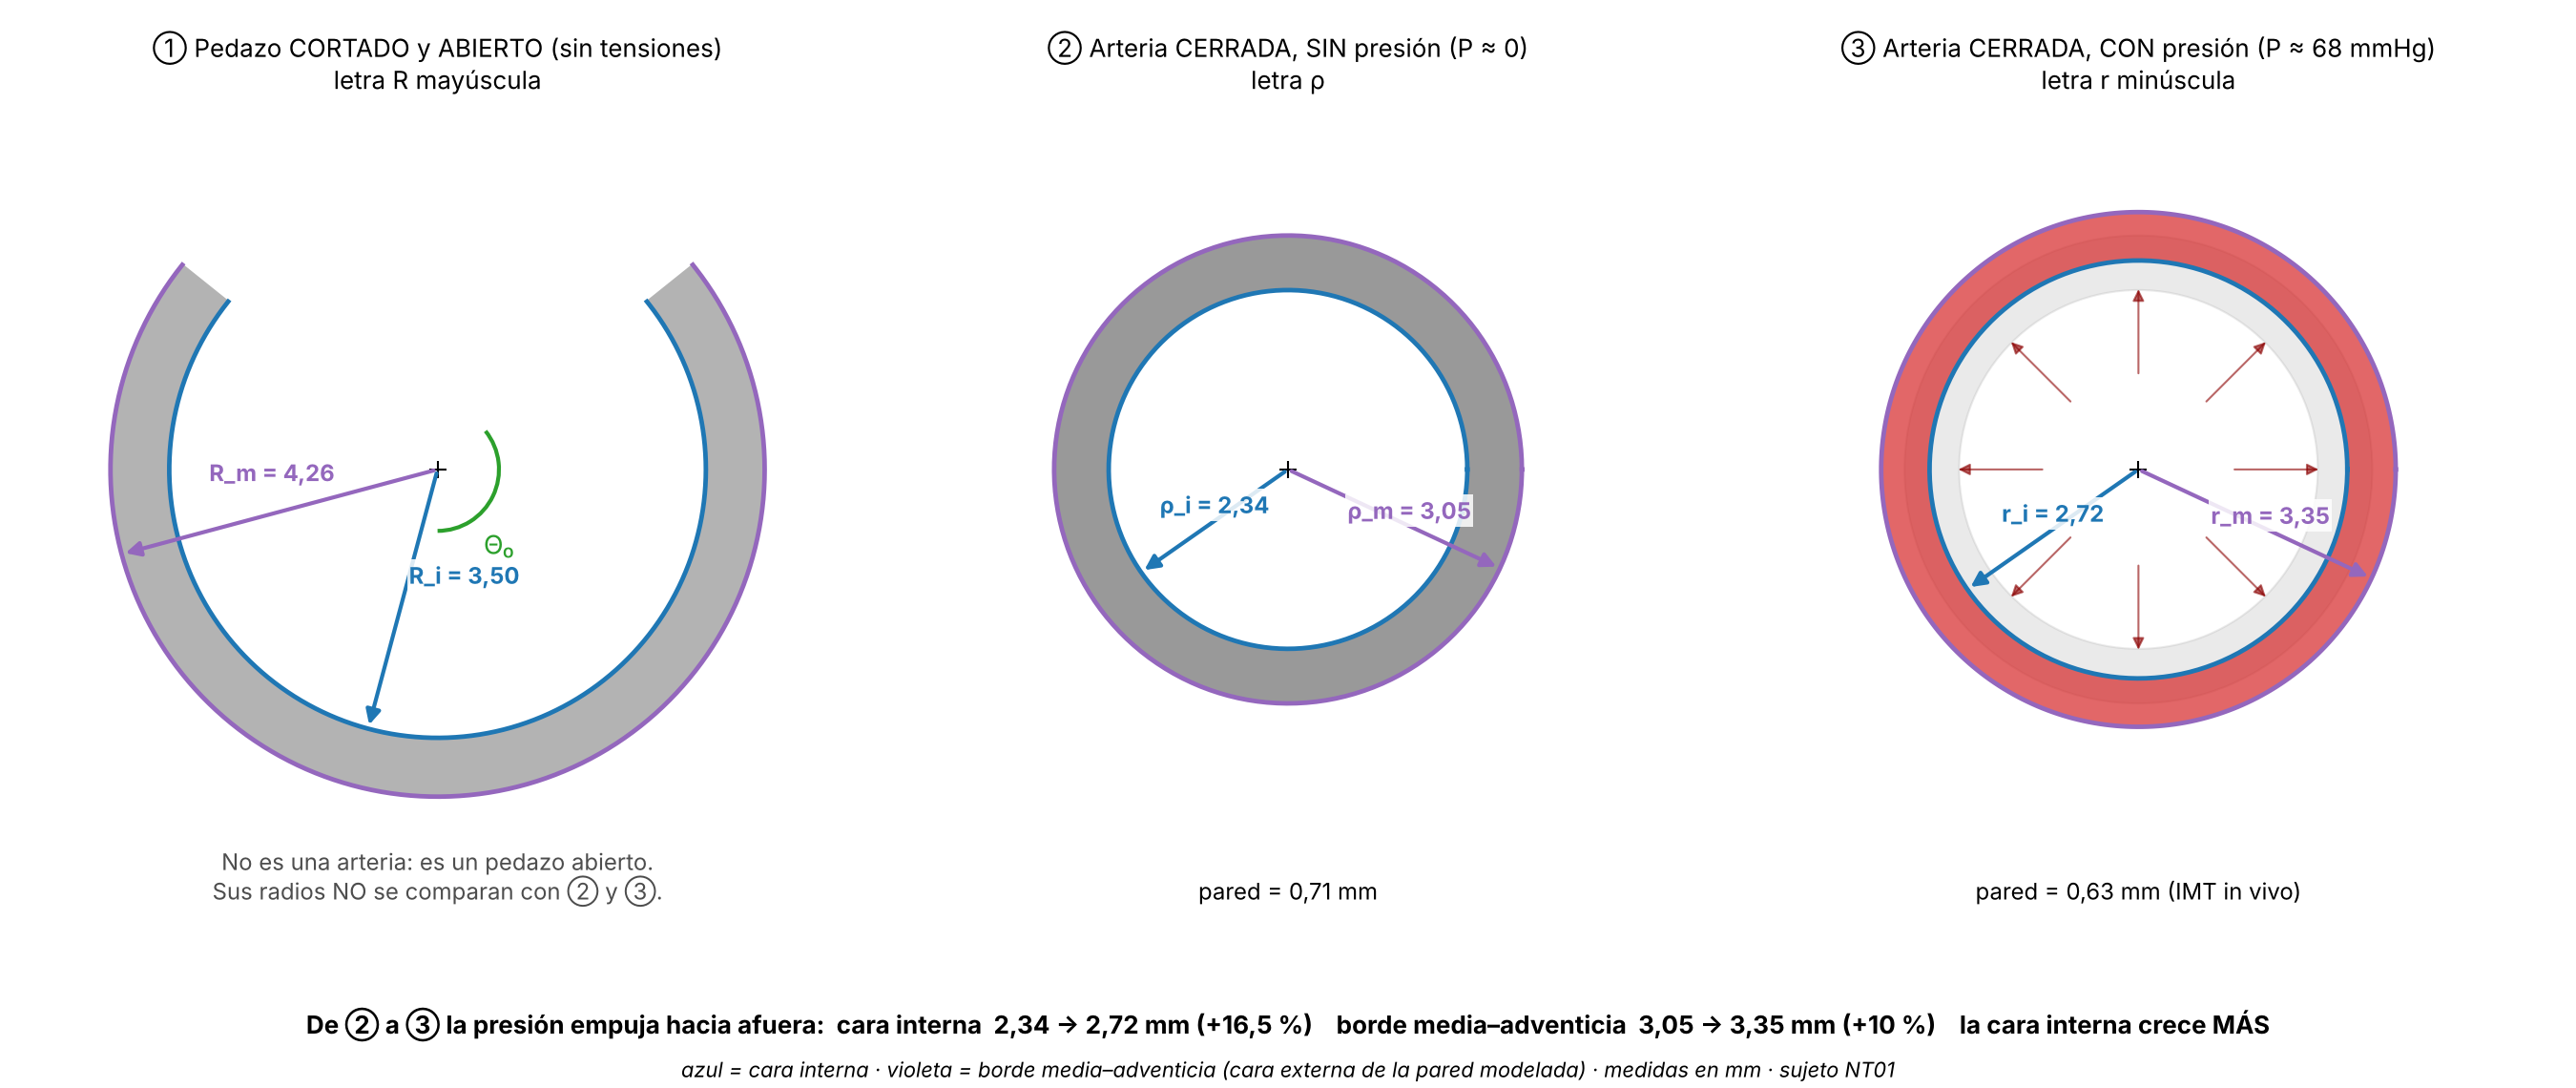
\includegraphics[width=\textwidth]{d10_tres_estados.png}
\caption{Subject NT01 in its three states: (1) stress-free open sector, (2) closed unpressurized artery, (3) pressurized artery. From (2) to (3) the inner surface grows by 16.5\,\% and the media--adventitia boundary by 10\,\%.}\label{fig:estados}\end{figure}

\paragraph{Pressure window.} What defines whether a state is physiological is the pressure, not the stretch: at $\lambda_\theta=1.16$ the stiffest subject bears about 400\,mmHg and a soft young subject about 70. Therefore, at this level, all subjects are evaluated in the same window, $P$ from 60 to 200\,mmHg (8.0 to 26.7\,kPa) at 141 values, which covers with a margin the measured mean pressures (64/116\,mmHg in NT and 73/127\,mmHg in HT~\cite{masson}). The target curve is the stretch of the media--adventitia boundary, $\lambda(P_k)$, proportional to the diameter (Fig.~\ref{fig:presion}): stiff subjects reach 200\,mmHg with $\lambda$ between 1.12 and 1.15, soft ones with $\lambda$ between 1.20 and 1.23.

\begin{figure}[H]\centering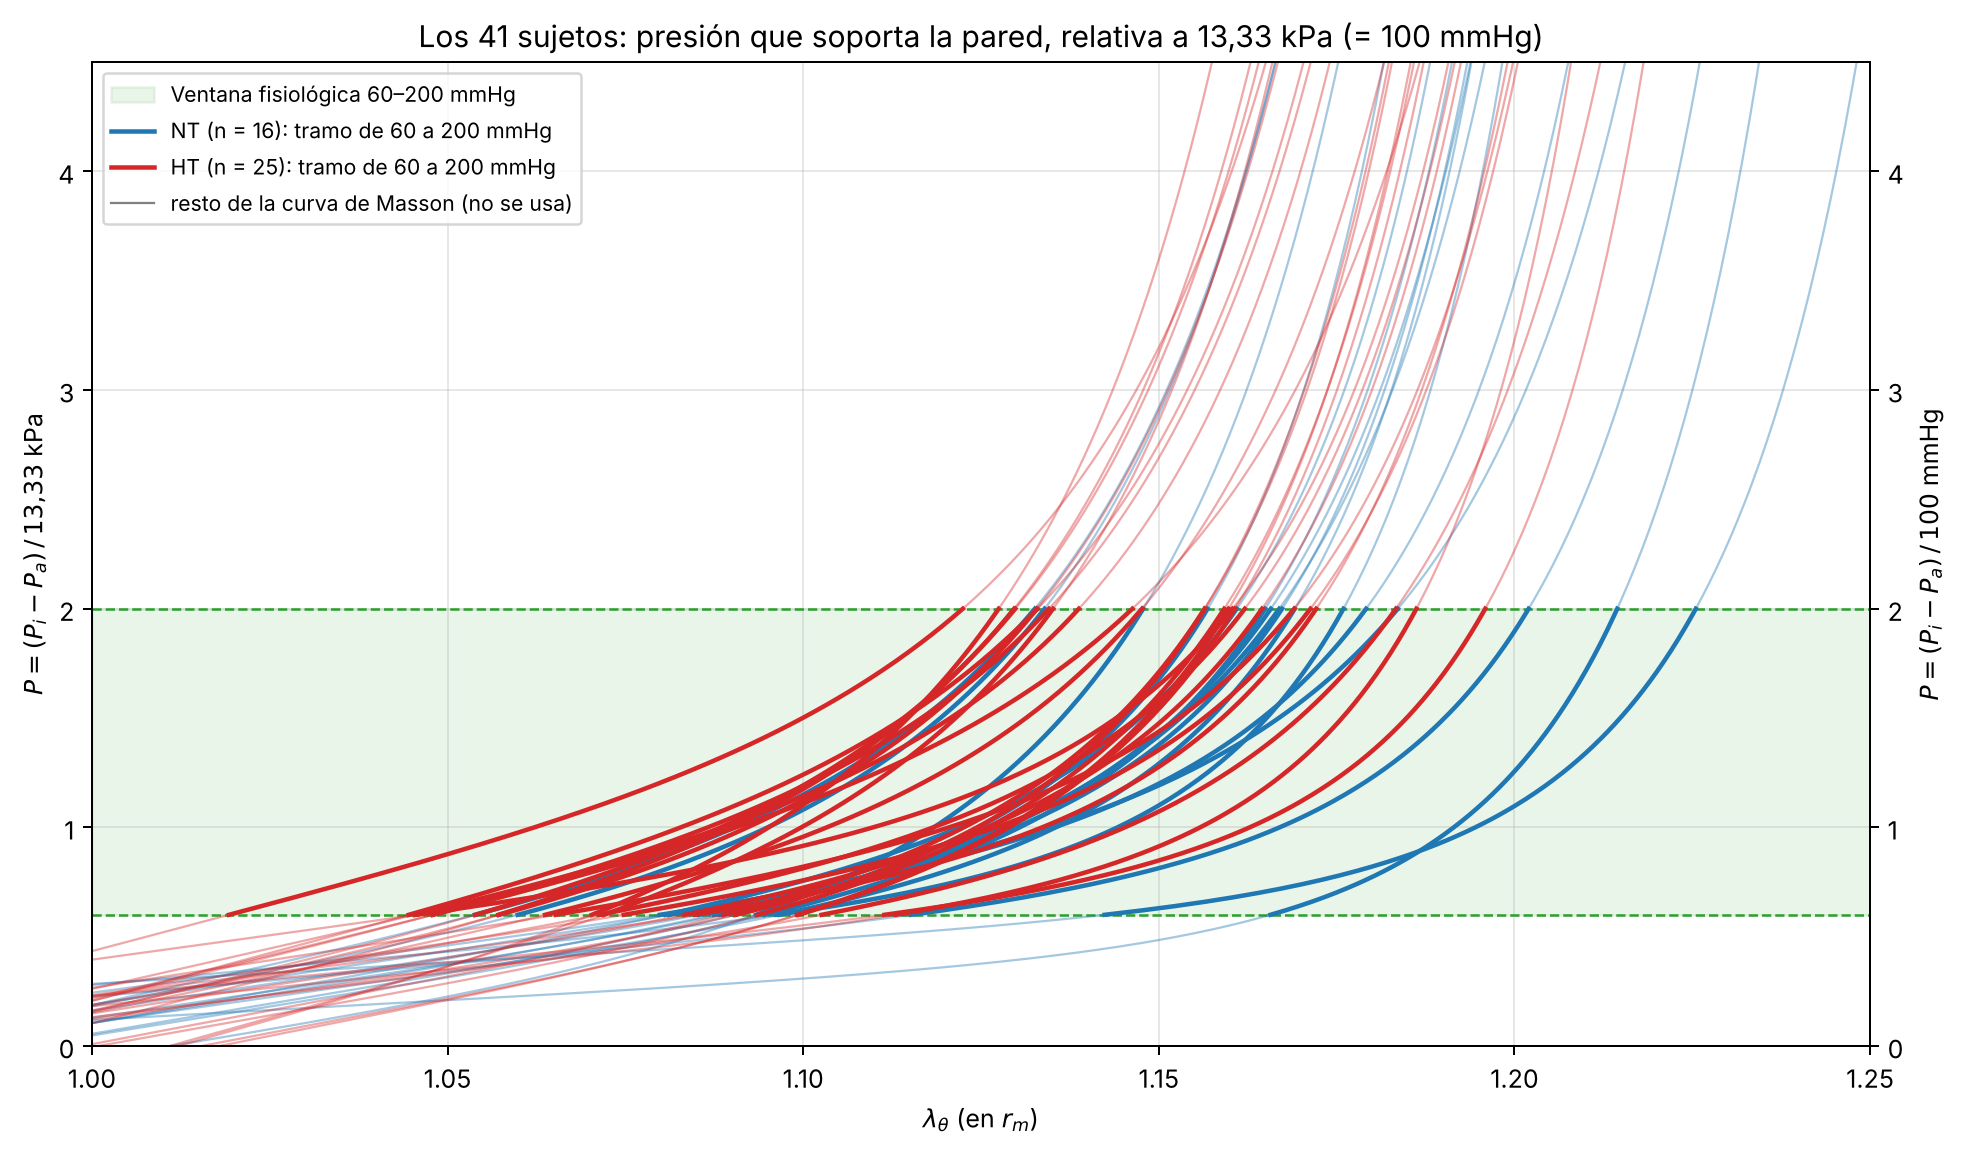
\includegraphics[width=0.85\textwidth]{f_sujetos_relativa.png}
\caption{The 41 subjects: pressure borne by the wall as a function of the stretch of the media--adventitia boundary, in relative form: $P=(P_i-P_a)/13.33$\,kPa on the left and $P=(P_i-P_a)/100$\,mmHg on the right. Since $13.33$\,kPa $=100$\,mmHg, both scales coincide; the 60 to 200\,mmHg window spans 0.6 to 2. Thick lines: the 60 to 200\,mmHg segment, which is the target curve.}\label{fig:presion}\end{figure}

\subsection{Thin wall and thick wall}
If the wall is thin compared with the radius, all its fibers stretch equally and the equilibrium of half a tube gives Laplace's law, $P=\sum_j\sigma_jh_j/r$~\cite{fung}: pressure is linear in the layer thicknesses and the design inherits the whole method of the first level. Urquiza~\cite{urquiza} (Eq.~3.13 of his thesis) writes the same thin-wall equilibrium with the \emph{instantaneous} radius and thickness, $(P_i-P_a)\,R=\sigma\,h$. Taking $R$ as the deformed mean radius, $\bar r=r_i+h/2$, and letting $u=1+h/r_i$,
\begin{equation}\label{eq:urquiza}
P=\frac{\sigma\,h}{r_i+h/2}=\sigma\,\frac{2\,(u-1)}{u+1}.
\end{equation}
For a homogeneous wall with uniform stress, \eqref{eq:equil} gives exactly $P=\sigma\ln u$, and $2(u-1)/(u+1)$ is the Padé [1/1] approximant of $\ln u$: for $h/r_i\le0.2$ the error is below 0.3\,\%, whereas Laplace's law with the inner radius, $P=\sigma\,(u-1)$, overestimates the pressure by up to 10\,\%. We call \emph{Urquiza's law} Eq.~\eqref{eq:urquiza} applied to the multilayer graft with a single stretch, that of the mean radius: $P=\sum_j\sigma_j(\bar\lambda)\,h_j/\bar r$, with $\bar\lambda=\bar r/\bar R$. It is still linear in the thicknesses. The carotid artery, however, has $h/r\approx0.2$. With an incompressible wall and no axial extension, the area between the inner surface and a fiber initially at radius $R$ is conserved,
\begin{equation}\label{eq:incomp}
r^2-r_i^2=R^2-R_i^2,\qquad\lambda(r)=\frac{r}{R},
\end{equation}
and inner fibers stretch more than outer ones (Fig.~\ref{fig:fibra}). The pressure is the exact sum of the contributions of each thin layer, each with its own stretch:
\begin{equation}\label{eq:pgruesa}
P=\sum_{j=1}^{N}\int_{\text{layer }j}\frac{\sigma_j\bigl(\lambda(r)\bigr)}{r}\,dr .
\end{equation}
If $h\ll r$, \eqref{eq:pgruesa} reduces to Laplace's law. With truncated lines, the difference in stretch decides whether a layer bears load or not: a material with knot 1.08 bears load at the inner surface of an inflated tube ($\lambda=1.10$) and not at the outer surface ($\lambda=1.07$). Moreover, the layers interact: if an inner layer grows, the outer ones are pushed to larger radii, stretch less and contribute less. In a thick wall, pressure is no longer linear in the thicknesses.

\begin{figure}[H]\centering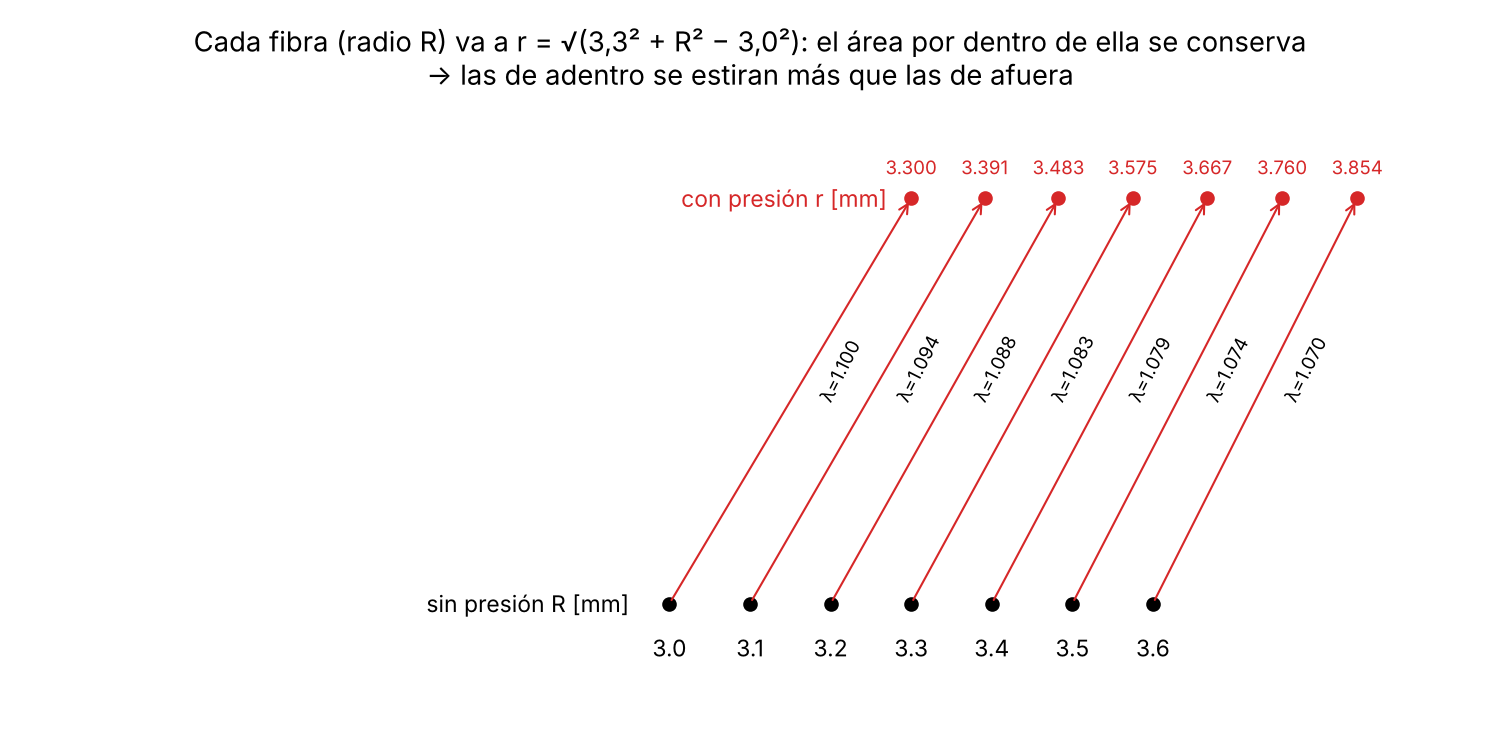
\includegraphics[width=0.78\textwidth]{d6_cada_fibra.png}
\caption{Tube from 3.0 to 3.6\,mm inflated to an inner radius of 3.3\,mm: each fiber conserves the area enclosed inside it; the inner surface stretches 10\,\% and the outer surface 7\,\%.}\label{fig:fibra}\end{figure}

\paragraph{The thin wall fails when manufactured.} Each subject was designed with three assumptions ---Laplace (thin wall, $P=\sigma h/r$ with the undeformed radius and thickness), Urquiza's law \eqref{eq:urquiza}, with the deformed mean radius, and thick wall (Eq.~\ref{eq:pgruesa}, each layer with its own stretch)--- and each design was evaluated in the real, thick-walled tube (Table~\ref{tab:laplace}, Fig.~\ref{fig:laplace}). In its own model, Laplace appears perfect ($e_{\max}\le1.7$\,\%); the error appears upon manufacturing and grows with wall thickness. Correcting the radius does not help, because the problem is not the radius but the fact that each layer stretches differently and engages at a different moment. With the pressure window and the adopted basis, the linear thin-wall design does not meet the target in any subject either (median 27.3\,\% with 6 materials and 29.9\,\% with 5). \textbf{The tube-level design must be carried out with the thick-walled model.}

\begin{table}[H]\centering\small
\caption{Comparison of assumptions on pressure curves for $\lambda$ from 1.02 to 1.16, with a set of knots fitted to those pressure curves (different from that of Table~\ref{tab:bases}). Each row is the assumption used to \emph{design}; all designs are \emph{evaluated} in the thick-walled tube, which is what is manufactured. In each cell, for the 41 subjects: how many meet $e_{\max}\le3$\,\%, the median $e_{\max}$ and the worst $e_{\max}$, with 5 or 6 materials.}\label{tab:laplace}
\begin{tabular}{lcc}\toprule
Design assumption & 5 materials & 6 materials\\\midrule
Laplace & 0/41 · 13.6\,\% · 22.7\,\% & 0/41 · 14.8\,\% · 32.5\,\%\\
Urquiza (deformed mean radius) & 0/41 · 13.7\,\% · 24.5\,\% & 0/41 · 15.4\,\% · 34.4\,\%\\
Thick wall & 41/41 · 0.96\,\% · 2.97\,\% & 41/41 · 0.72\,\% · 2.10\,\%\\\bottomrule
\end{tabular}
\end{table}
\begin{figure}[H]\centering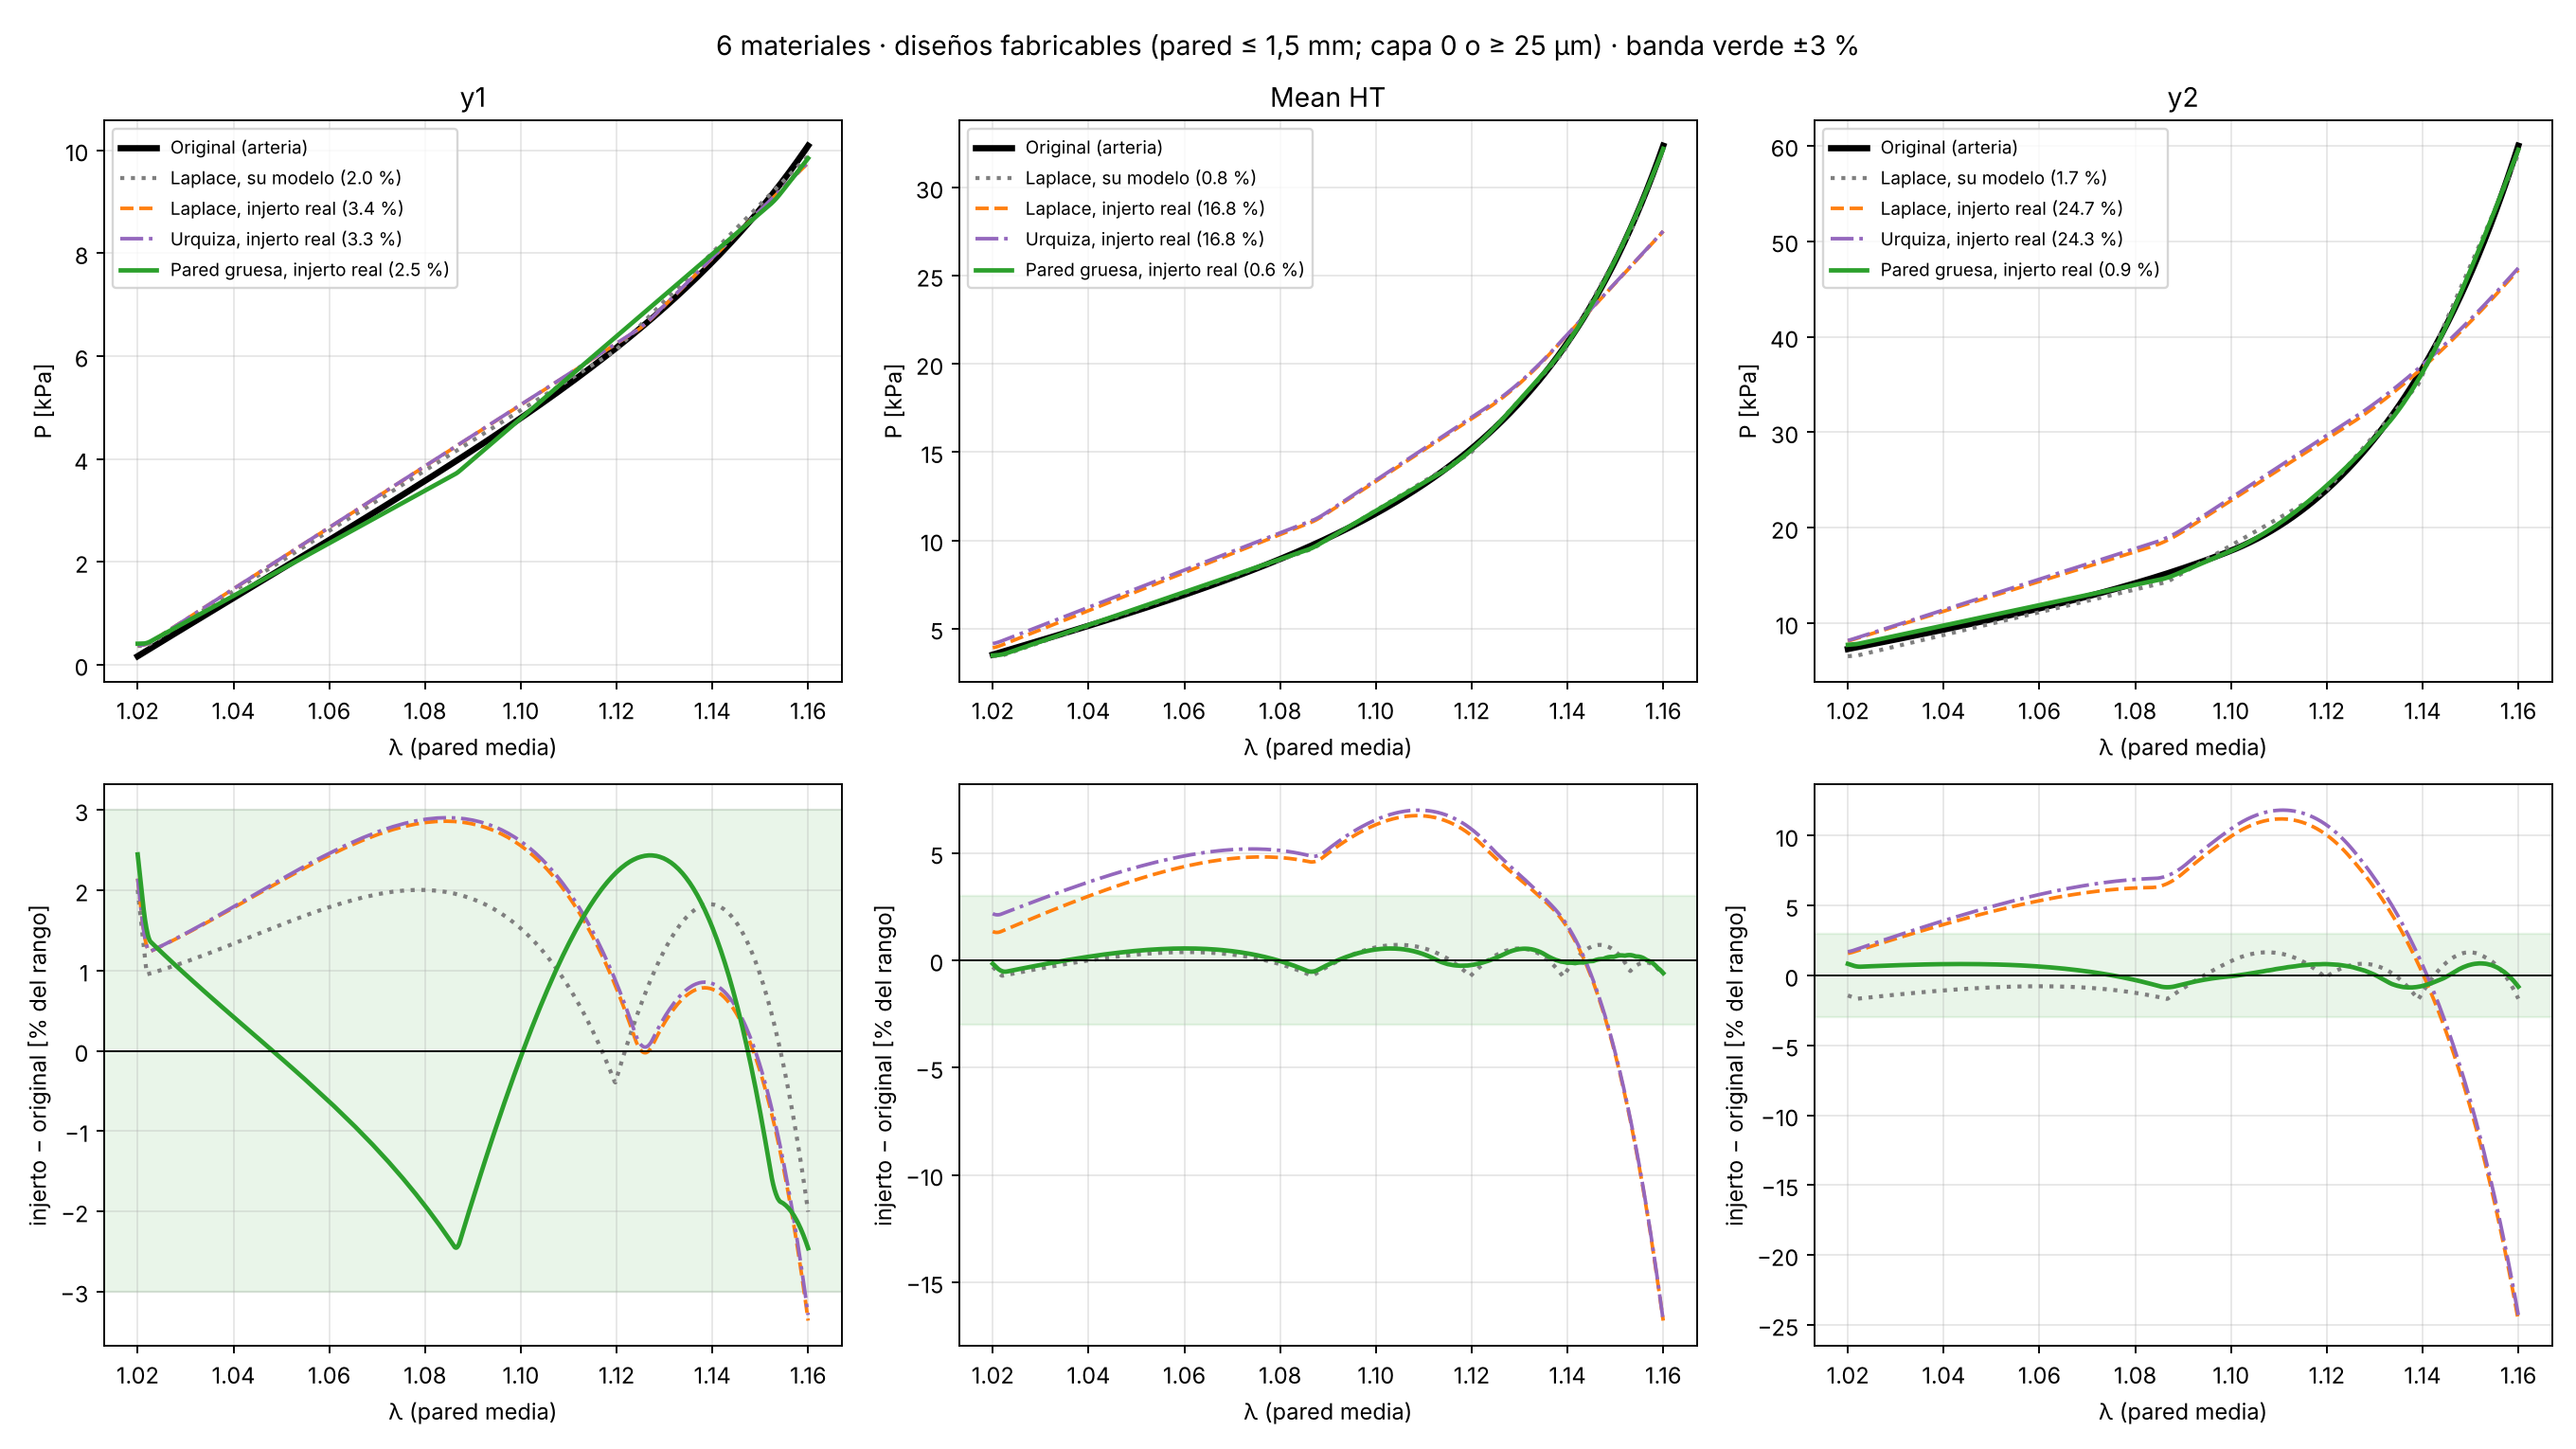
\includegraphics[width=0.82\textwidth]{f34_3c_6.png}
\caption{Conditions of Table~\ref{tab:laplace}, 6 materials, from left to right: softest curve ($y_1$), hypertensive mean and stiffest curve ($y_2$). Top of each pair: curves; bottom: graft $-$ artery in \% of the range (band $\pm3$\,\%). The Laplace design evaluated in its own model (gray, dotted) appears perfect; once manufactured (orange, dashed) it departs by up to 25\,\%.}\label{fig:laplace}\end{figure}
\begin{table}[H]\centering\small
\caption{Designs of Fig.~\ref{fig:laplace} (pressure curves for $\lambda$ from 1.02 to 1.16, 6 materials; knots 0.8271, 1.0219, 1.0867, 1.1197, 1.1391, 1.1531 and moduli 0.18, 1.33, 4.86, 2.72, 12.94, 6.35\,MPa): thickness of the layer of each material $h_j$ [µm] (layer 1 next to the blood; 0: not used), total wall [µm] and errors against the pressure curve of the artery, $E_{\mathrm{rms}}$ and $e_{\max}$ [\% of the range]. ``Laplace, own model'' and ``Laplace, real graft'' are the same design evaluated with two models.}\label{tab:laplace3}
\resizebox{\textwidth}{!}{%
\begin{tabular}{llccccccccc}\toprule
Curve & Design and evaluation & $h_1$ & $h_2$ & $h_3$ & $h_4$ & $h_5$ & $h_6$ & wall & $E_{\mathrm{rms}}$ & $e_{\max}$\\\midrule
$y_1$ & Laplace, own model & 25 & 153 & 0 & 56 & 0 & 0 & 233 & 1.47 & 2.01\\
 & Laplace, real graft & 25 & 153 & 0 & 56 & 0 & 0 & 233 & 1.98 & 3.36\\
 & Urquiza, real graft & 25 & 153 & 0 & 56 & 0 & 0 & 233 & 2.01 & 3.29\\
 & Thick wall, real graft & 25 & 130 & 25 & 0 & 0 & 29 & 210 & 1.47 & 2.46\\
\addlinespace
HT mean & Laplace, own model & 235 & 203 & 59 & 205 & 67 & 136 & 905 & 0.41 & 0.76\\
 & Laplace, real graft & 235 & 203 & 59 & 205 & 67 & 136 & 905 & 5.14 & 16.79\\
 & Urquiza, real graft & 250 & 196 & 62 & 204 & 66 & 132 & 909 & 5.40 & 16.79\\
 & Thick wall, real graft & 129 & 158 & 48 & 218 & 0 & 467 & 1020 & 0.34 & 0.60\\
\addlinespace
$y_2$ & Laplace, own model & 449 & 229 & 139 & 461 & 193 & 30 & 1500 & 1.08 & 1.73\\
 & Laplace, real graft & 449 & 229 & 139 & 461 & 193 & 30 & 1500 & 7.95 & 24.69\\
 & Urquiza, real graft & 453 & 241 & 141 & 454 & 187 & 25 & 1500 & 8.24 & 24.30\\
 & Thick wall, real graft & 203 & 122 & 67 & 626 & 206 & 277 & 1500 & 0.61 & 0.87\\
\bottomrule
\end{tabular}}
\end{table}

\subsection{The thick-walled graft}
The graft is a closed, incompressible tube in plane strain, with one layer per material stacked from inside to outside in order of increasing knot (the reverse order doubles or triples the error), centered at $R_{\mathrm{ref}}=3.421$\,mm (median of $\Theta_0R_m/\pi$ over the 41 subjects). The materials are those of the first level: the same knots and lines $\sigma_j=E_j\max(0,\lambda-\kappa_j)$, with moduli $E_j$ calibrated once so that the training subject that needs the most of each material uses 0.2\,mm of it (6 materials: from 452 to 4966\,kPa). The design is
\begin{equation}\label{eq:theta}
\theta=(h_1,\dots,h_N,\ \delta),\qquad 0\le h_j\le3\ \text{mm},\quad|\delta|\le0.25.
\end{equation}
Here $h_j$ is the thickness of the layer of material $j$ and $\delta$ is the \emph{common prestretch}: a shift of all the knots together, in units of stretch (dimensionless). Layer $j$ starts working when the mid-wall reaches $k_j+\delta$ instead of $k_j$:
\begin{itemize}
\item $\delta<0$ advances the engagement of all layers (they are mounted tighter: they bear load earlier);
\item $\delta=0$ keeps the knots of the first-level basis;
\item $\delta>0$ delays it (they are mounted looser: they bear load later).
\end{itemize}
\textbf{Meaning of $|\delta|\le0.25$.} $|\delta|$ is the absolute value of $\delta$, so the condition is equivalent to $-0.25\le\delta\le0.25$: the knots can be shifted by at most 0.25 to the left or to the right. For example, with $\delta=-0.25$ the knot 1.08 moves to 0.83, and with $\delta=+0.25$, to 1.33. It is a bound of the search, not a material property: it was chosen wider than the whole stretch interval spanned by a subject (from 1.02 to 1.23, i.e.\ 0.21), so that no subject is excluded by the bound. It is not active: in the 82 designs (41 subjects, 5 and 6 materials) $\delta$ remained between $-0.04$ and $+0.09$. Appendix~\ref{sec:ejemplo} shows, with an example that can be checked by hand, what $\delta$ does in a two-layer tube.
\begin{itemize}
\item \textbf{Thicknesses} $h_j$, manufactured with $n_j$ integer laminae of thickness $e$.
\item \textbf{Engagement and prestretch.} Each layer engages when the mid-wall reaches $k_j+\delta$; its local engagement stretch $\kappa_j$ is the stretch of the layer center at that moment, from \eqref{eq:incomp}. In manufacturing, $\kappa_j$ is the crimp of the fibers of that layer. The common prestretch $\delta$ shifts all the knots together: each subject occupies its own stretch interval (from 1.02 to 1.23), and without $\delta$ it would see only one or two knots, with a typical error of 11\,\%.
\end{itemize}
The pressure \eqref{eq:pgruesa} is integrated in each layer with 8-node Gauss--Legendre quadrature~\cite{davis} at 651 values of $\lambda$ between 0.80 and 1.45, and inverted by linear interpolation to obtain $\lambda_{\mathrm{gr}}(P_k;\theta)$. The map $\theta\mapsto\lambda_{\mathrm{gr}}$ is nonlinear: the thicknesses set the integration limits and the engagements, and $\delta$ enters inside the $\max(0,\cdot)$. With integer laminae, finding the $n_j$ is a \textbf{mixed-integer nonlinear} problem. The metric is \eqref{eq:emax} on $\lambda(P_k)$.

\subsection{Design methods}
\begin{table}[H]\centering\small
\caption{Computational blocks at the tube level. ``Linear'' refers to the dependence of the model on the unknowns.}\label{tab:bloques}
\resizebox{\textwidth}{!}{%
\begin{tabular}{>{\raggedright\arraybackslash}p{3.0cm}>{\raggedright\arraybackslash}p{2.2cm}>{\raggedright\arraybackslash}p{1.6cm}>{\raggedright\arraybackslash}p{5.0cm}>{\raggedright\arraybackslash}p{4.1cm}}\toprule
Block & Variables & Linear? & Algorithm & Implementation\\\midrule
A1 Linear LS (thin wall) & real & yes, with fixed $\delta$ & least squares by SVD; $\delta$ by grid and Brent & \texttt{numpy.linalg.lstsq}~\cite{numpy}; \texttt{minimize\_scalar}~\cite{brent,scipy}\\
A2 Nonlinear LS (thick wall) & real & no & trust region reflective with bounds (TRF) & \texttt{scipy.optimize.least\_squares}~\cite{branch,scipy}\\
A3 Integer minimax (thick wall) & integer laminae, real $\delta$ & no & floor/ceiling enumeration, $\delta$ by bounded Brent, local search & own code; \texttt{minimize\_scalar}~\cite{brent}\\
A4 Neural network & real & --- (one evaluation) & multilayer perceptron; amortized optimization & TensorFlow/Keras~\cite{tf}\\\bottomrule
\end{tabular}}
\end{table}

\paragraph{A1 · Linear thin-wall least squares.} With Laplace's law and fixed $\delta$, pressure is linear in $c_j=E_jh_j/R_{\mathrm{ref}}$: $P_k\approx\sum_jc_j\max(0,y_k-k_j-\delta)$. For each $\delta$ on a grid of 101 values the problem is solved by least squares; the pressure residual is converted to $\lambda$ with the local slope of the curve; the best $\delta$ is refined by Brent's method~\cite{brent} and $h_j=c_jR_{\mathrm{ref}}/E_j$, clipped to $[0,3]$\,mm. It is the first-level method transferred to the tube.

\paragraph{A2 · Nonlinear thick-wall least squares.} It minimizes $\sum_k\bigl((\lambda_{\mathrm{gr}}(P_k;\theta)-y_k)/\Delta\bigr)^2$ subject to the bounds \eqref{eq:theta}, by the Trust Region Reflective (TRF) method~\cite{branch}. At each iteration it computes the Jacobian of the residuals by finite differences, approximates the problem by its Gauss--Newton quadratic model and takes the step that minimizes it within a \emph{trust region}, a neighborhood where the model is reliable; it enlarges the region if the step succeeded and shrinks it otherwise, and reflects inward the steps that cross a bound. Tolerances $10^{-10}$, at most 300 evaluations. It finds a \emph{local} minimum: the result depends on the starting point.

\paragraph{A3 · Integer minimax.} It is the first-level minimax extended to the nonlinear case, where no linear program can solve it exactly. Starting from a real-valued design $\theta^\star$ and a reference curve $\tilde y$: (1) $n_j\in\{\lfloor h_j^\star/e\rfloor,\lceil h_j^\star/e\rceil\}$; the $2^N$ combinations are evaluated by $e_{\max}$ against $\tilde y$; (2) for the 8 best ones, $\delta$ is readjusted within $\pm0.03$ by bounded Brent; (3) local search~\cite{aarts}: neighbors that add or remove one lamina of a material or move one lamina from one material to another, accepting the best one if it lowers the worst error, up to 20 times. It is a heuristic: it does not guarantee the global integer optimum. Unlike the first level, here a real-valued solution is indeed the starting point: this is the usual strategy for nonlinear integer problems, solving the continuous problem and searching for integers in its neighborhood, and it is reasonable because with 0.025\,mm laminae a design has about 46 laminae and one lamina shifts the curve only slightly. The distance of this heuristic from the optimum is measured below (\emph{Distance to the integer optimum}).

\paragraph{A4 · Neural network.} The same architecture as in the first level, $141\to256\to128\to64\to N{+}1$: it receives the standardized curve $\lambda(P_k)$ and returns $\theta$. Data: 6000 grafts with randomly drawn designs, whose label is exactly their design, and 9000 synthetic arteries of Masson's law plus the 31 training subjects, whose label is the A2 fit; new noise of 0 to 1\,\% of the range of $\lambda$ at each epoch. Split 11\,220 / 1530 / 2250; 425 epochs (6 materials) and 629 (5). It is used as \emph{amortized optimization}~\cite{amos}: a model learned on many solved cases proposes the solution of a new one, and a classical optimizer finishes it. Learning curves and metrics are given in Appendix~\ref{sec:entrenamiento}.

\paragraph{The procedure.} The blocks are chained in three steps (Fig.~\ref{fig:proc}): (1) initialization, A1 (path A) or the network A4 (path B); (2) A2, which fits the design to the curve; (3) A3, which chooses the laminae against the \emph{fitted curve} of step 2. This is the first-level conclusion about noise: step 2 smooths, because the curve of a graft cannot have the jumps of the noise, and step 3 does not chase it.

\begin{figure}[H]\centering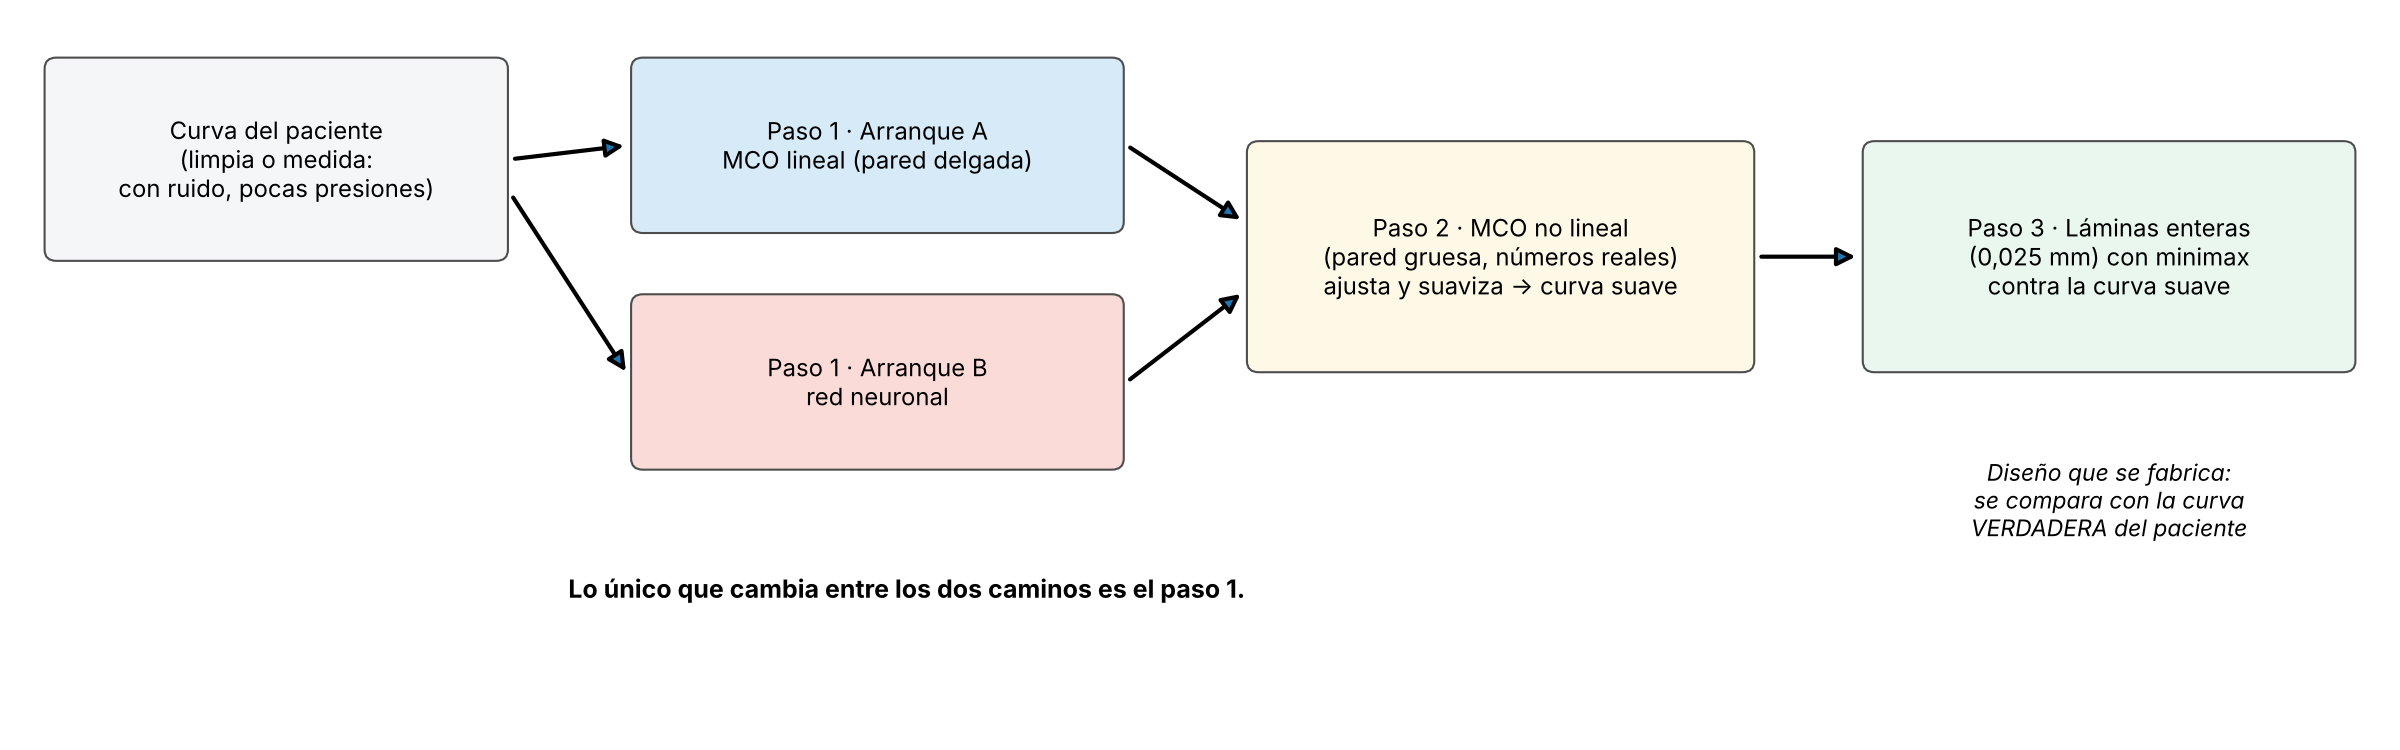
\includegraphics[width=\textwidth]{f_procedimiento.png}
\caption{The tube-level design procedure. The two paths differ only in step 1.}\label{fig:proc}\end{figure}

\paragraph{Measured curves.} In practice the patient's curve is measured, with noise and at few pressures. We simulate: (a) proportional Gaussian noise of 0.3\,\% in $\lambda$ (echotracking resolves about 20\,µm in 7\,mm); (b) measurement at 10 pressures with monotone cubic interpolation (PCHIP)~\cite{pchip} to the 141; (c) both, with 0.2\,\% noise. Each path receives the measured curve and its integer design is compared with the true curve; one realization per subject and case. Since $\lambda\approx1.1$ and its range is about 0.07, a noise of 0.3\,\% of $\lambda$ corresponds to about 5\,\% of the range: larger than the target.

\subsection{Results}
\paragraph{Real-valued design.} From the linear initialization, A2 brings 40 of the 41 subjects within the target (6 materials: median 0.84\,\%, worst 3.43\,\%; 5 materials: 40/41, worst 3.14\,\%), with walls from 0.75 to 1.89\,mm and $\delta$ from $-0.04$ to $+0.09$. Starting from the network it reaches 41 of 41 with 6 materials (worst 1.79\,\%), with half the model evaluations (16 versus 35 per subject). On its own, the network falls short: median 3.43\,\% and worst 89.6\,\%. In the 10 test subjects the hybrid gives a median of 0.93\,\% and a worst case of 1.79\,\%.

\paragraph{Lamina thickness.} With laminae of 0.1, 0.05 and 0.025\,mm, 38, 40 and 41 of the 41 subjects met the target (6 materials; worst 5.44, 3.69 and 1.64\,\%; about 10, 23 and 46 laminae). We adopted $e=0.025$\,mm.

\paragraph{The complete procedure.} With clean curves both initializations tie (Table~\ref{tab:f2}, Fig.~\ref{fig:dis47}). The difference lies in the worst case with measured curves: with 10 pressures, the linear initialization falls into a local minimum in two subjects (NT03 and HT04, 468.7\,\%), which the network initialization avoids; with 0.3\,\% noise, the network increases the number of subjects within the target (31 versus 23 with 6 materials; 32 versus 25 with 5). With 10 pressures and noise, none exceeds 8 of 41: that noise is already comparable to the target. The time is 0.2 to 0.5\,s per subject with either initialization.

\paragraph{Distance to the integer optimum.} To measure how much the A3 heuristic loses, for the 41 subjects (clean curves, linear LS initialization) we enumerated \emph{all} combinations of laminae within $\pm2$ of those of the real-valued design of step 2 (up to $5^6=15\,625$ combinations), each with $\delta$ on a grid of 13 values and refined by Brent's method for the best 200, with the same objective as A3 (worst point against the fitted curve). The exhaustive search yields the same design as A3 in 24 of the 41 subjects (6 materials) and in 34 (5 materials); the worst point decreases in 20 subjects (6 materials), on average by 0.15 and at most by 0.44 points, and in 10 subjects with 5 materials (0.14 and 0.43; sometimes with the same laminae and a different $\delta$). Against the true curve, the median goes from 1.13 to 1.03\,\% (6 materials) and from 1.69 to 1.62\,\% (5), and neither the worst case (3.26 and 3.21\,\%) nor the number of subjects meeting the target (40 of 41 in both cases) changes. The heuristic therefore stays within a few tenths of a point of the optimum in that neighborhood, in 0.5\,s instead of the 2\,min per subject of the exhaustive search (6 materials).

\begin{table}[H]\centering\small
\caption{Complete procedure with 0.025\,mm laminae: worst error against the true curve [\%], 41 subjects.}\label{tab:f2}
\resizebox{\textwidth}{!}{%
\begin{tabular}{llcccccc}\toprule
 & & \multicolumn{3}{c}{6 materials} & \multicolumn{3}{c}{5 materials}\\\cmidrule(lr){3-5}\cmidrule(lr){6-8}
Curve & Initialization & median & worst & meet & median & worst & meet\\\midrule
clean & linear LS & 1.13 & 3.26 & 40/41 & 1.69 & 3.21 & 40/41\\
 & network & 1.14 & 2.19 & 41/41 & 1.68 & 3.19 & 40/41\\\addlinespace
10 pressures & linear LS & 1.26 & 468.7 & 38/41 & 1.62 & 3.13 & 40/41\\
 & network & 1.19 & 2.27 & 41/41 & 1.61 & 2.70 & 41/41\\\addlinespace
noise 0.3\,\% & linear LS & 2.67 & 11.87 & 23/41 & 2.66 & 7.52 & 25/41\\
 & network & 2.19 & 6.59 & 31/41 & 2.32 & 9.24 & 32/41\\\addlinespace
10 pres. + noise 0.2\,\% & linear LS & 4.36 & 8.07 & 8/41 & 4.62 & 8.77 & 6/41\\
 & network & 3.78 & 8.54 & 8/41 & 4.75 & 10.35 & 6/41\\\bottomrule
\end{tabular}}
\end{table}

\begin{figure}[H]\centering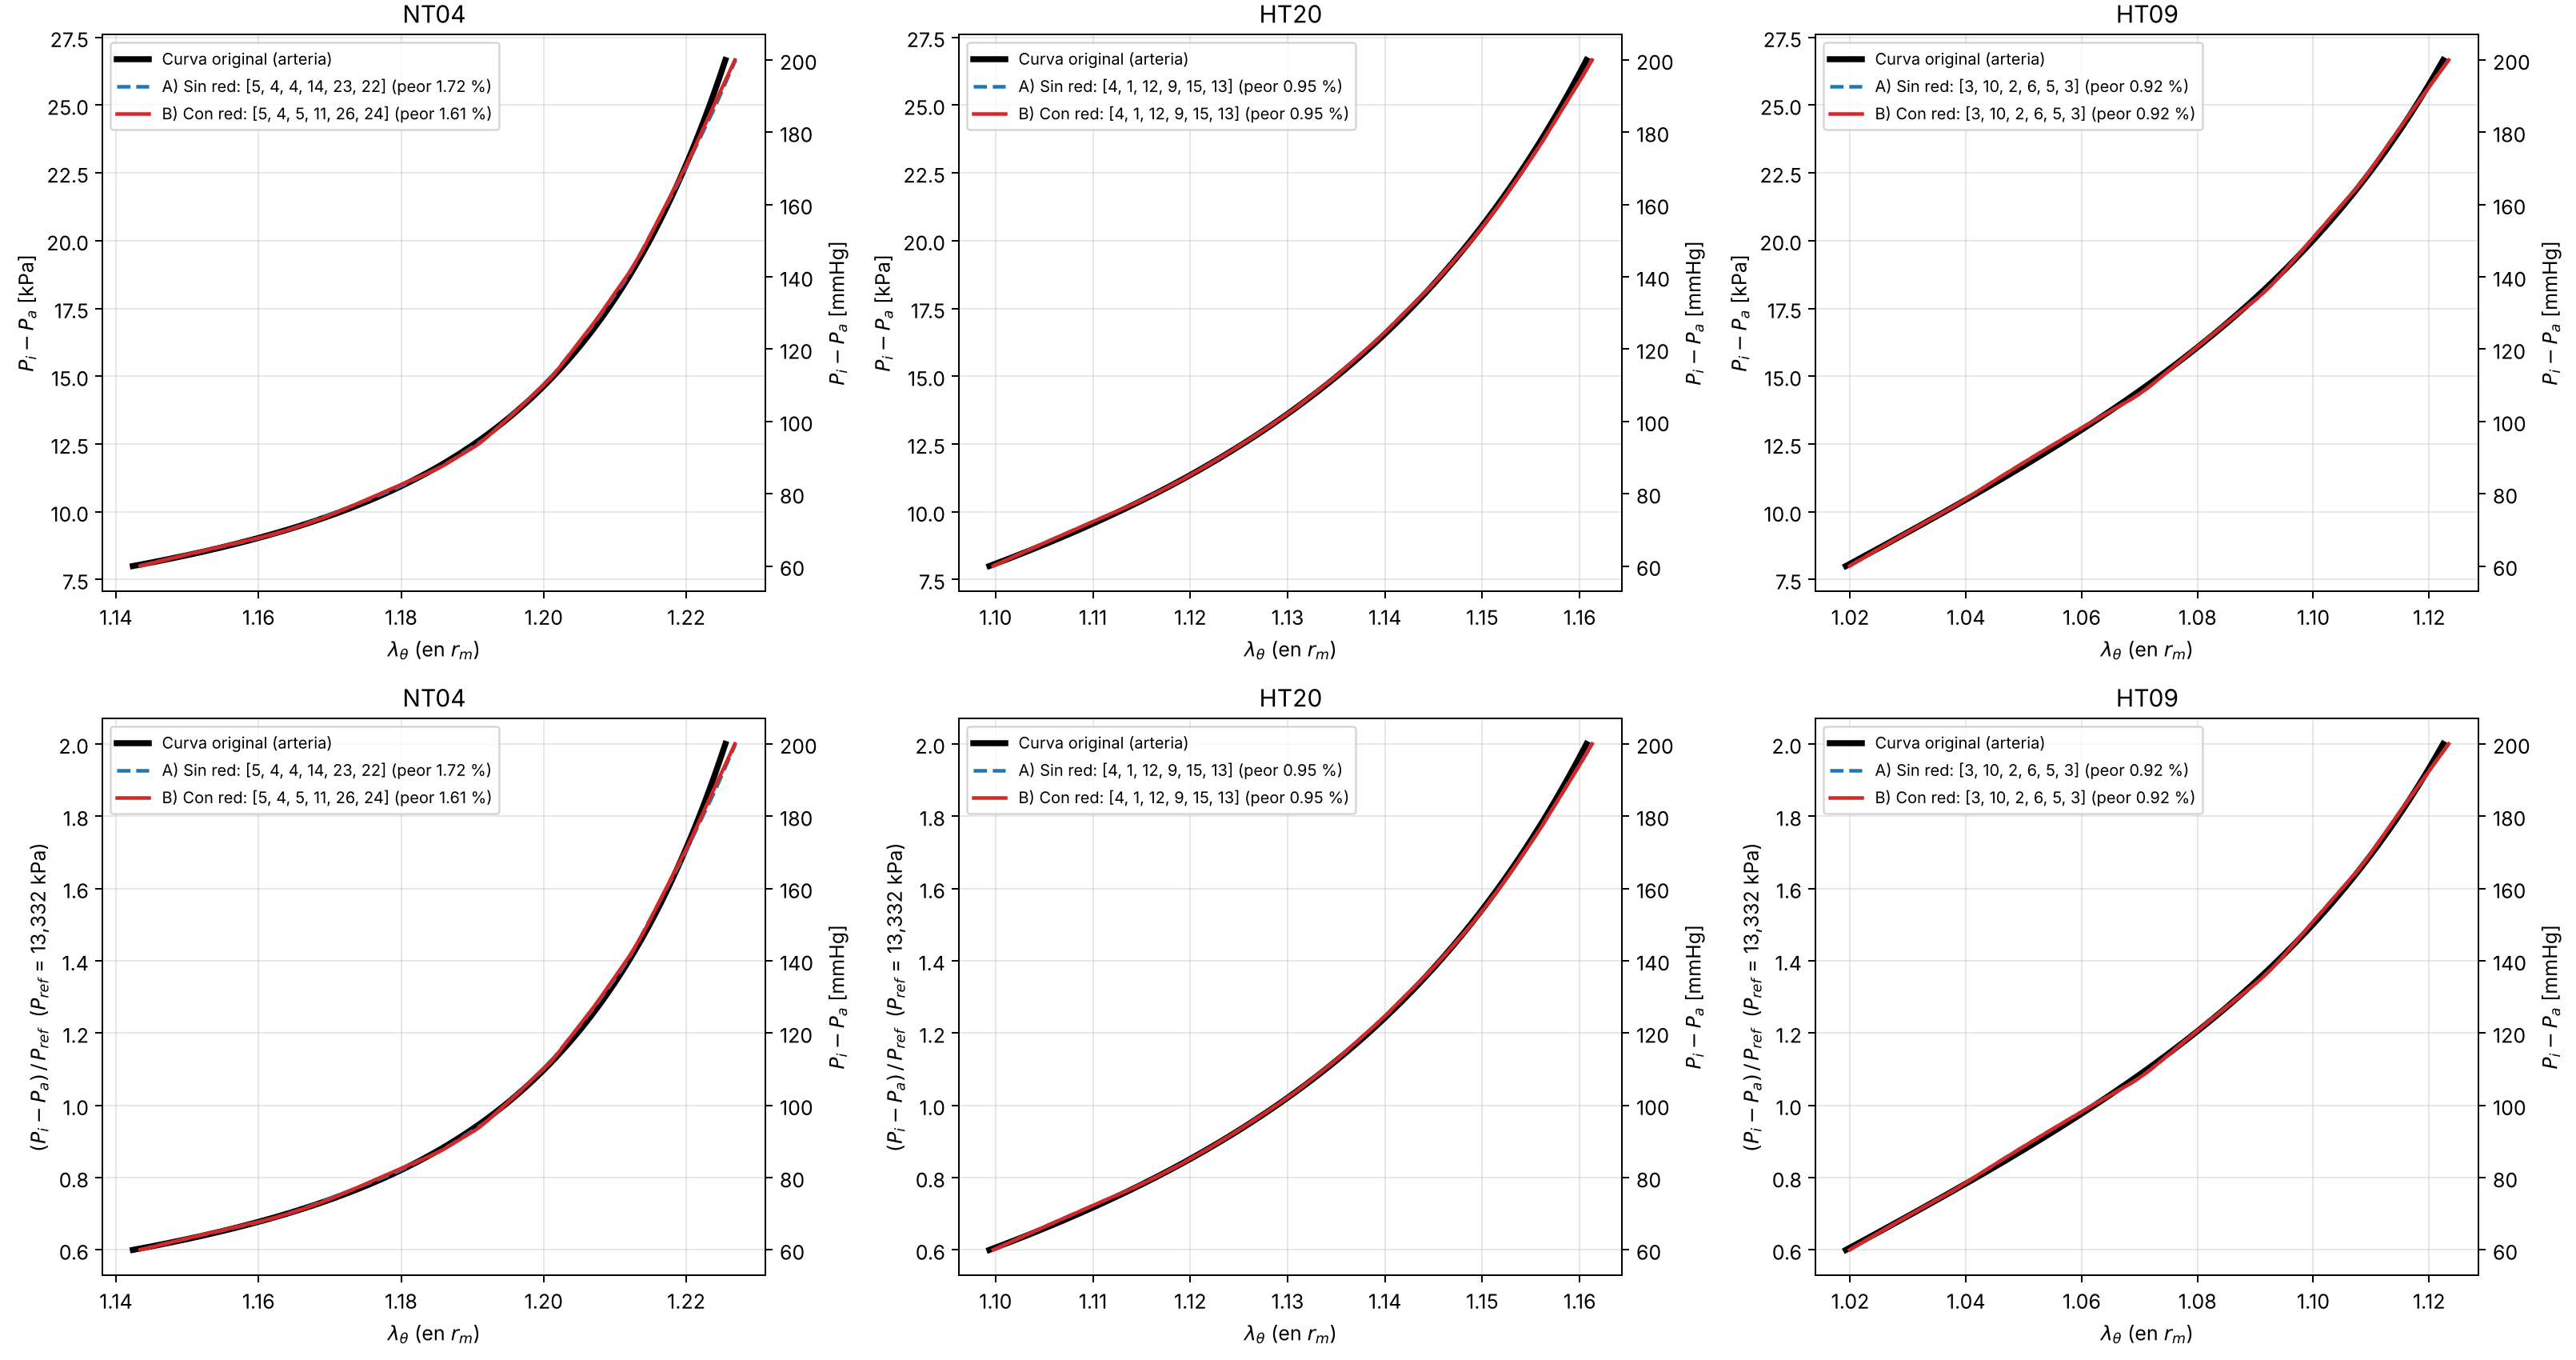
\includegraphics[width=\textwidth]{disenos_6_sin_titulo.png}
\caption{6 materials, clean curves: the softest subject, an intermediate one and the stiffest one. Black: artery; blue: path A (linear LS initialization); red: path B (network initialization). Ordinate: pressure borne by the wall, in kPa at the top and relative to 13.332\,kPa at the bottom; mmHg on the right. In brackets, laminae of each material.}\label{fig:dis47}\end{figure}
\begin{table}[H]\centering\small
\caption{Integer designs of Fig.~\ref{fig:dis47} (6 materials, 0.025\,mm laminae, clean curves): number of laminae of each material $n_j$ (material 1 next to the blood), total laminae, wall [mm], prestretch $\delta$ and errors against the $\lambda(P)$ curve of the artery, $E_{\mathrm{rms}}$ and $e_{\max}$ [\% of the range]. Path A: linear LS initialization; path B: network initialization.}\label{tab:dis47}
\resizebox{\textwidth}{!}{%
\begin{tabular}{llccccccccccc}\toprule
Subject & Path & $n_1$ & $n_2$ & $n_3$ & $n_4$ & $n_5$ & $n_6$ & laminae & wall & $\delta$ & $E_{\mathrm{rms}}$ & $e_{\max}$\\\midrule
NT04 (softest) & A & 5 & 4 & 4 & 14 & 23 & 22 & 72 & 1.800 & $+0.0861$ & 0.59 & 1.72\\
 & B & 5 & 4 & 5 & 11 & 26 & 24 & 75 & 1.875 & $+0.0890$ & 0.58 & 1.61\\
\addlinespace
HT20 (intermediate) & A & 4 & 1 & 12 & 9 & 15 & 13 & 54 & 1.350 & $+0.0103$ & 0.37 & 0.95\\
 & B & 4 & 1 & 12 & 9 & 15 & 13 & 54 & 1.350 & $+0.0103$ & 0.37 & 0.95\\
\addlinespace
HT09 (stiffest) & A & 3 & 10 & 2 & 6 & 5 & 3 & 29 & 0.725 & $-0.0394$ & 0.42 & 0.92\\
 & B & 3 & 10 & 2 & 6 & 5 & 3 & 29 & 0.725 & $-0.0394$ & 0.42 & 0.92\\
\bottomrule
\end{tabular}}
\end{table}

\begin{figure}[H]\centering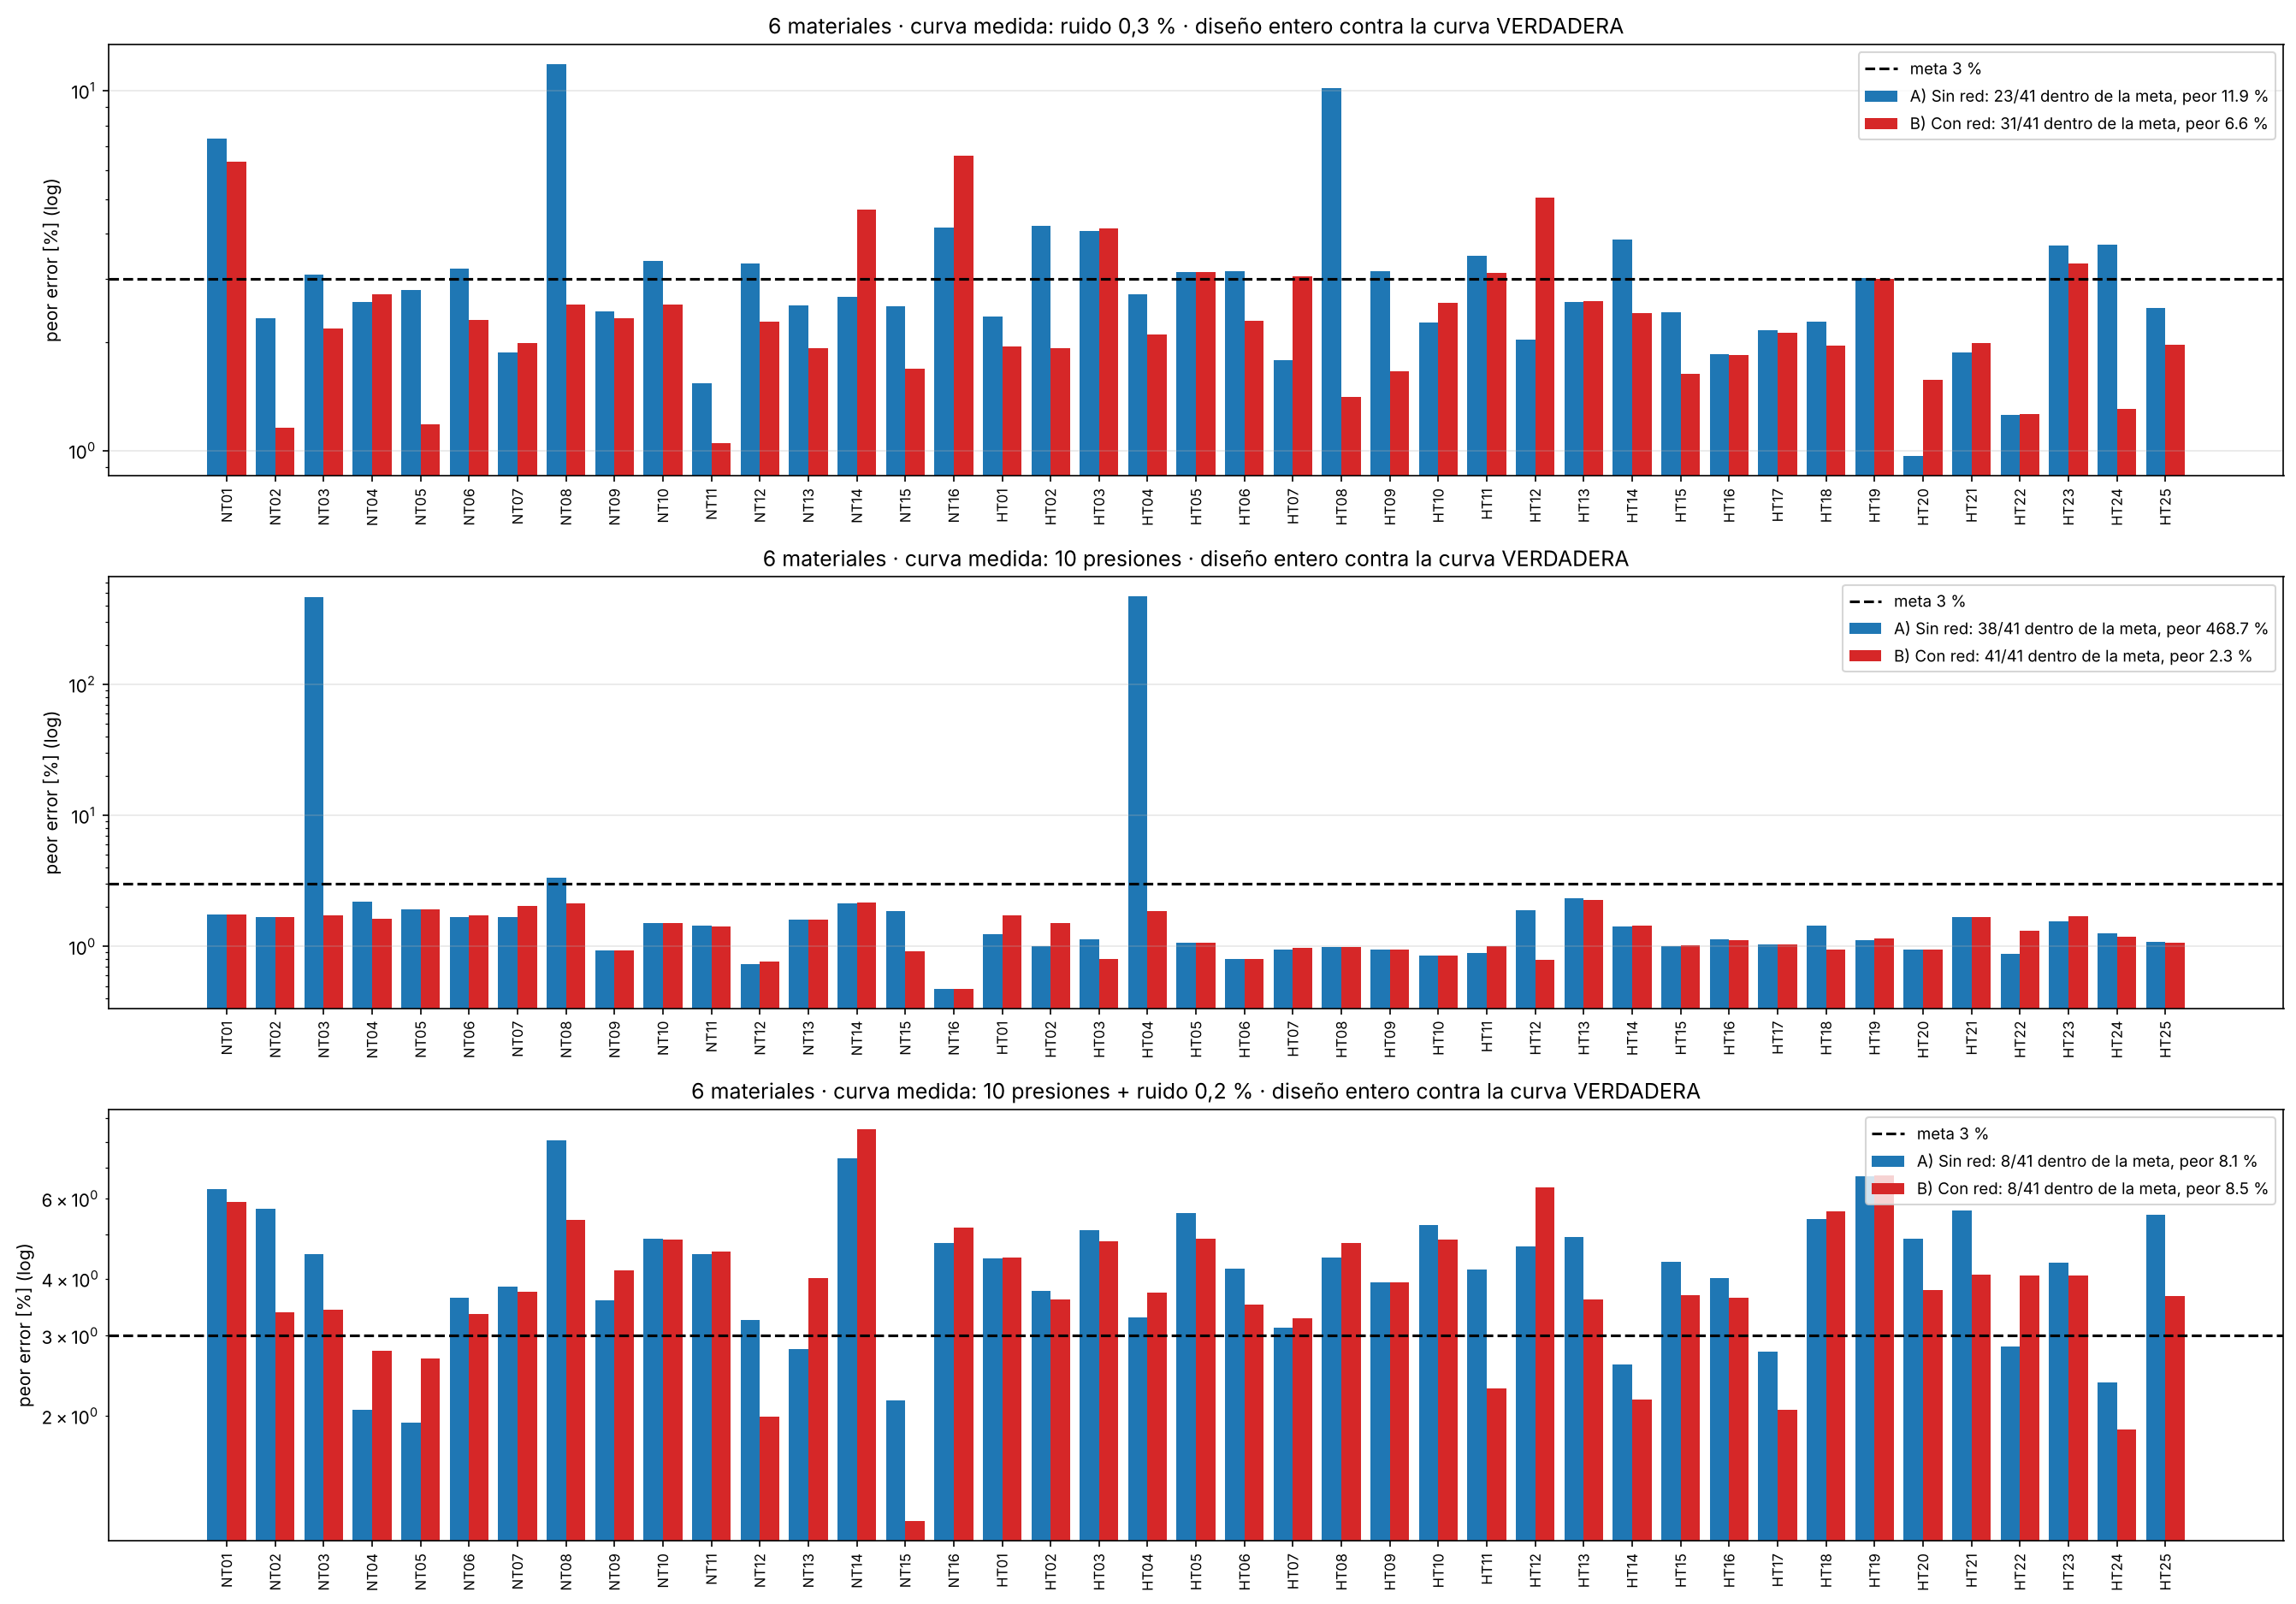
\includegraphics[width=\textwidth]{curvas_medidas_v47_6.png}
\caption{6 materials, measured curves: worst error of each subject against the true curve (logarithmic scale; blue, linear LS initialization; red, network initialization; dotted, target).}\label{fig:med47}\end{figure}

\paragraph{Against which curve to choose the laminae.} If step 3 chooses the laminae against the curve as measured, it chases the worst point, which with noise is a noise spike (Fig.~\ref{fig:suave}). Against the fitted curve of step 2, with 0.3\,\% noise and network initialization, 31 subjects meet the target instead of 10 (6 materials) and 32 instead of 5 (5 materials); the cost with clean curves is 0.2 points of median.

\begin{figure}[H]\centering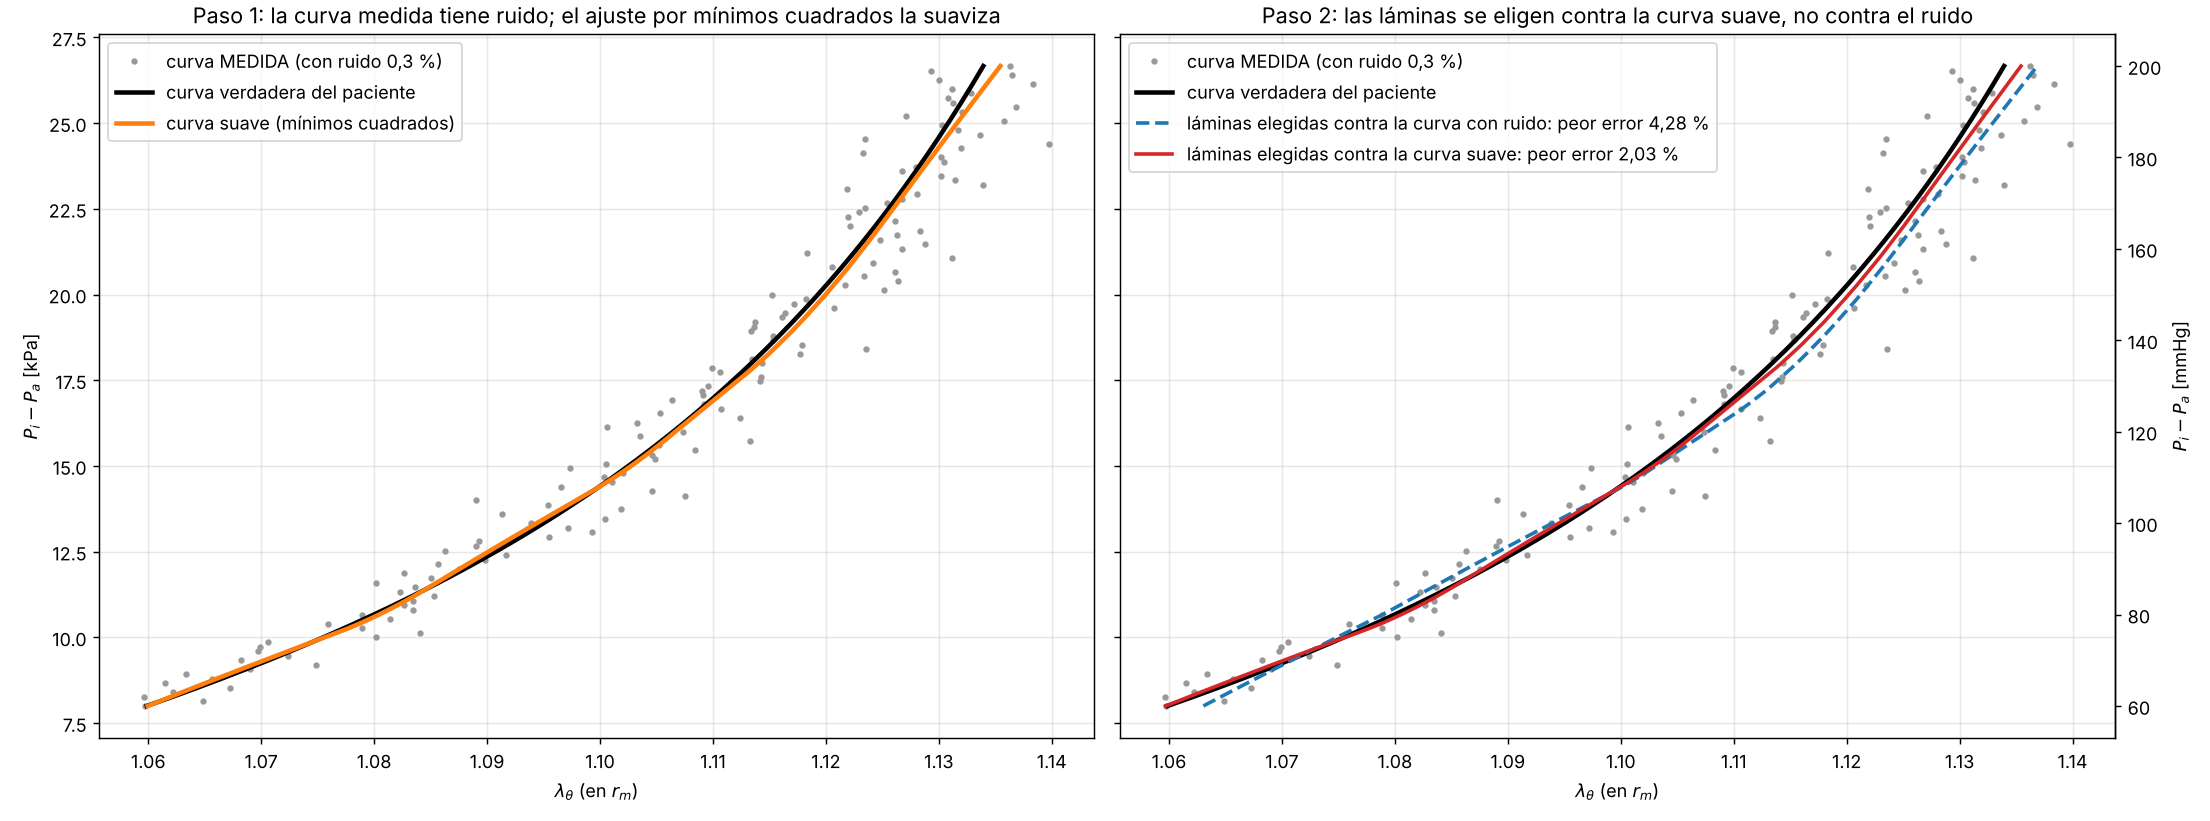
\includegraphics[width=\textwidth]{suavizado_sin_titulo.png}
\caption{Subject NT11, 6 materials, 0.3\,\% noise. Left: the curve fitted in step 2 (orange) passes through the middle of the measurement (gray). Right: laminae chosen against the measured curve ($e_{\max}=4.28$\,\%) and against the fitted one (2.03\,\%), both evaluated against the true curve.}\label{fig:suave}\end{figure}

%=====================================================================
\section{Discussion}
\paragraph{Why two levels.} The stress--stretch curve is a property of the tissue. Working on it first makes it possible to validate each component of the method ---the basis, the fit, the rounding, the network--- against exact solutions, without the intervention of geometry or pressure, which depend on each artery and each site. The transition to the tube adds the geometry and the thick-wall assumption, but keeps the materials, the metric, the minimax criterion and the conclusion about noise.

\paragraph{Generality.} What is validated at the first level is not specific to the carotid artery: the fiber-like materials, the basis chosen over a broad space of J-shaped curves, the minimax rounding and a network that reproduces the fit on curves of a law it never saw. For another artery, the geometry, thickness and pressure window change, and these only enter at the second level; the band of curves and, if necessary, the knots are recomputed with the same procedure. The class check indicates when a curve falls outside the scope of the method. The external validation (Section~\ref{sec:externa}) confirms this with data: the basis chosen with Masson's carotid arteries reproduces, unchanged, curves of common, external and internal carotid arteries, of isolated adventitia and media--intima, of rabbit and of patients with plaque, from three different constitutive laws. What limits some in vivo curves is the lamina thickness relative to a small stress excursion, not the shape of the curve. The network generalizes to those laws within the band on which it was trained; outside it, it should be used only as a starting point, and the class check together with the $y_1$--$y_2$ band suffice to detect this.

\paragraph{The role of the neural network.} In the linear case the exact solution is immediate and the network can only imitate it, although it does so in one evaluation and generalizes. In the thick-wall case the fit is iterative, local and dependent on the starting point: the classical initialization, inherited from the linear case, ignores the stretch gradient across the thickness and, with measured curves, can lead to local minima that yield unusable designs. The network, trained on thousands of solved designs, leaves the fit close to the correct minimum. This is the idea of amortized optimization~\cite{amos}: the network does not replace the optimizer, it initializes it. Its advantage is one of robustness, clear with 6 materials and smaller with 5.

\paragraph{Why a thick wall.} The difference between the models lies in a single assumption: in a thin wall all fibers stretch equally; in a thick wall each has its own stretch, set by incompressibility. With materials that bear no load until their knot, that difference of a few hundredths decides whether a layer works. The engagement of each layer (its crimp) is as important as its thickness: between a Laplace design and a thick-wall design the thicknesses change by a few micrometers, but the outer layers engage earlier.

\paragraph{Limitations.} (1) The target curves are those of the law fitted by Masson et al., not the raw measurements, and the arterial thickness is the age- and sex-specific reference value. (2) The materials are ideal (truncated lines of constant stiffness); the graft has neither axial extension nor residual stresses, and viscoelasticity and fatigue are not considered. (3) The integer search in the thick-wall case is heuristic: it stays within half a point of the optimum in a neighborhood of $\pm2$ laminae, but the global optimum was not proven; a single noise realization per subject and case was used. (4) The prestretch $\delta$ and the per-layer crimp are manufacturing variables that must be validated. (5) There is no experimental validation.

%=====================================================================
\section{Conclusions}
\begin{enumerate}
\item A graft made of layers of fiber-like materials (truncated lines), with a basis chosen once for the whole population, reproduces the stress--stretch curve of 41 human carotid arteries and of 22\,500 synthetic curves. With 6 materials and integer laminae by minimax, all 41 subjects meet the 3\,\% target.
\item Without any change, the same basis reproduces 327 curves from four other studies (Sommer and Holzapfel, Holzapfel et al., Liu et al., Kamenskiy et al.): worst error of 2.83\,\% with real-valued amounts and, at physiological stresses, 100\,\% within the target with integer laminae. The method does not depend on the artery with which it was built; for in vivo curves with a small stress excursion, the limit is the lamina thickness.
\item In the linear case, the exact method is least squares plus integer minimax (integer linear programming). The neural network reproduces it in one evaluation and generalizes to an unseen constitutive law (excess of 2.8 to 4.6\,\%), but does not improve on it.
\item At the tube level the design must be carried out with the thick-walled model: designed with Laplace's law, no subject meets the target once manufactured; with the thick-walled model, 40--41 of 41 do. The problem is a nonlinear integer one.
\item The three-step procedure ---initialization, nonlinear least squares and integer laminae by minimax against the fitted curve--- meets the target in 40--41 of 41 subjects with clean curves, in less than half a second per subject.
\item In the thick-wall case, the network as a starting point avoids the local minima that, with measured curves, produce unusable designs (worst case from 468.7 to 2.3\,\%) and increases the number of subjects within the target under noise. This is the justified role of the network: to initialize the optimizer, not to replace it.
\end{enumerate}
\paragraph{Next steps.} Test the method with raw measured curves of other arteries; test real materials to replace the ideal lines and validate crimp as a manufacturing variable; use each subject's measured thickness and pressure; and manufacture and test a graft.

%=====================================================================
\appendix
\section{Parameters of the 41 subjects}\label{sec:anexo}
\begin{table}[H]\centering\scriptsize
\caption{Parameters of Masson et al.~\cite{masson} (their Tables 2 and 4). $^\dagger$: subject held out for testing.}\label{tab:masson}
\resizebox{\textwidth}{!}{%
\begin{tabular}{lcccccccccccccccc}\toprule
Subject & Age & Sex & $R_m$ & $\Theta_0$ & $\lambda_z$ & $c$ & $c_1$ & $c_2$ & $c_1^{\mathrm{circ}}$ & $c_2^{\mathrm{circ}}$ & $\alpha$ & $T_m$ & $\lambda_0$ & $\lambda_m$ & $a$ & $b$\\
 & [years] & & [mm] & [°] & & [kPa] & [kPa] & & [kPa] & & [°] & [kPa] & & & [kPa] & \\\midrule
NT01 & 62 & F & 4.26 & 128.70 & 1.11 & 29.82 & 9.44 & 14.14 & 16.13 & 15.11 & 65.74 & 39.73 & 0.960 & 1.70 & 0.122 & 3.52\\
NT02$^\dagger$ & 60 & M & 4.69 & 128.90 & 1.08 & 20.42 & 8.47 & 13.10 & 14.16 & 15.12 & 44.46 & 41.84 & 0.680 & 1.92 & 0.126 & 3.40\\
NT03 & 31 & M & 4.30 & 132.20 & 1.09 & 27.23 & 10.34 & 13.10 & 7.01 & 12.82 & 48.62 & 43.37 & 0.820 & 1.65 & 0.139 & 3.57\\
NT04 & 31 & M & 4.67 & 133.90 & 1.10 & 23.59 & 6.58 & 11.77 & 6.38 & 10.69 & 32.04 & 39.81 & 0.680 & 1.59 & 0.118 & 3.53\\
NT05 & 34 & F & 4.20 & 130.10 & 1.10 & 35.68 & 13.62 & 13.18 & 13.38 & 13.17 & 50.72 & 50.07 & 0.860 & 1.62 & 0.103 & 3.58\\
NT06 & 53 & F & 3.96 & 130.10 & 1.11 & 33.37 & 11.38 & 13.63 & 13.30 & 14.26 & 57.14 & 46.59 & 0.950 & 1.69 & 0.093 & 3.44\\
NT07 & 21 & F & 3.83 & 132.00 & 1.10 & 44.28 & 21.79 & 13.17 & 8.27 & 12.73 & 51.15 & 53.58 & 0.920 & 1.62 & 0.111 & 3.58\\
NT08$^\dagger$ & 25 & M & 4.86 & 133.20 & 1.07 & 23.25 & 6.34 & 12.93 & 8.11 & 13.17 & 42.93 & 31.90 & 0.820 & 1.77 & 0.173 & 3.57\\
NT09 & 42 & F & 4.51 & 129.50 & 1.10 & 34.90 & 16.14 & 13.58 & 19.64 & 13.89 & 57.21 & 47.01 & 0.930 & 1.65 & 0.084 & 3.55\\
NT10$^\dagger$ & 55 & M & 4.77 & 129.10 & 1.10 & 38.57 & 36.31 & 13.31 & 56.88 & 13.61 & 54.22 & 46.36 & 0.890 & 1.66 & 0.006 & 3.75\\
NT11$^\dagger$ & 64 & M & 5.57 & 129.50 & 1.10 & 34.89 & 40.16 & 13.45 & 66.88 & 13.53 & 54.54 & 41.12 & 0.850 & 1.79 & 0.005 & 3.23\\
NT12 & 60 & F & 4.88 & 130.10 & 1.09 & 33.94 & 10.78 & 13.95 & 12.79 & 15.42 & 60.97 & 45.77 & 0.930 & 1.73 & 0.099 & 3.37\\
NT13 & 61 & F & 4.92 & 130.60 & 1.09 & 35.15 & 17.69 & 13.43 & 18.40 & 13.22 & 55.04 & 45.59 & 0.940 & 1.66 & 0.085 & 3.51\\
NT14 & 39 & F & 3.54 & 131.50 & 1.09 & 28.97 & 8.22 & 13.13 & 19.02 & 13.16 & 50.22 & 41.30 & 0.890 & 1.67 & 0.105 & 3.53\\
NT15 & 58 & F & 3.92 & 132.40 & 1.08 & 26.71 & 15.79 & 13.36 & 16.68 & 13.11 & 53.60 & 35.32 & 0.950 & 1.71 & 0.166 & 3.60\\
NT16 & 60 & M & 5.72 & 129.70 & 1.10 & 27.79 & 28.23 & 13.46 & 57.77 & 13.63 & 55.73 & 36.50 & 1.05 & 1.77 & 0.141 & 3.58\\
HT01 & 68 & M & 4.96 & 130.90 & 1.10 & 35.91 & 12.57 & 14.08 & 15.52 & 14.91 & 67.18 & 48.42 & 0.990 & 1.66 & 0.098 & 3.50\\
HT02 & 54 & M & 4.93 & 129.80 & 1.10 & 38.20 & 16.40 & 13.20 & 16.44 & 13.20 & 51.11 & 52.44 & 0.860 & 1.62 & 0.137 & 3.58\\
HT03$^\dagger$ & 64 & F & 4.87 & 129.50 & 1.10 & 36.01 & 14.55 & 13.96 & 18.35 & 14.48 & 62.66 & 47.02 & 1.00 & 1.74 & 0.113 & 3.62\\
HT04 & 58 & F & 4.57 & 131.20 & 1.09 & 22.42 & 8.57 & 13.03 & 6.43 & 13.36 & 46.38 & 38.53 & 0.810 & 1.68 & 0.099 & 3.51\\
HT05$^\dagger$ & 62 & F & 4.78 & 130.10 & 1.10 & 48.19 & 35.06 & 13.23 & 43.19 & 13.03 & 53.24 & 52.86 & 0.910 & 1.63 & 0.033 & 3.56\\
HT06 & 66 & F & 5.06 & 129.10 & 1.10 & 39.78 & 37.75 & 13.35 & 60.89 & 13.45 & 56.01 & 46.44 & 0.910 & 1.64 & 0.004 & 3.54\\
HT07 & 54 & F & 4.30 & 129.60 & 1.11 & 50.45 & 25.51 & 13.32 & 39.43 & 13.24 & 53.47 & 64.91 & 0.930 & 1.66 & 0.078 & 3.72\\
HT08 & 63 & F & 4.44 & 129.00 & 1.10 & 34.44 & 30.62 & 13.29 & 60.33 & 13.21 & 54.67 & 44.94 & 0.930 & 1.65 & 0.084 & 3.56\\
HT09 & 68 & M & 5.09 & 128.20 & 1.12 & 51.48 & 33.77 & 13.17 & 44.26 & 13.49 & 51.83 & 66.41 & 0.840 & 1.62 & 0.023 & 3.55\\
HT10 & 55 & F & 4.30 & 129.00 & 1.10 & 37.04 & 12.32 & 14.13 & 15.04 & 14.93 & 65.14 & 48.19 & 1.04 & 1.71 & 0.114 & 3.47\\
HT11 & 69 & M & 5.54 & 131.20 & 1.08 & 29.64 & 9.76 & 13.23 & 9.10 & 15.12 & 48.16 & 37.83 & 0.830 & 1.74 & 0.115 & 3.59\\
HT12 & 54 & M & 5.43 & 131.80 & 1.09 & 32.23 & 17.81 & 13.35 & 14.03 & 12.15 & 53.73 & 44.93 & 0.920 & 1.65 & 0.090 & 3.58\\
HT13$^\dagger$ & 61 & M & 5.17 & 128.40 & 1.11 & 30.45 & 15.87 & 13.08 & 23.03 & 13.84 & 47.86 & 52.58 & 0.750 & 1.61 & 0.009 & 3.49\\
HT14$^\dagger$ & 60 & M & 4.64 & 129.90 & 1.10 & 30.43 & 13.74 & 13.45 & 18.01 & 13.35 & 54.90 & 42.43 & 0.910 & 1.66 & 0.088 & 3.52\\
HT15 & 53 & M & 4.65 & 130.40 & 1.10 & 40.83 & 28.98 & 13.36 & 31.16 & 12.62 & 54.44 & 49.57 & 0.930 & 1.65 & 0.085 & 3.63\\
HT16 & 54 & M & 4.71 & 129.60 & 1.10 & 45.26 & 29.27 & 14.00 & 33.48 & 14.82 & 67.16 & 67.68 & 1.02 & 1.65 & 0.039 & 3.52\\
HT17 & 53 & M & 5.04 & 130.00 & 1.10 & 37.25 & 39.18 & 13.24 & 66.29 & 13.15 & 54.90 & 48.26 & 0.910 & 1.64 & 0.099 & 3.60\\
HT18 & 52 & M & 4.92 & 129.70 & 1.10 & 29.28 & 10.50 & 13.21 & 19.76 & 13.39 & 50.96 & 46.42 & 0.850 & 1.63 & 0.094 & 3.56\\
HT19$^\dagger$ & 57 & F & 4.27 & 130.30 & 1.10 & 33.49 & 14.47 & 13.22 & 17.35 & 13.27 & 53.18 & 46.18 & 0.900 & 1.64 & 0.097 & 3.55\\
HT20 & 61 & F & 5.14 & 129.20 & 1.10 & 40.09 & 15.72 & 14.09 & 16.78 & 14.83 & 65.17 & 53.40 & 1.04 & 1.70 & 0.100 & 3.47\\
HT21 & 57 & F & 4.88 & 129.90 & 1.10 & 35.31 & 14.57 & 13.26 & 15.58 & 13.30 & 52.07 & 48.97 & 0.870 & 1.63 & 0.094 & 3.57\\
HT22 & 44 & F & 4.17 & 131.00 & 1.10 & 55.25 & 35.78 & 13.23 & 19.51 & 12.55 & 52.36 & 59.58 & 0.930 & 1.61 & 0.097 & 3.61\\
HT23 & 51 & M & 4.83 & 130.60 & 1.08 & 30.77 & 12.80 & 13.60 & 41.10 & 14.20 & 49.79 & 41.06 & 0.870 & 1.90 & 0.094 & 3.56\\
HT24$^\dagger$ & 65 & M & 4.57 & 129.60 & 1.10 & 38.91 & 25.76 & 13.20 & 35.01 & 13.20 & 51.94 & 50.28 & 0.870 & 1.62 & 0.043 & 3.58\\
HT25 & 67 & F & 4.72 & 129.20 & 1.10 & 40.29 & 31.78 & 13.75 & 60.40 & 14.29 & 63.50 & 46.06 & 1.03 & 1.72 & 0.025 & 3.46\\
\bottomrule\end{tabular}}
\end{table}


\section{Worked example of a thick-wall design}\label{sec:ejemplo}
This appendix shows, with numbers that can be checked with a calculator, the ideas used in Section~\ref{sec:aplicacion}: the graft reproduces the behavior of the artery with layers of different materials; each fiber of a thick wall stretches differently; pressure is the sum of the contributions of thin slices; the position of each layer changes what it contributes; and the prestretch $\delta$ shifts all the knots. To keep the calculations short, the tube is closed, without residual stresses and without axial extension, and the knot of each material is applied directly to the local stretch of each slice (in the complete model the knot is defined at the mid-wall and translated to each layer by incompressibility, Eq.~\ref{eq:incomp}).

\subsection{The artery and the graft}
\begin{figure}[H]\centering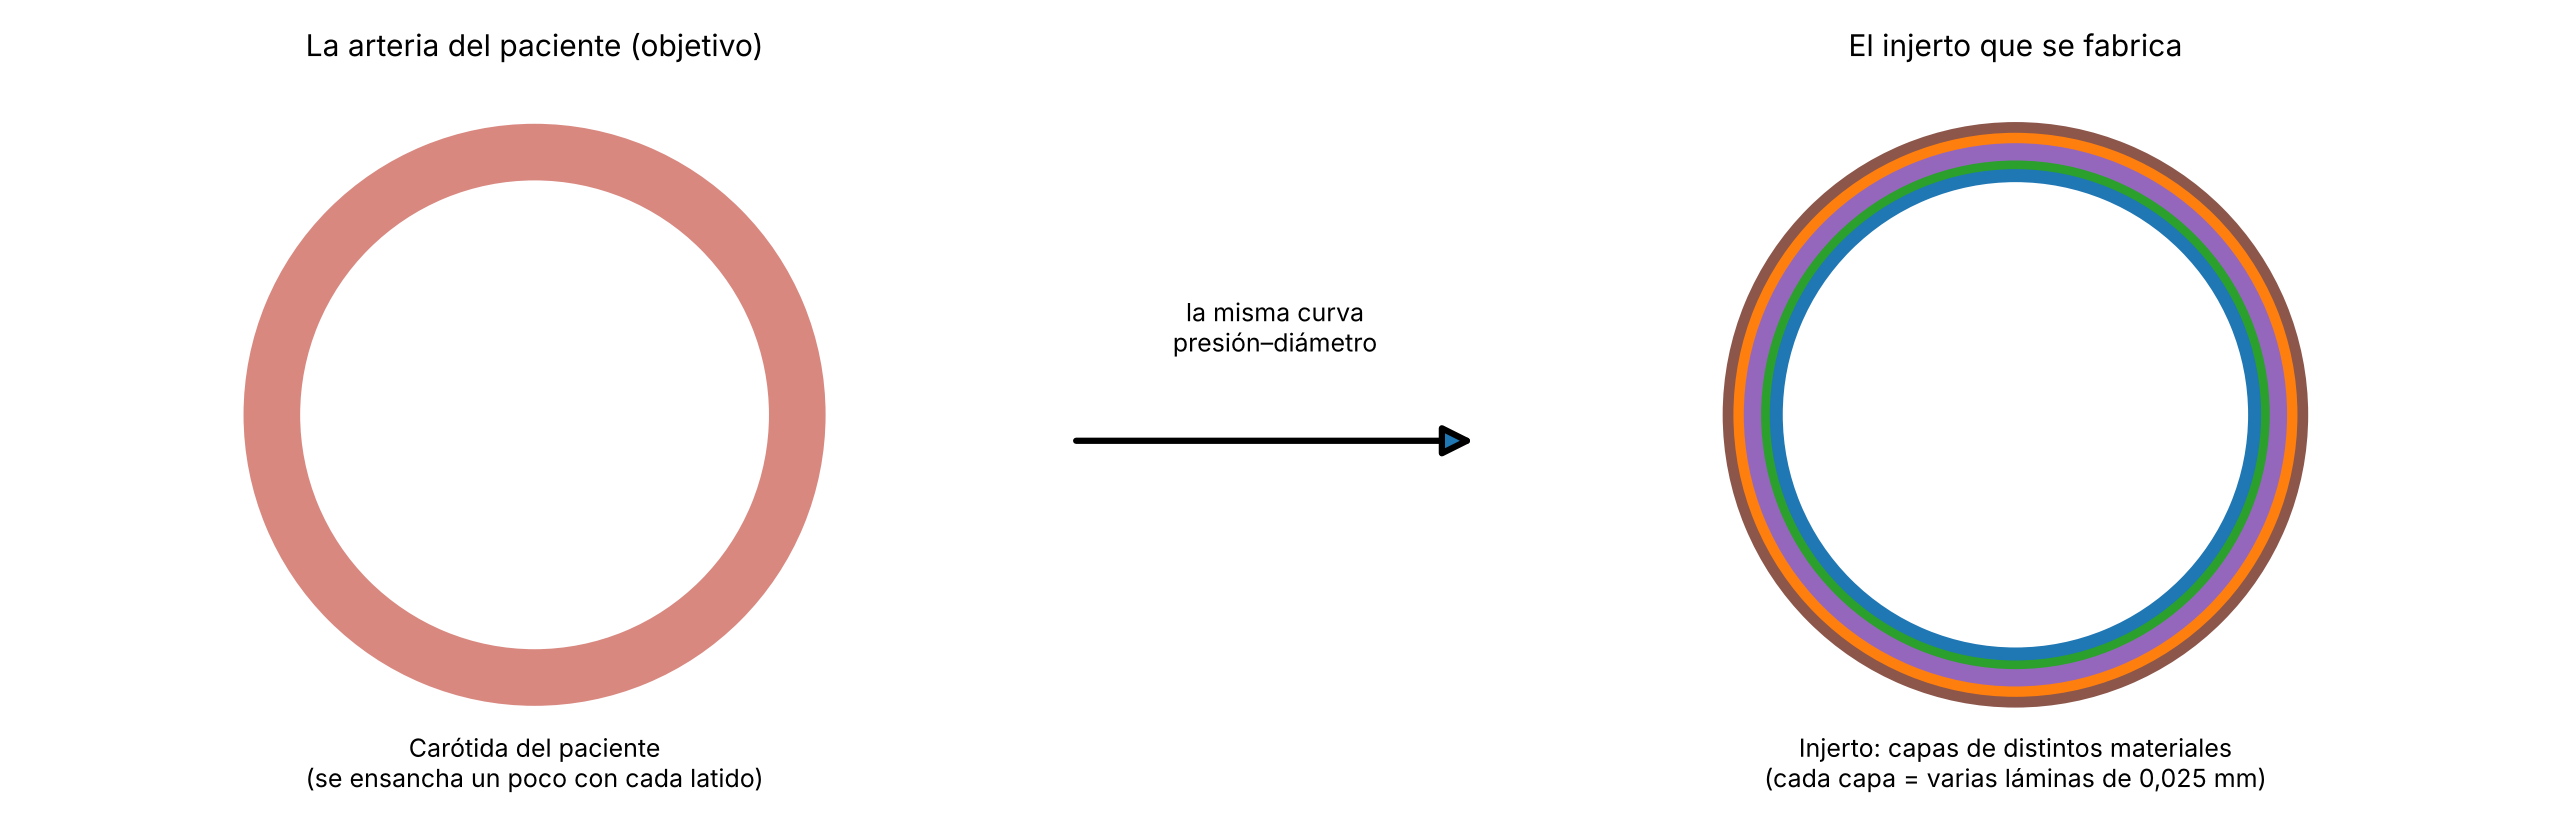
\includegraphics[width=0.85\textwidth]{d12_objetivo_v2.png}
\caption{The patient's carotid artery (left) and the graft (right), made of layers of different materials, each layer with an integer number of laminae. The goal is for the graft to have the same pressure--diameter curve as the artery: both should widen equally with pressure.}\end{figure}

\subsection{Incompressibility: the ring area does not change}
Tissue is mostly water: it deforms without changing volume. If the tube does not extend axially, the ring area is the same before and after inflation:
\[
\pi\,(R_o^2-R_i^2)=\pi\,(r_o^2-r_i^2)\qquad\Longrightarrow\qquad r=\sqrt{r_i^2+R^2-R_i^2}\quad\text{for any wall radius }R.
\]
Example tube: unpressurized from $R_i=3.0$ to $R_o=3.6$\,mm; under pressure the inner surface reaches $r_i=3.3$\,mm. Then $r=\sqrt{1.89+R^2}$ (because $3.3^2-3.0^2=1.89$) and $r_o=\sqrt{14.85}=3.854$\,mm. The inner surface stretches $3.3/3.0=1.100$ and the outer one $3.854/3.6=1.070$ (Fig.~\ref{fig:fibra}): \textbf{in a thick wall there is no single stretch}.
\begin{figure}[H]\centering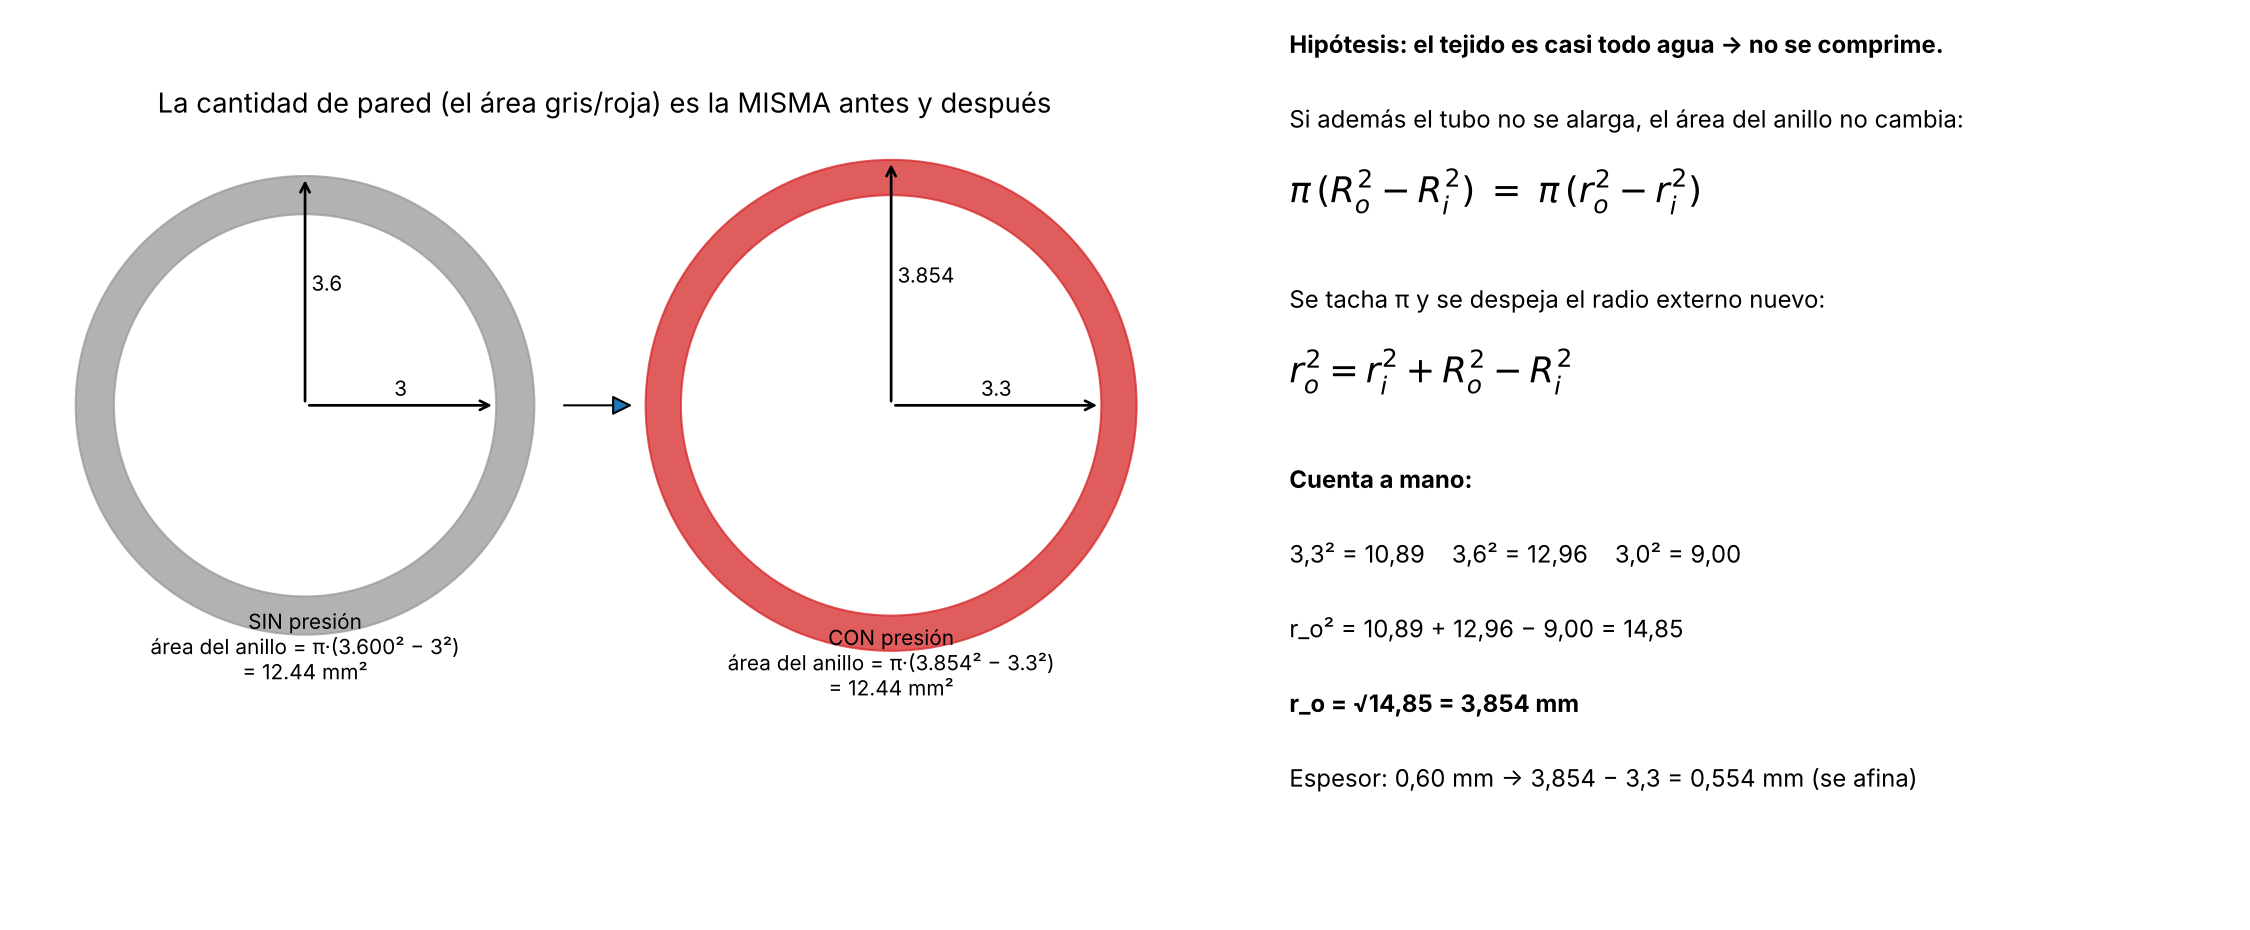
\includegraphics[width=0.9\textwidth]{d5_area_constante.png}
\caption{The ring area (gray unpressurized, red pressurized) is the same: $\pi(3.6^2-3.0^2)=\pi(3.854^2-3.3^2)=12.44$\,mm$^2$.}\end{figure}

\subsection{The thick wall as a stack of thin walls}
The wall is cut into thin slices. Each slice is a thin wall, with its own stretch $\lambda=r_c/R_c$ (at its center), and contributes $\sigma\,\Delta r/r_c$ (Laplace); the pressure is the sum, which in the limit is the integral of Eq.~\eqref{eq:pgruesa}.
\begin{figure}[H]\centering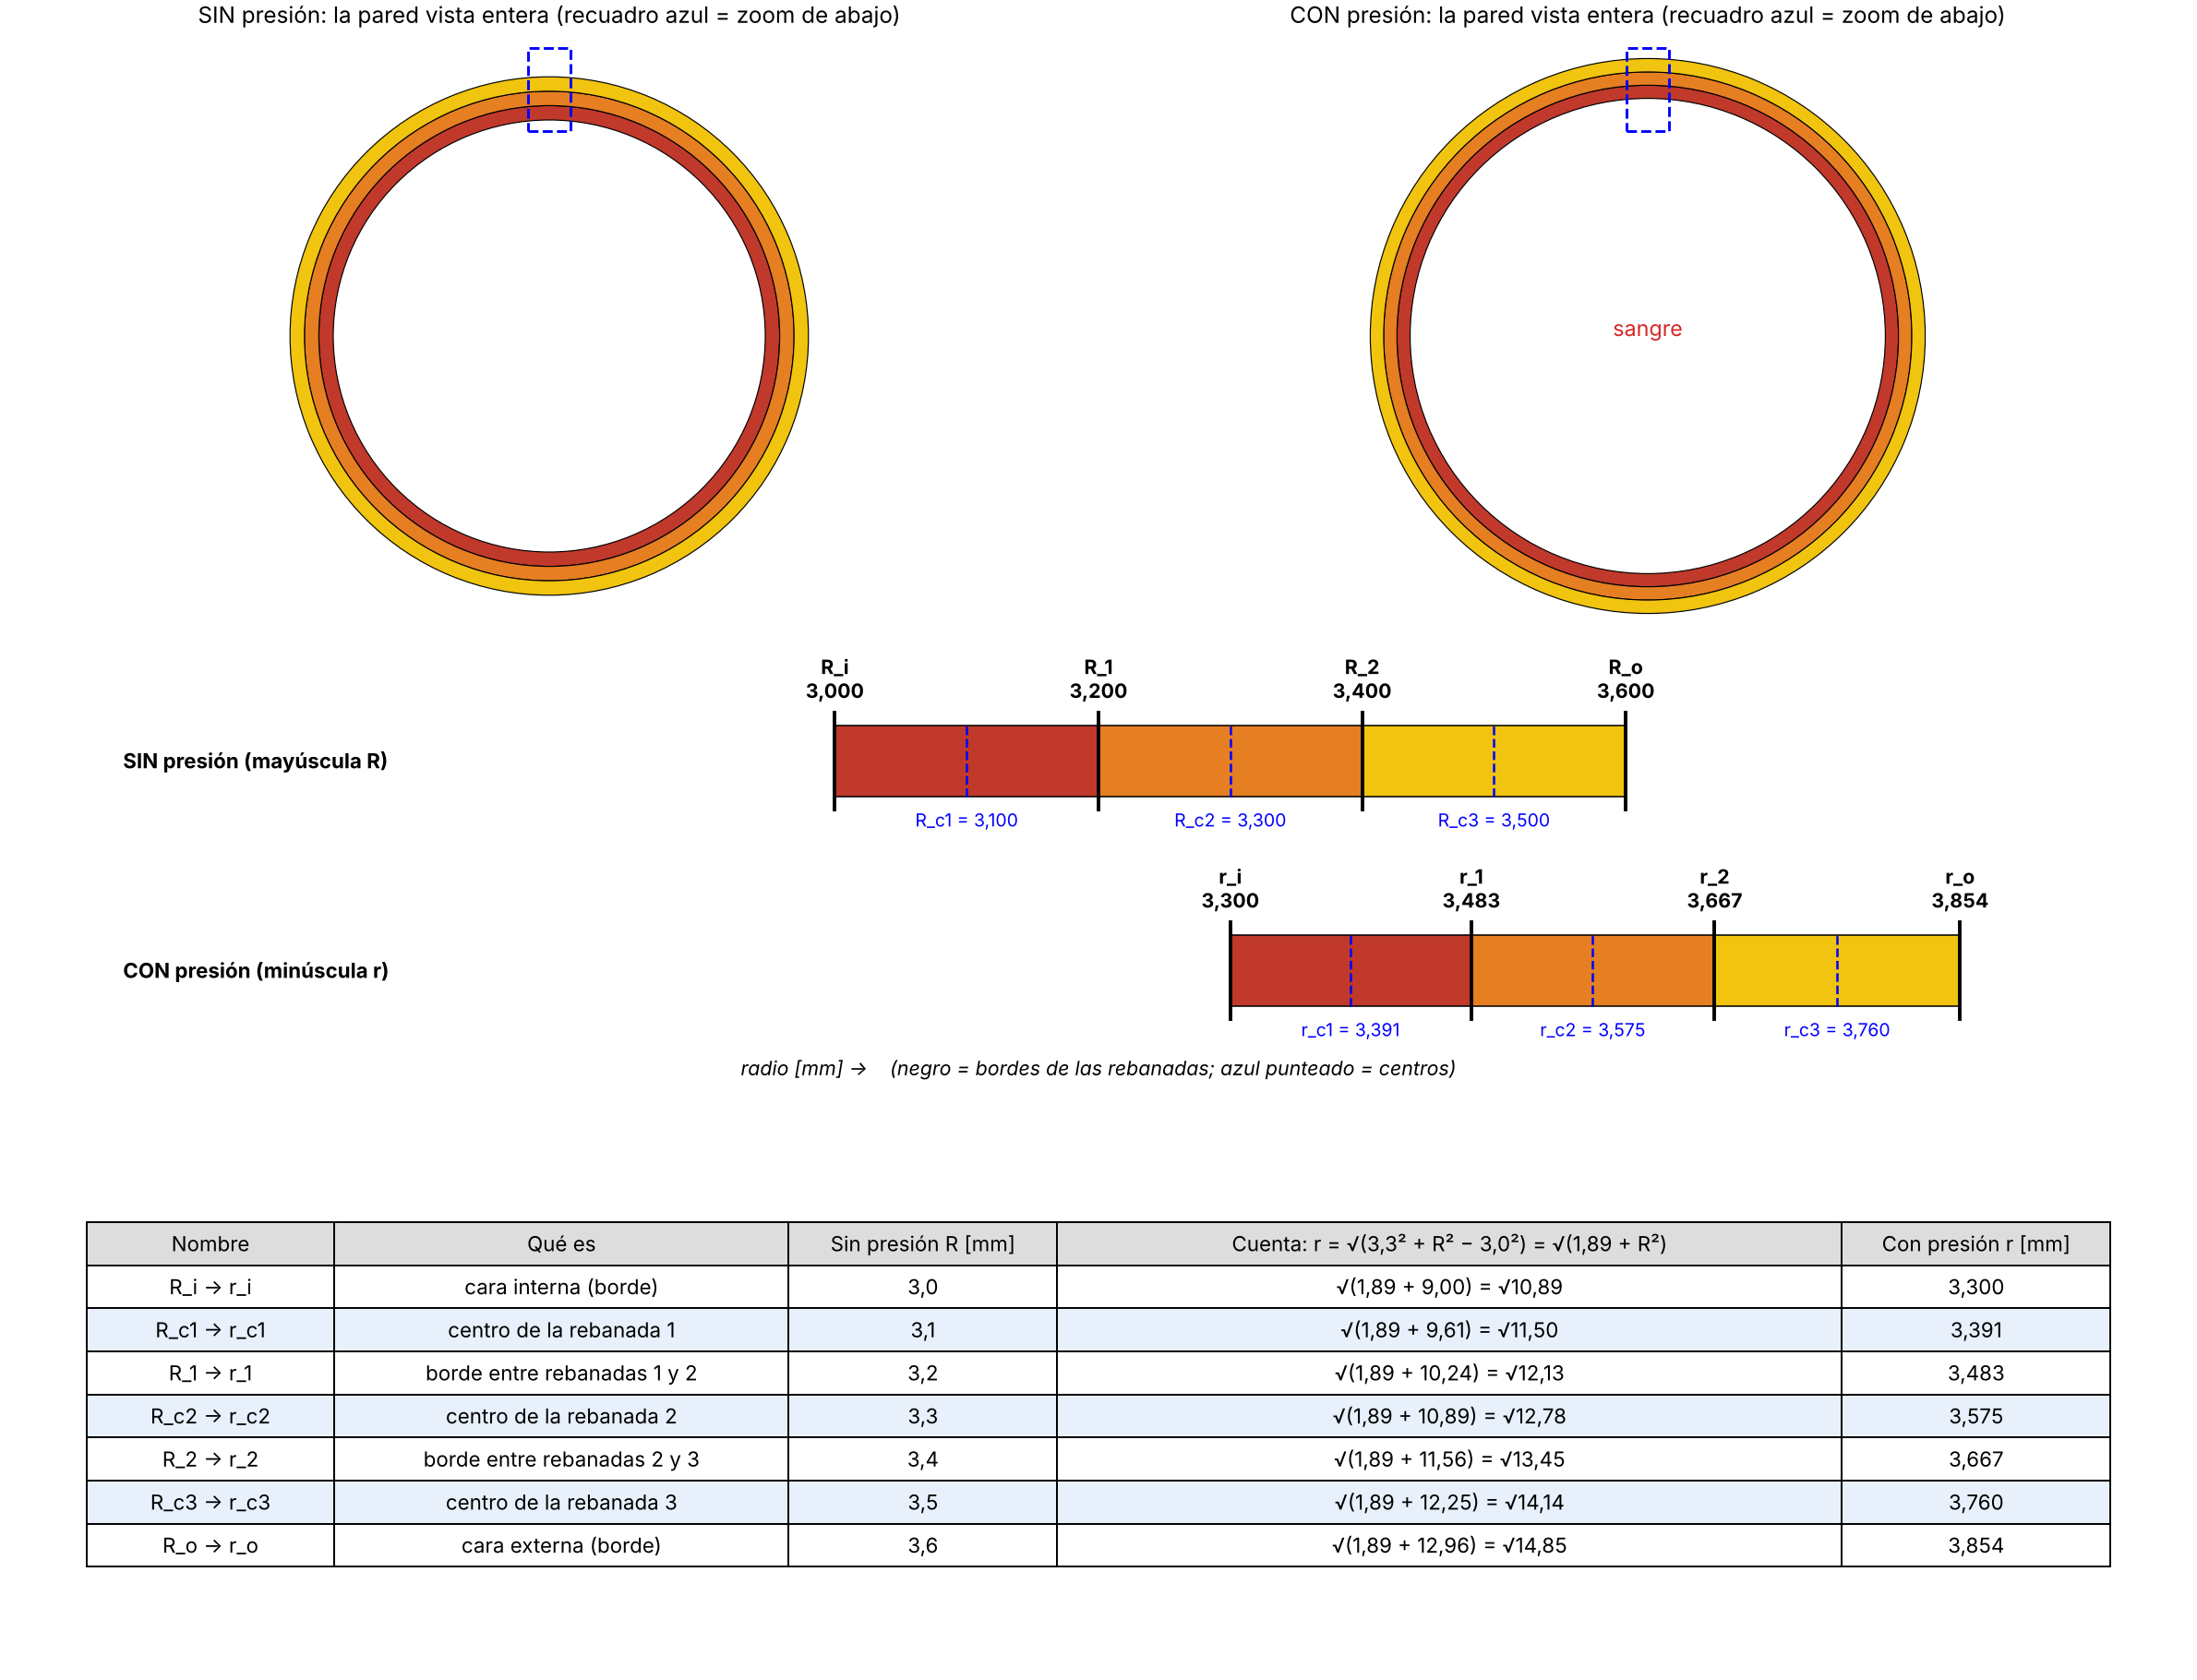
\includegraphics[width=0.9\textwidth]{d15_radios_rebanadas.png}
\caption{The example tube in 3 slices: boundaries (black) and centers (blue), unpressurized ($R$) and pressurized ($r=\sqrt{1.89+R^2}$).}\end{figure}
With a material without knot, $\sigma=1000\,(\lambda-1)$\,kPa:
\begin{center}\small
\begin{tabular}{lccc}\toprule
 & Slice 1 (inner) & Slice 2 & Slice 3 (outer)\\\midrule
unpressurized center $R_c$ [mm] & 3.1 & 3.3 & 3.5\\
pressurized center $r_c=\sqrt{1.89+R_c^2}$ [mm] & 3.391 & 3.575 & 3.760\\
stretch $\lambda=r_c/R_c$ & 1.094 & 1.083 & 1.074\\
stress $\sigma$ [kPa] & 93.9 & 83.3 & 74.4\\
inflated thickness $\Delta r$ [mm] & 0.183 & 0.185 & 0.186\\
contribution $\sigma\,\Delta r/r_c$ [kPa] & 5.06 & 4.30 & 3.68\\\bottomrule
\end{tabular}
\end{center}
The total pressure is $5.06+4.30+3.68=13.05$\,kPa (with thousands of slices, 13.07). The inner slice contributes more because it stretches more.
\begin{figure}[H]\centering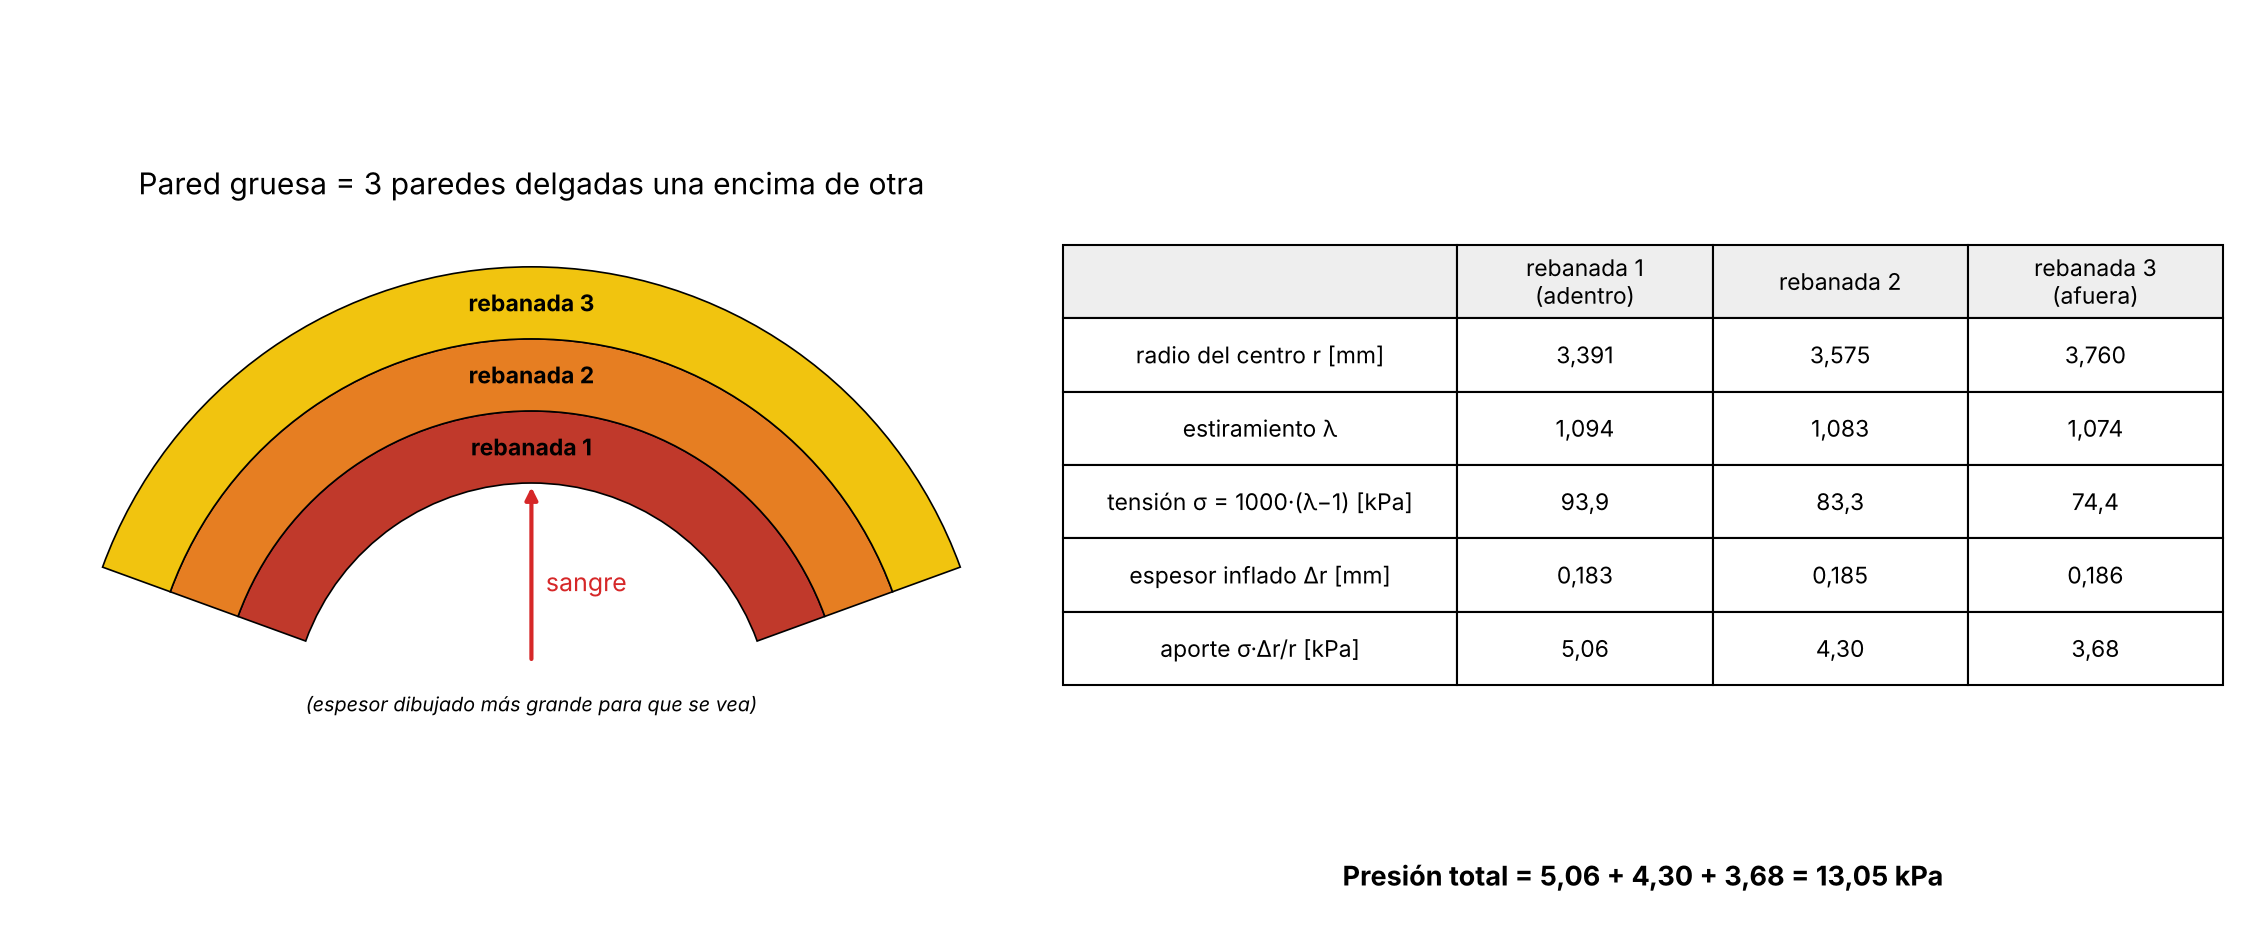
\includegraphics[width=0.55\textwidth]{d13_rebanadas.png}
\caption{Thick wall = three thin walls, one on top of the other.}\end{figure}

\subsection{In a thick wall, the position of each layer matters}
The wall now has two materials with knots, $\sigma=E\max(0,\lambda-k)$: a blue layer ($k=1.02$, $E=400$\,kPa) from 3.0 to 3.3\,mm and a green one ($k=1.08$, $E=1500$\,kPa) from 3.3 to 3.6\,mm, each cut into 3 slices.
\begin{figure}[H]\centering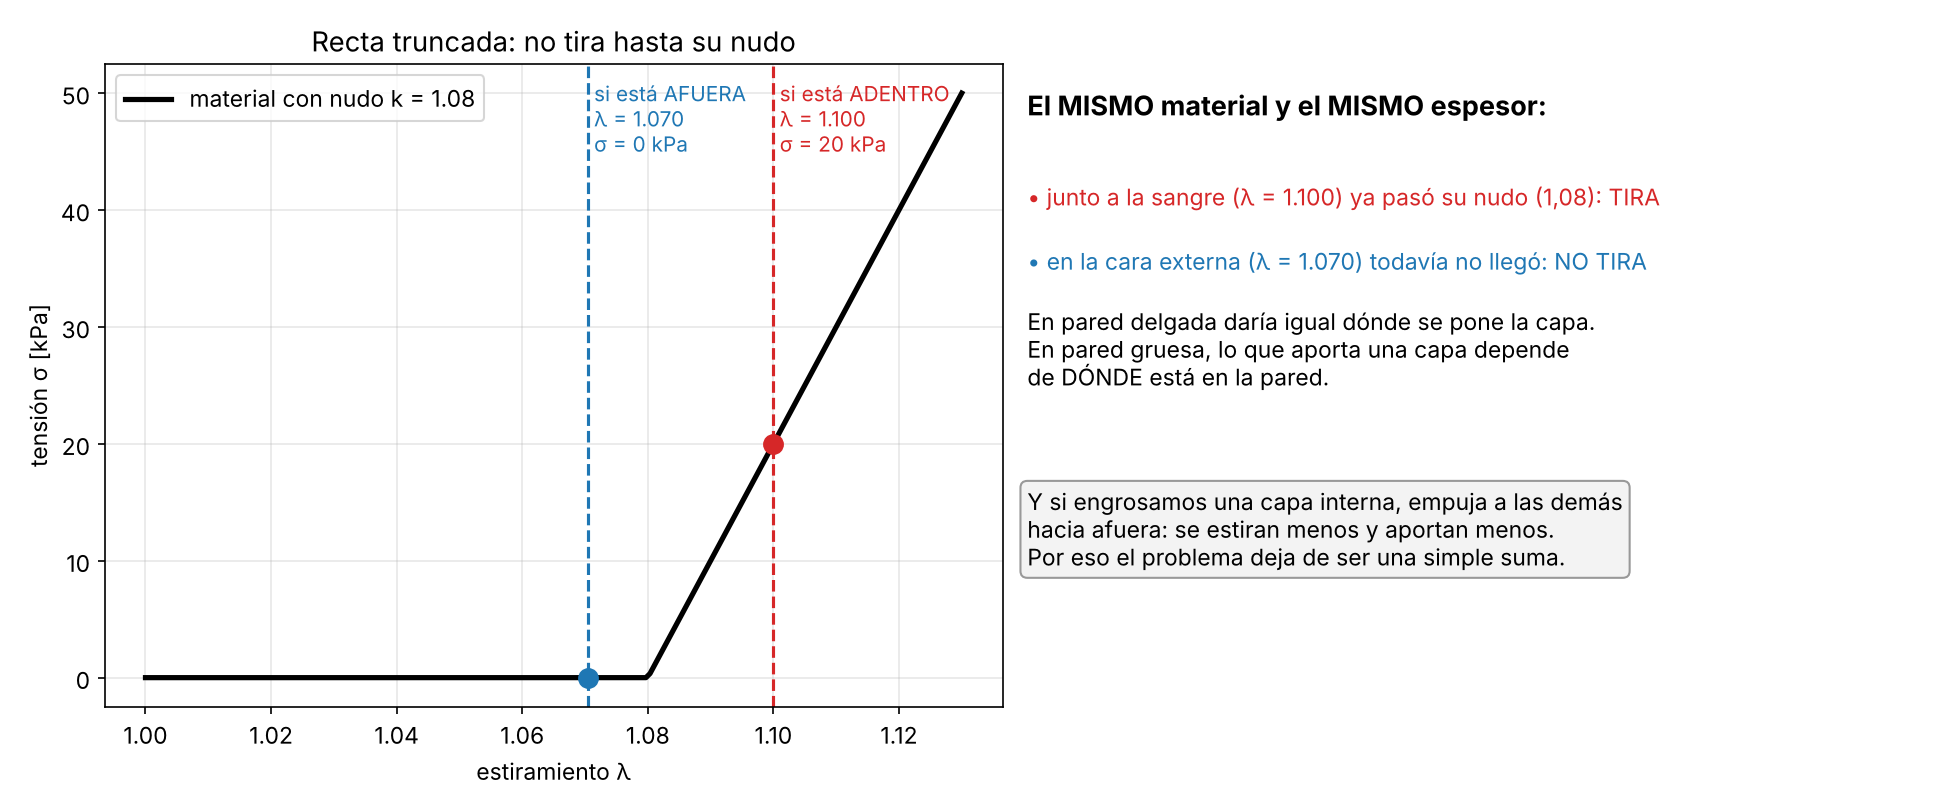
\includegraphics[width=0.9\textwidth]{d3_posicion.png}
\caption{A material with knot 1.08 (in the drawing, $E=1000$\,kPa) bears load next to the blood ($\lambda=1.100$: $\sigma=1000\times0.020=20$\,kPa) and bears no load at the outer surface ($\lambda=1.070<1.08$: $\sigma=0$). The same material and the same thickness contribute differently depending on where they are.}\end{figure}
\begin{figure}[H]\centering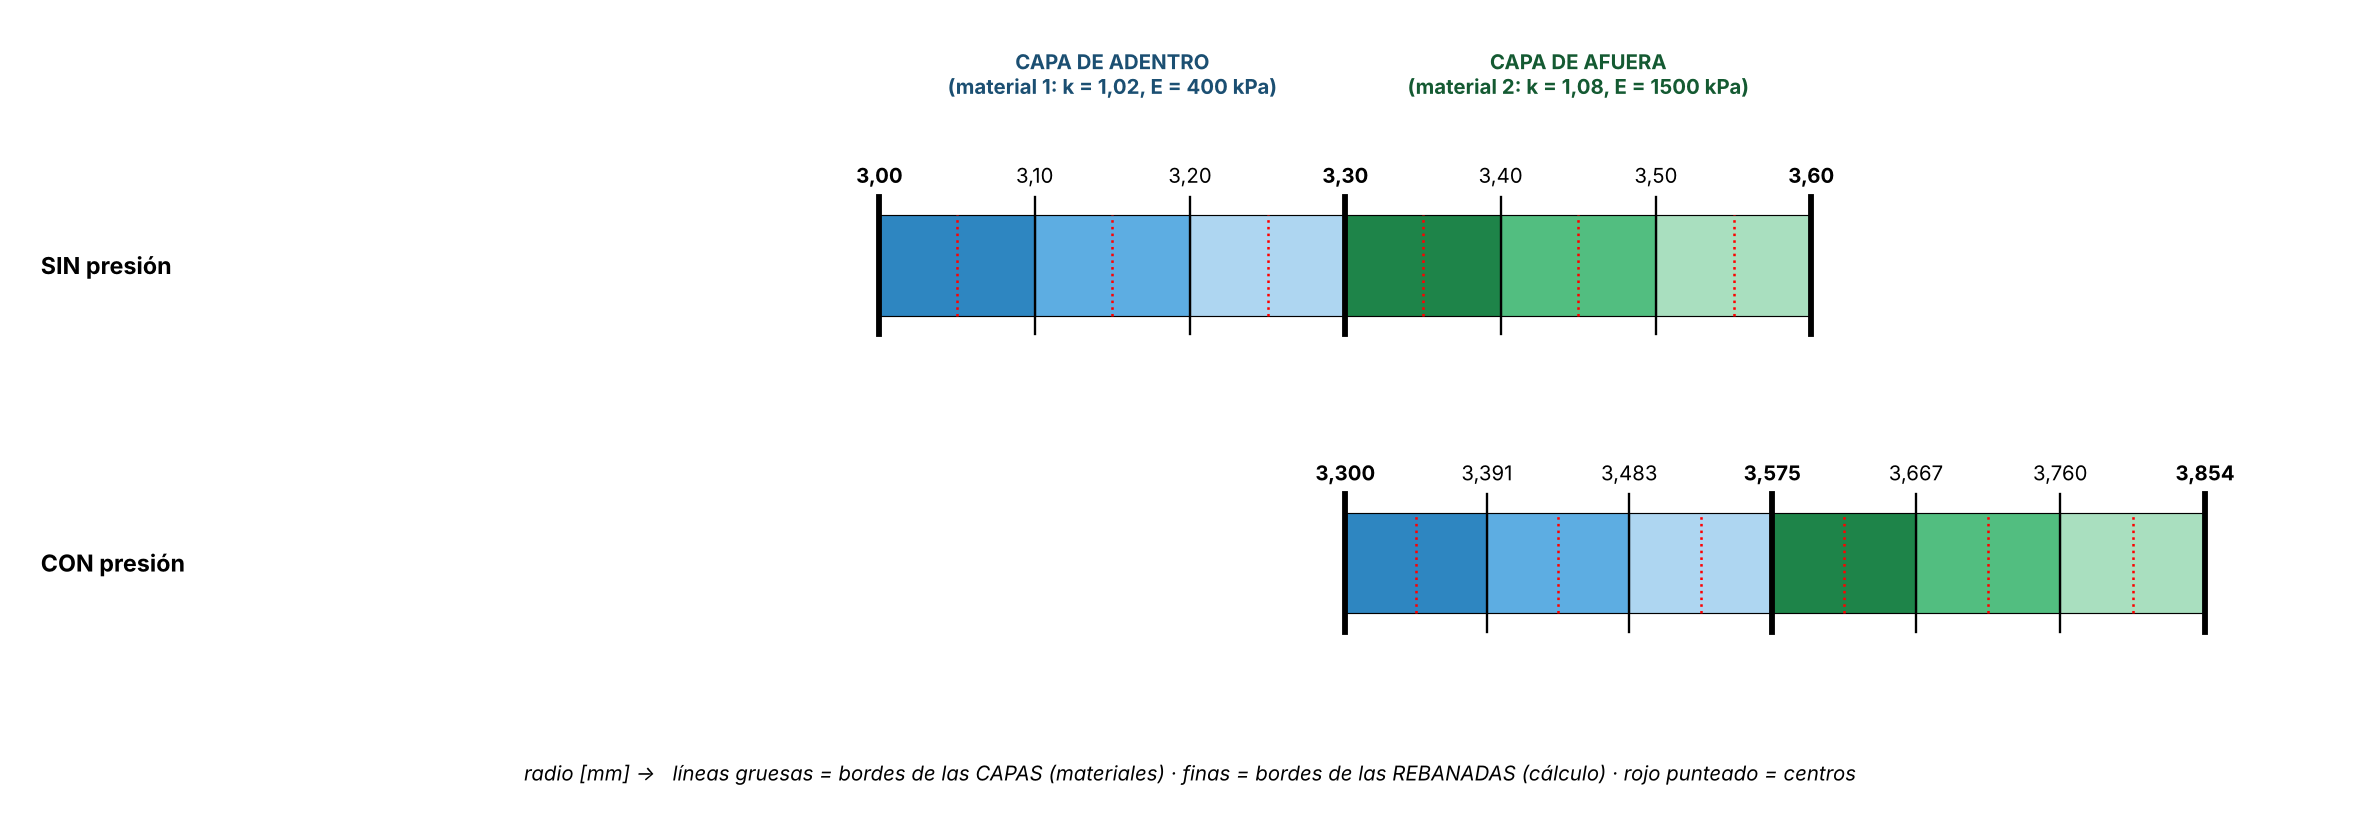
\includegraphics[width=\textwidth]{d16_dos_capas.png}
\caption{Two 0.3\,mm layers, unpressurized (top) and pressurized (bottom). The blue layer contributes $0.84+0.76+0.69=2.28$\,kPa; of the green one, only the first slice bears load ($\lambda=1.081$): 0.04\,kPa.}\end{figure}
If only the thickness of the blue layer is changed, the green one ---untouched--- changes its contribution, because it is pushed outward and stretches less:
\begin{figure}[H]\centering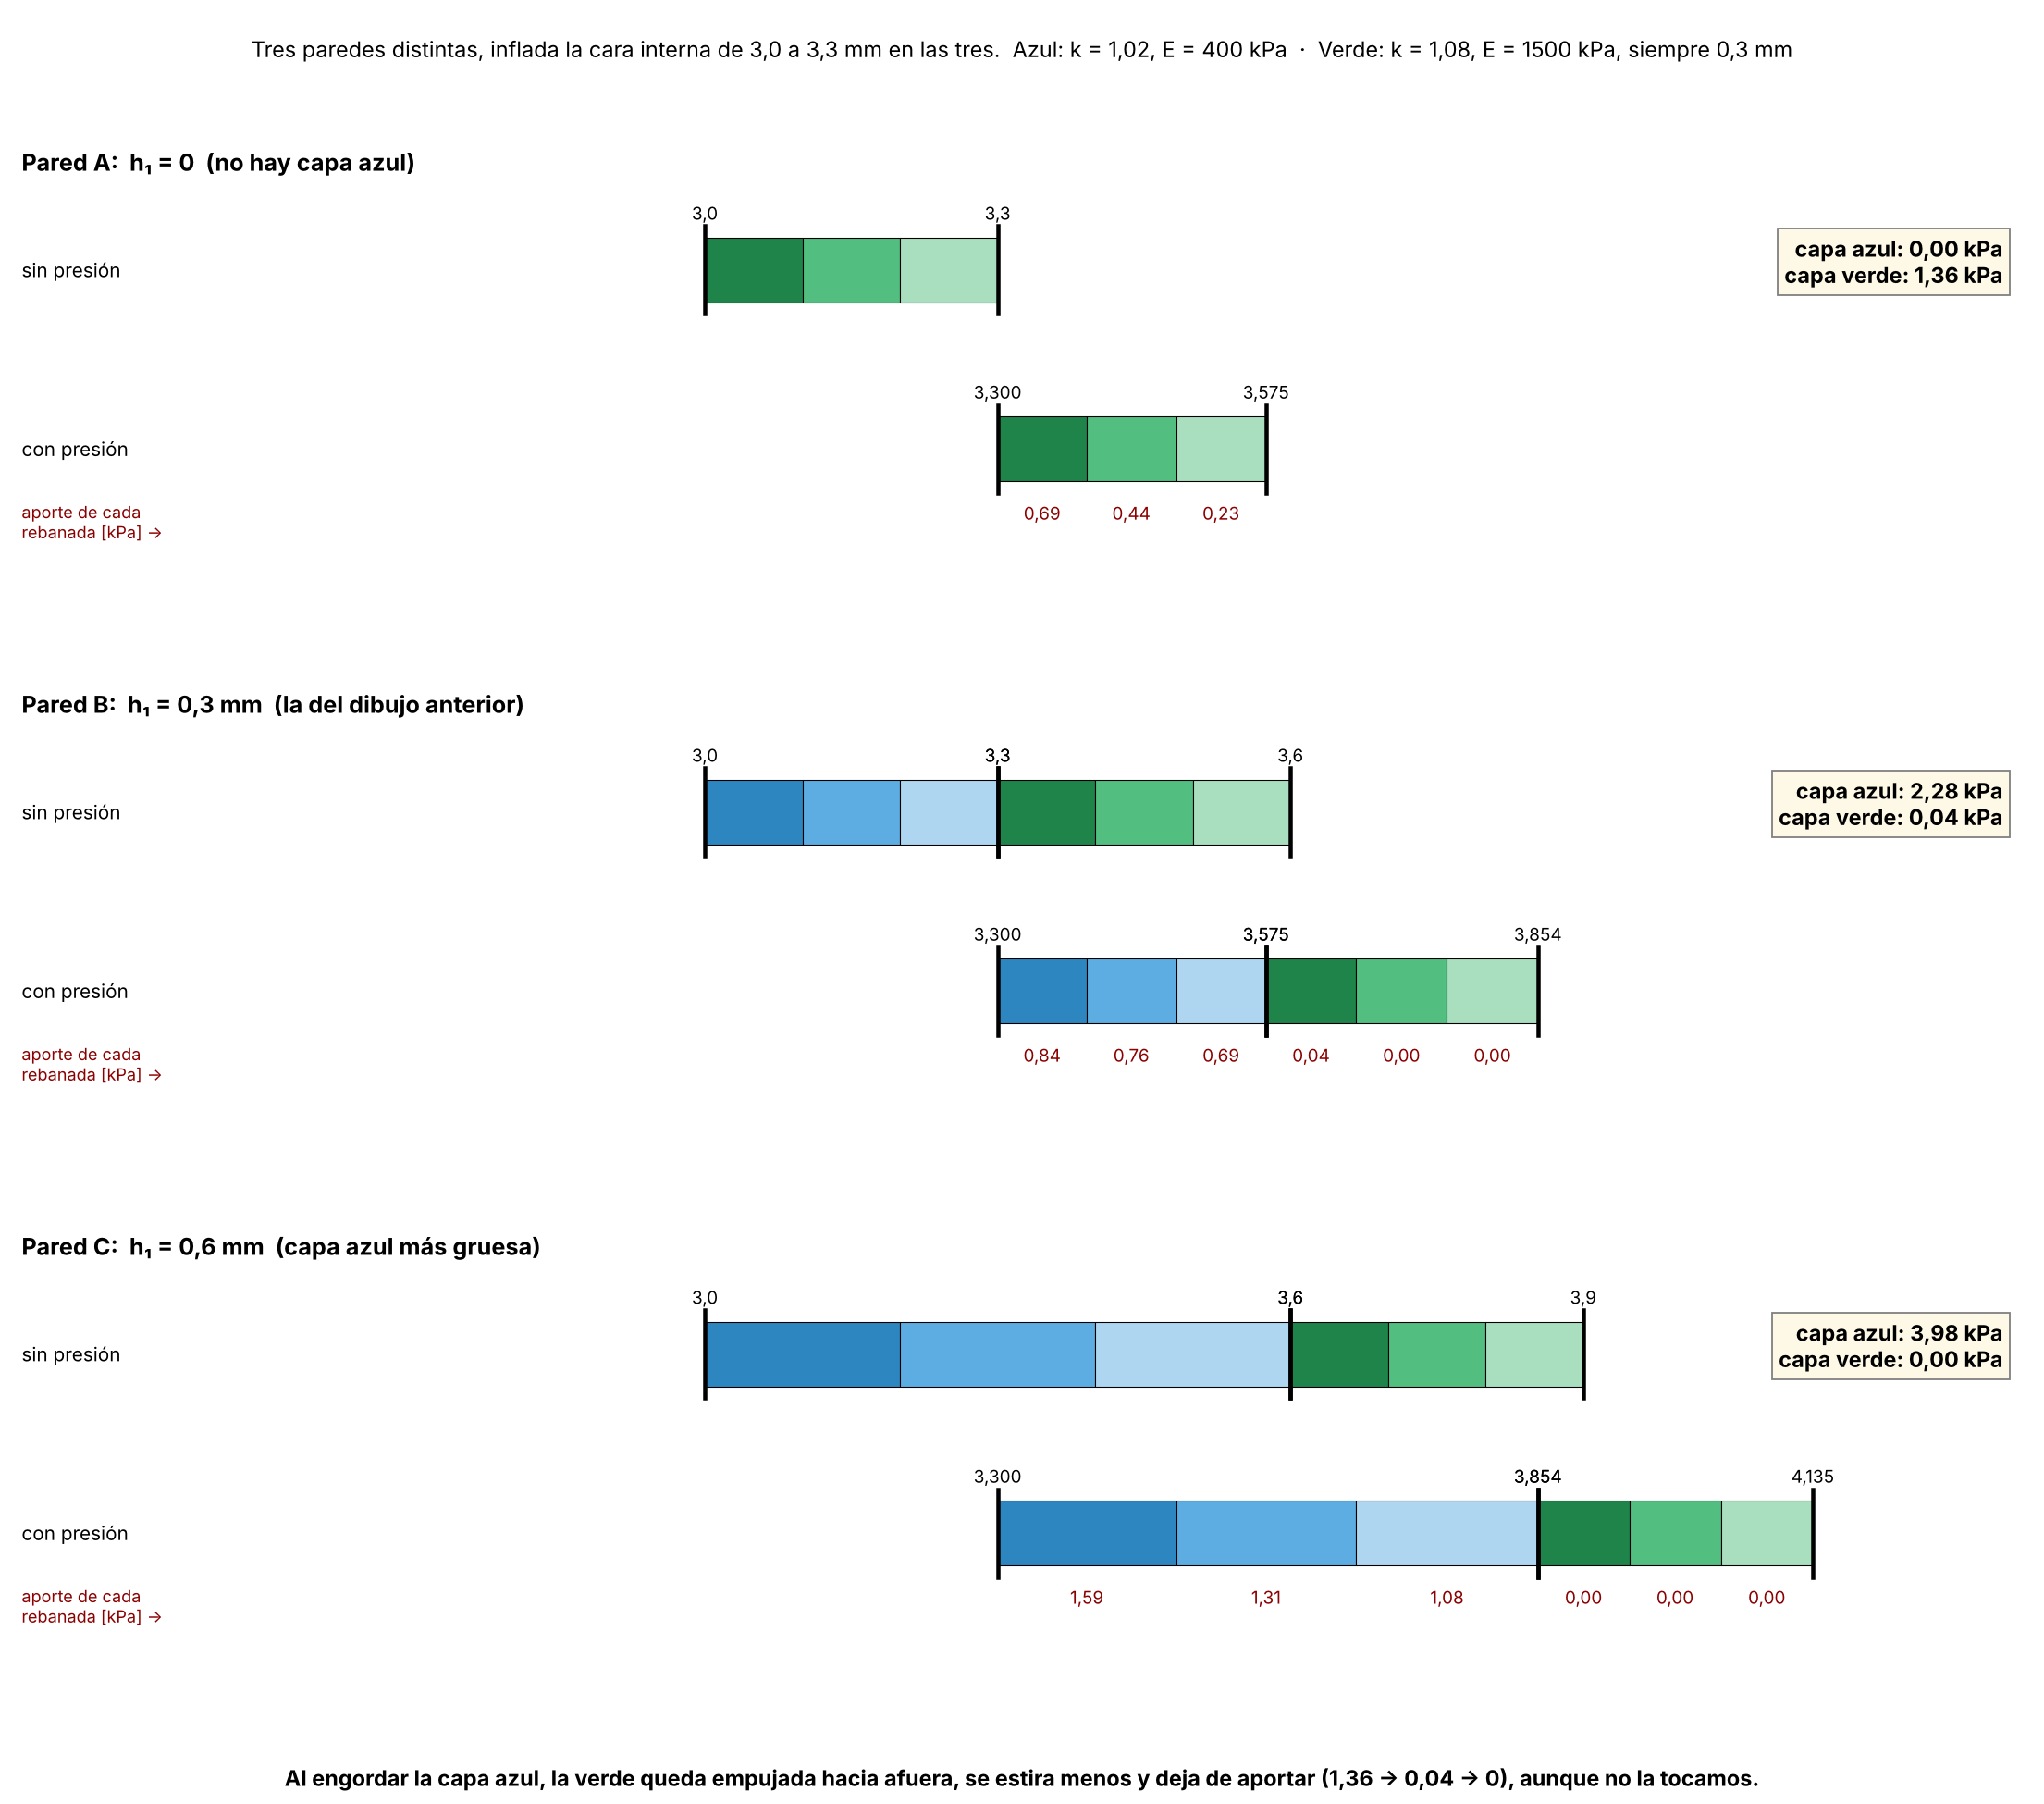
\includegraphics[width=\textwidth]{d17_tres_paredes.png}
\caption{Three walls with the same 0.3\,mm green layer and the same inner surface inflated to 3.3\,mm. Without a blue layer the green one contributes 1.36\,kPa; with 0.3\,mm of blue, 0.04; with 0.6\,mm, nothing. Doubling the blue layer raises its contribution from 2.28 to 3.98\,kPa, which is not twice as much: the problem is nonlinear in the thicknesses.}\end{figure}
\begin{figure}[H]\centering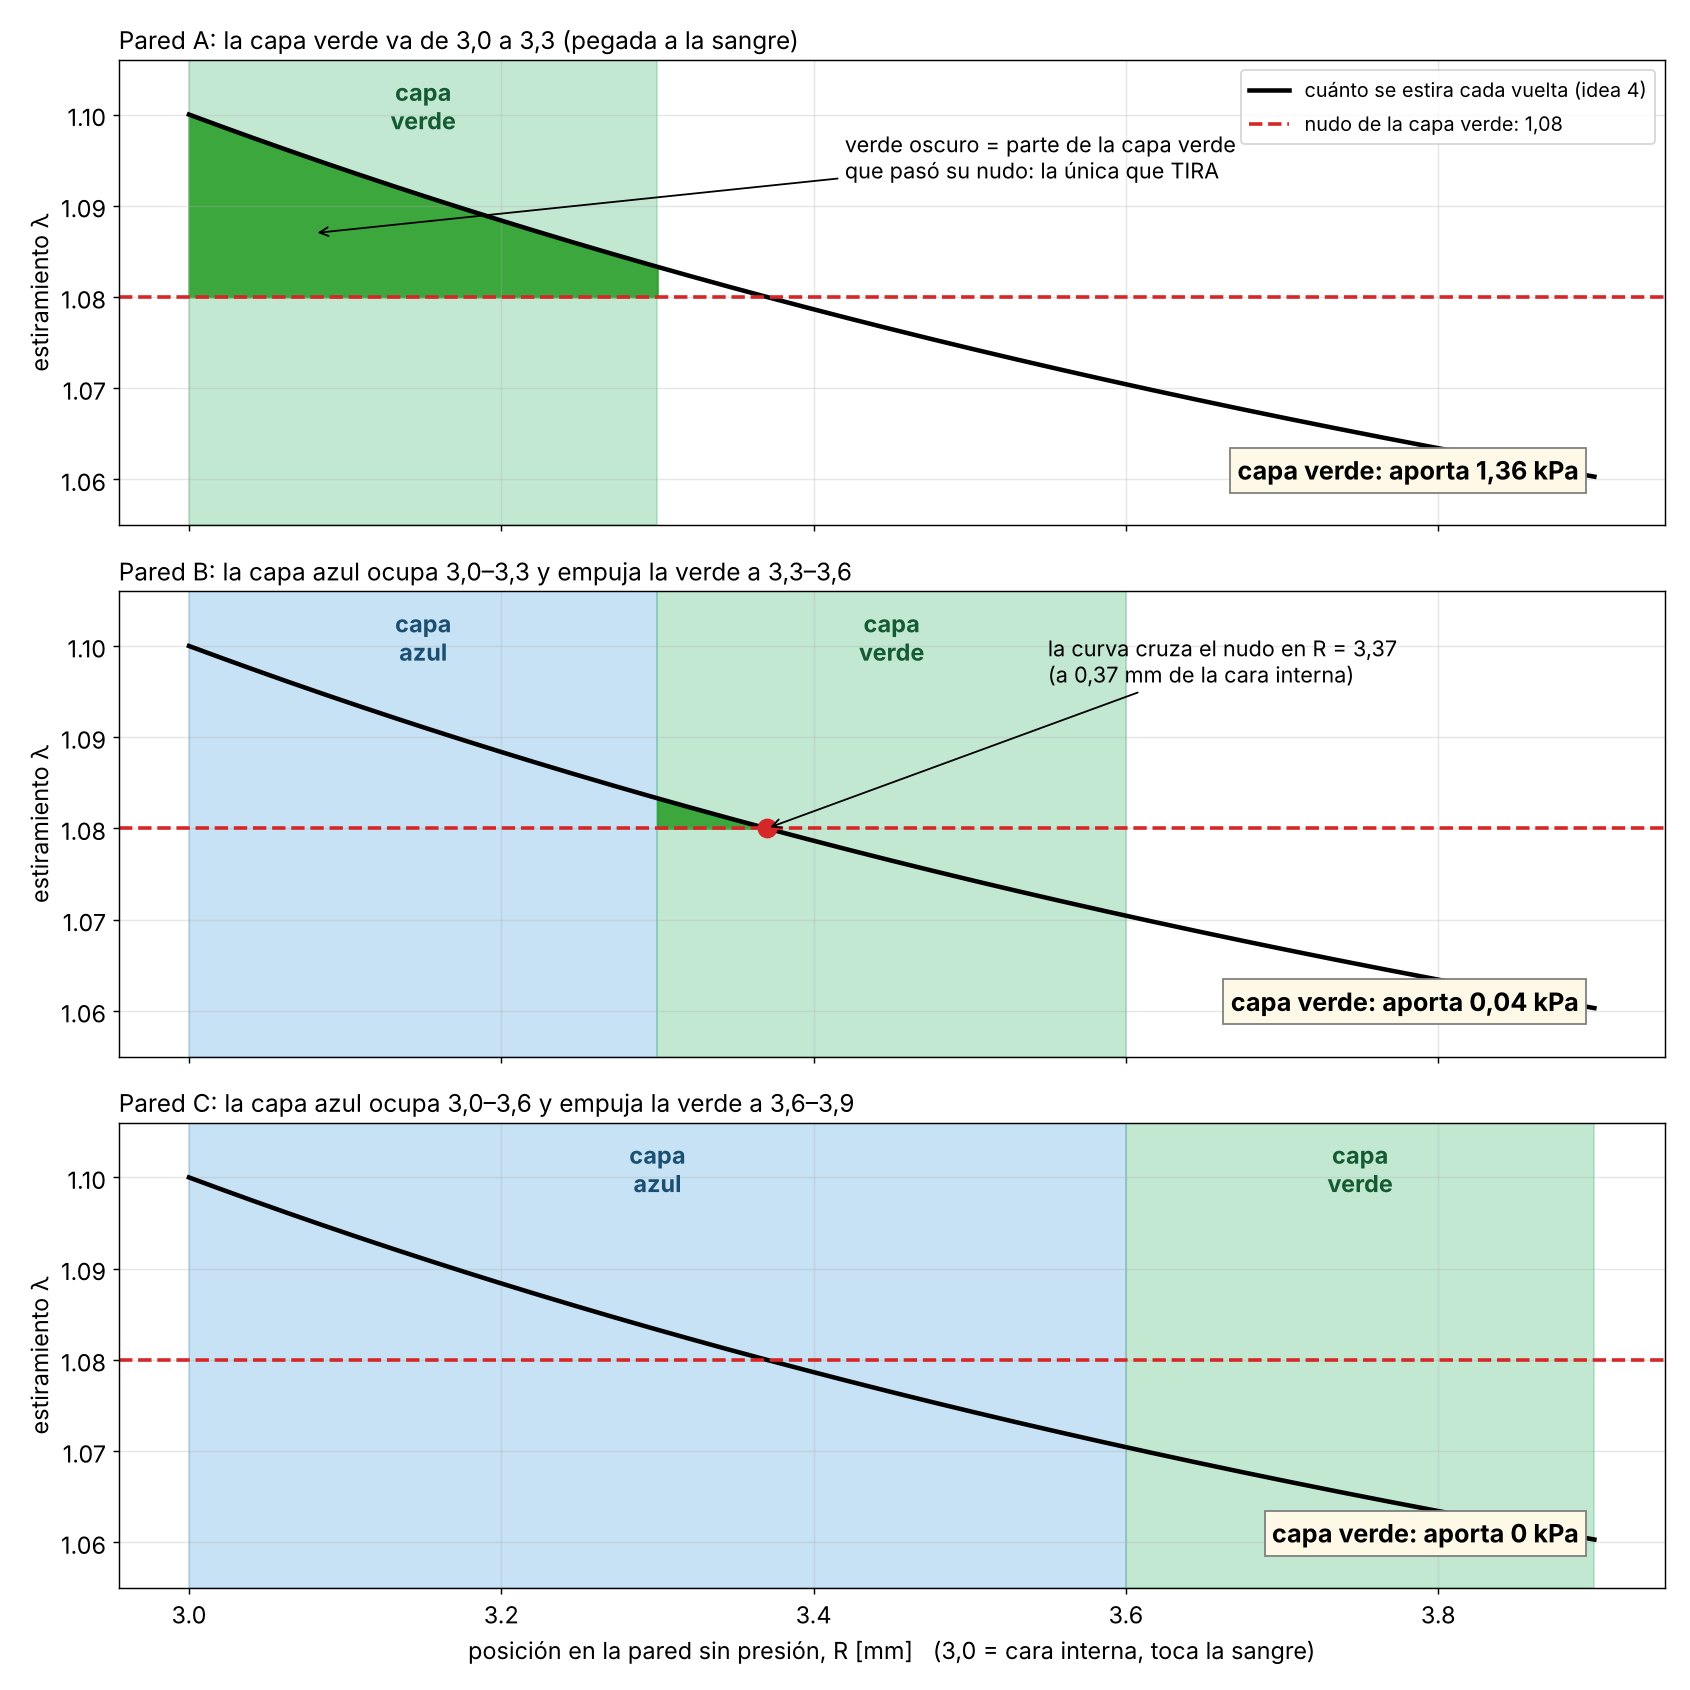
\includegraphics[width=0.85\textwidth]{d18_verde_y_nudo.png}
\caption{The same three walls seen as the stretch of each circumferential fiber versus its unpressurized radius (black curve) and the knot of the green layer (red line). The green layer contributes only in the part of it lying above 1.08 (dark green): in A, its whole inner part; in B, a sliver next to $R=3.37$\,mm; in C, nothing.}\end{figure}

\subsection{The prestretch $\delta$}
$\delta$ shifts all the knots together: the blue one moves to $1.02+\delta$ and the green one to $1.08+\delta$. The calculation for the two-layer wall (blue from 3.0 to 3.3, green from 3.3 to 3.6\,mm, inner surface inflated to 3.3\,mm) is repeated with three values of $\delta$. The stretches of the slices do not change (they depend only on the geometry); what changes is where each material starts bearing load.
\begin{center}\small
\begin{tabular}{lccccc}\toprule
 & & $\lambda$ & \multicolumn{3}{c}{$\sigma$ [kPa]}\\\cmidrule(lr){4-6}
Layer & center $R$ [mm] & & $\delta=-0.03$ & $\delta=0$ & $\delta=+0.03$\\\midrule
blue, $\sigma=400\max(0,\lambda-1.02-\delta)$ & 3.05 & 1.097 & 42.8 & 30.8 & 18.8\\
 & 3.15 & 1.091 & 40.4 & 28.4 & 16.4\\
 & 3.25 & 1.086 & 38.3 & 26.3 & 14.3\\
green, $\sigma=1500\max(0,\lambda-1.08-\delta)$ & 3.35 & 1.081 & 46.4 & 1.4 & 0\\
 & 3.45 & 1.076 & 39.7 & 0 & 0\\
 & 3.55 & 1.072 & 33.6 & 0 & 0\\\midrule
\multicolumn{3}{l}{contribution of the blue layer [kPa]} & 3.24 & 2.28 & 1.32\\
\multicolumn{3}{l}{contribution of the green layer [kPa]} & 3.00 & 0.04 & 0\\
\multicolumn{3}{l}{total pressure [kPa]} & 6.25 & 2.33 & 1.32\\\bottomrule
\end{tabular}
\end{center}
Verification example: first blue slice with $\delta=-0.03$: the knot is $1.02-0.03=0.99$ and $\sigma=400\times(1.097-0.99)=42.8$\,kPa; its contribution is $42.8\times0.091/3.346=1.16$\,kPa. With $\delta=-0.03$ the whole green layer passes its knot (1.05) and contributes as much as the blue one; with $\delta=+0.03$ the green knot rises to 1.11 and the green layer does not work. Thus, $\delta$ selects \emph{which materials are active} in the stretch interval of each subject: a soft subject, which stretches a lot, needs knots further to the right ($\delta>0$), and a stiff one, further to the left ($\delta<0$). Without $\delta$, each subject would see only one or two of the knots of the basis.
\begin{figure}[H]\centering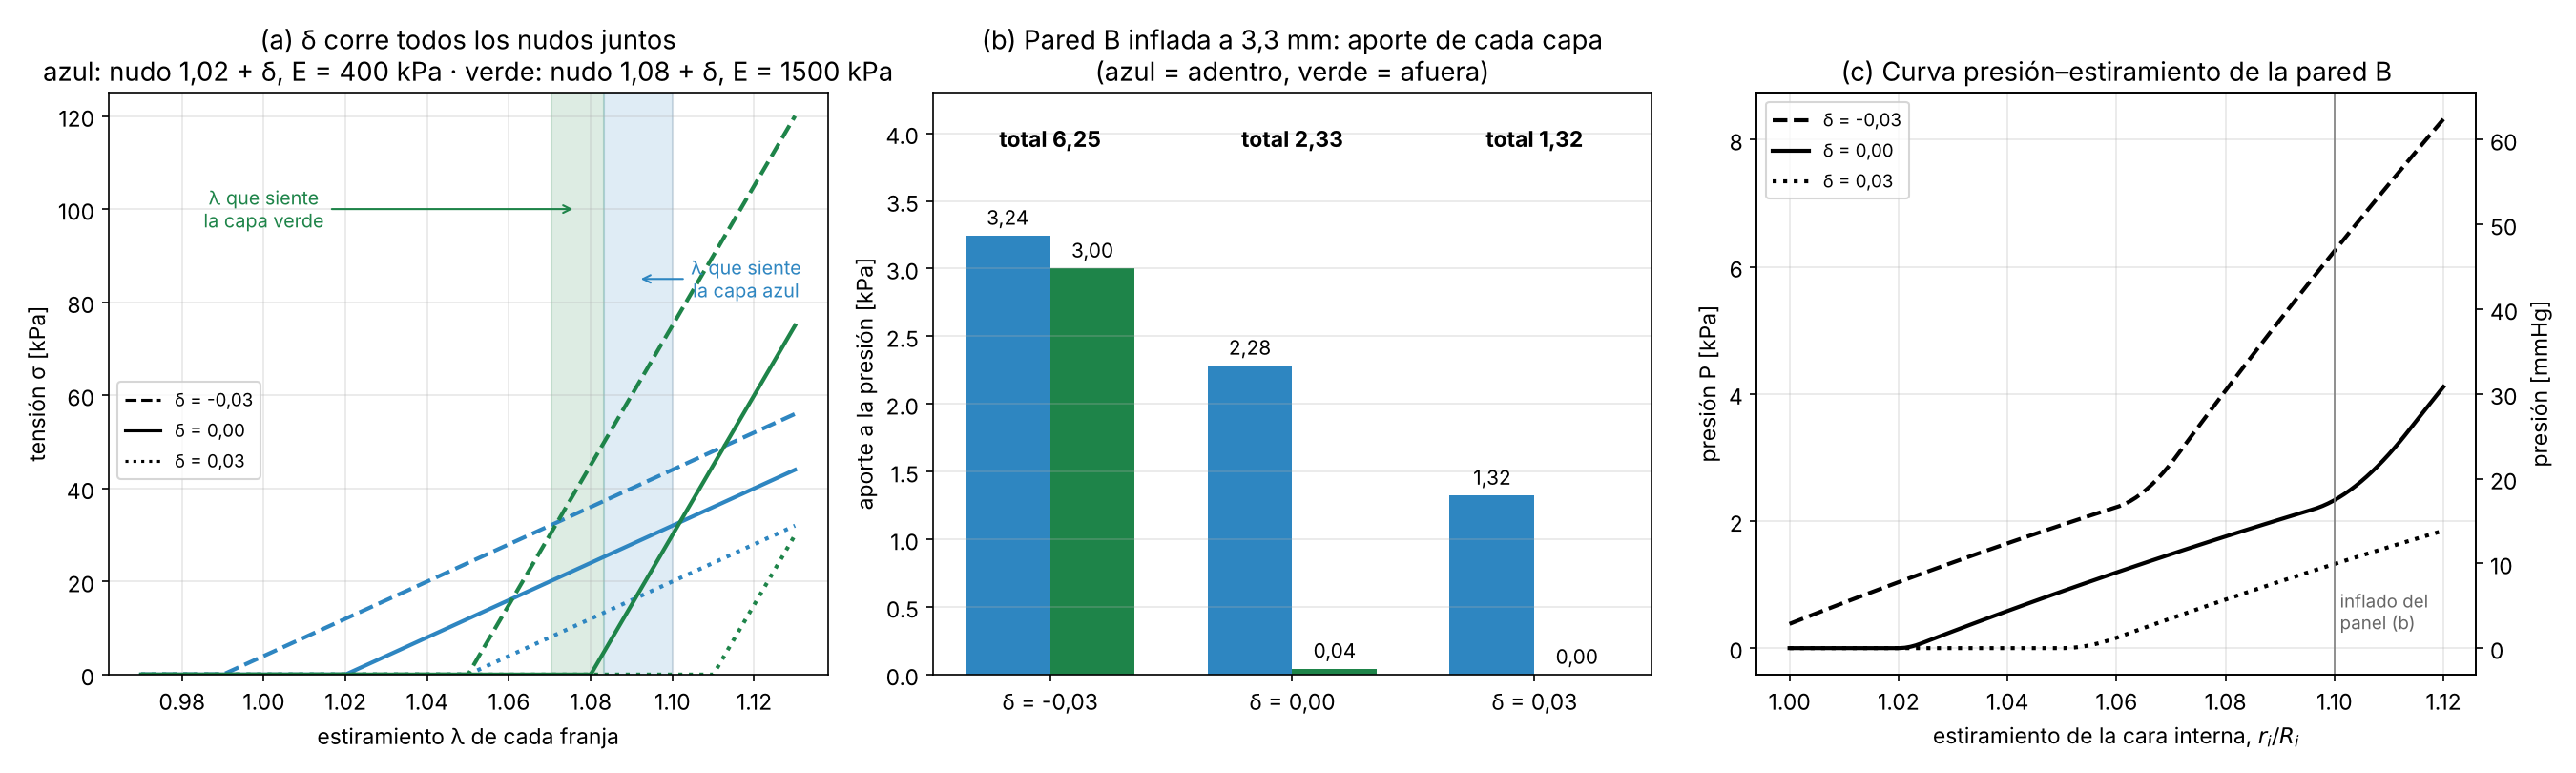
\includegraphics[width=\textwidth]{d19_delta.png}
\caption{Effect of $\delta$ on the two-layer wall. (a) Law of each material for $\delta=-0.03$, 0 and $+0.03$; the shaded bands are the stretches experienced by each layer with the inner surface at 3.3\,mm. (b) Contribution of each layer to the pressure in that state. (c) Pressure--stretch curve of the inner surface (right axis in mmHg): $\delta$ shifts the point at which each layer engages and changes the shape of the curve. The values belong to a toy example (0.3\,mm layers and low moduli), not to a design.}\end{figure}

\clearpage
\section{Training of the neural networks}\label{sec:entrenamiento}
Four networks were trained: the first-level network, which maps the curve $\sigma_{\theta\theta}(\lambda_\theta)$ to the amount of each material (Section~\ref{sec:validacion}), and the thick-wall network (block A4), each with 6 and with 5 materials. Fig.~\ref{fig:aprendizaje} shows the training and validation loss epoch by epoch, and Table~\ref{tab:entrenamiento} summarizes the training and the final loss on the three data sets. The test loss is computed on curves the network never saw, neither to fit the weights nor to decide when to stop.

\begin{figure}[H]\centering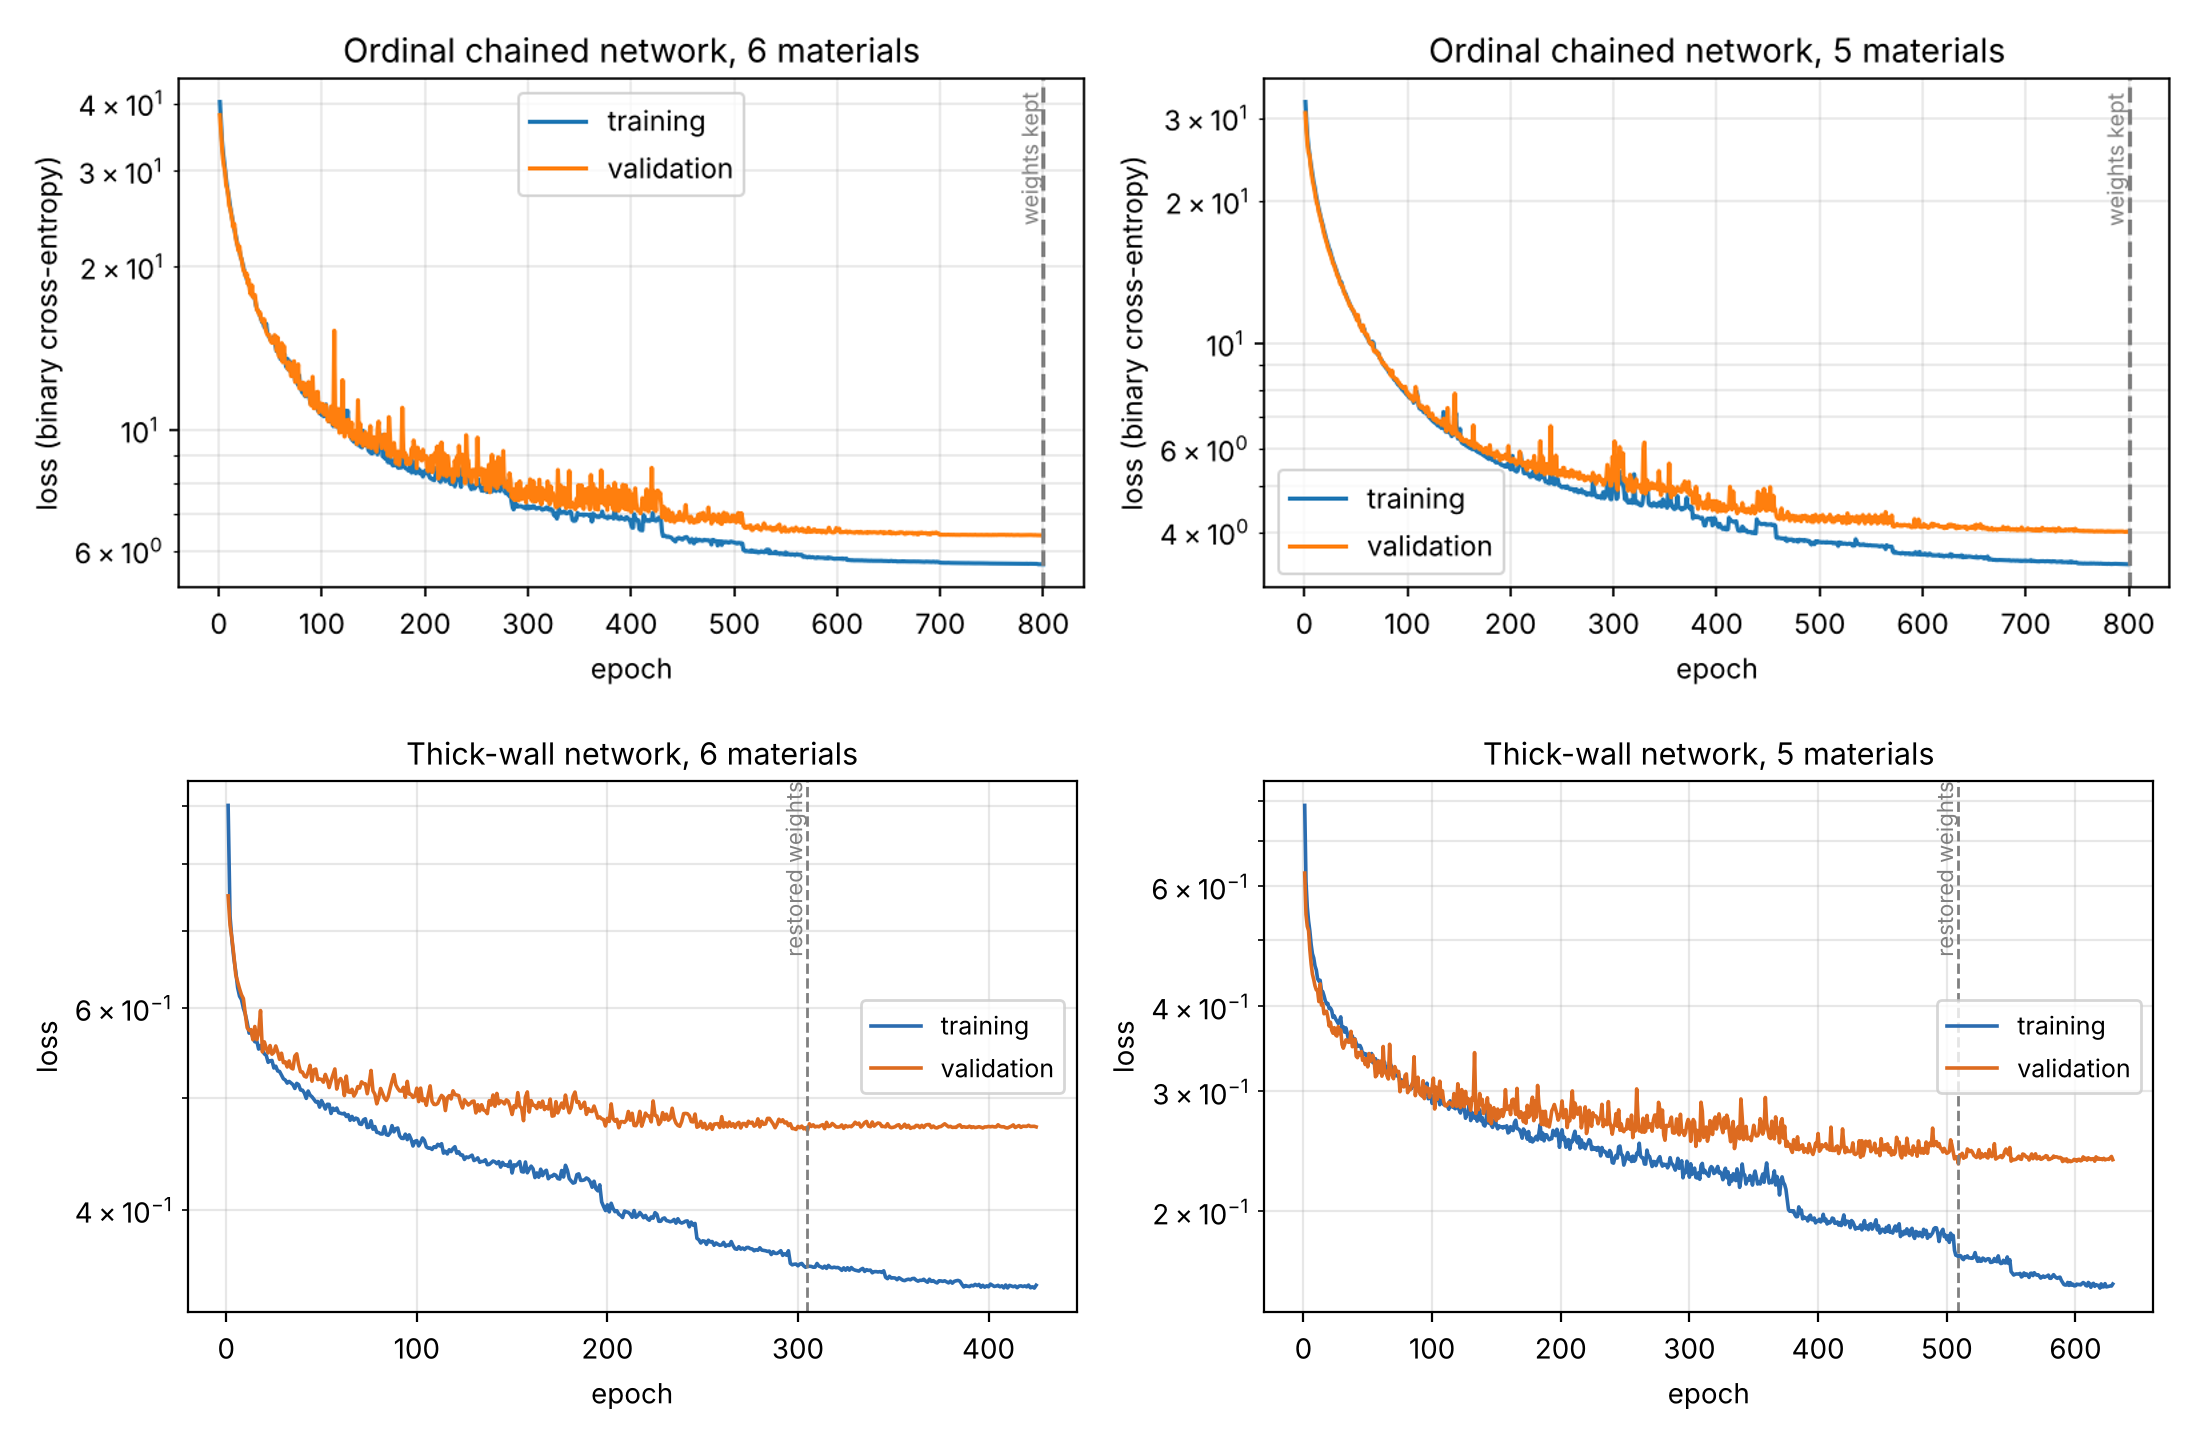
\includegraphics[width=\textwidth]{curvas_aprendizaje_en.png}
\caption{Learning curves: training (blue) and validation (orange) loss per epoch, on a logarithmic scale. The dashed line marks the epoch whose weights are kept. The loss logged during training includes the L2 regularization term. Top: first-level network (combined loss: amounts, curve and \emph{crosstalk}); bottom: thick-wall network (mean squared error of the standardized design).}\label{fig:aprendizaje}
\end{figure}

\begin{table}[H]\centering\small
\caption{Training summary. Epochs: total run and epoch whose weights are kept. Loss without the L2 term, computed with the kept weights and without noise added to the input; the first-level network uses the combined loss and the thick-wall network the mean squared error of the standardized design, so the two sets of values are not comparable with each other. The last column is the test loss divided by the training loss.}\label{tab:entrenamiento}
\resizebox{\textwidth}{!}{\begin{tabular}{llcccccc}\toprule
Network & Data (train/val/test) & Epochs & LR reductions & Train & Val. & Test & Test/train\\\midrule
$\sigma_{\theta\theta}$, 6 mat. & 35\,000 / 5000 / 10\,000 & 3000 / 2968 & 6 & $1.69\cdot10^{-4}$ & $2.28\cdot10^{-4}$ & $2.30\cdot10^{-4}$ & 1.36\\
$\sigma_{\theta\theta}$, 5 mat. & 35\,000 / 5000 / 10\,000 & 2439 / 2289 & 10 & $0.88\cdot10^{-4}$ & $1.08\cdot10^{-4}$ & $1.16\cdot10^{-4}$ & 1.31\\
Thick wall, 6 mat. & 11\,220 / 1530 / 2250 & 425 / 305 & 5 & 0.342 & 0.462 & 0.484 & 1.42\\
Thick wall, 5 mat. & 11\,220 / 1530 / 2250 & 629 / 509 & 4 & 0.153 & 0.227 & 0.250 & 1.64\\\bottomrule
\end{tabular}}
\end{table}

\paragraph{First-level network.} The training and validation curves decrease together and end almost on top of each other: the network does not memorize the data. The spikes are normal with small batches and fade as the learning rate is reduced. The 6-material network reached the limit of 3000 epochs with the loss already stable (within 1\,\% of its minimum from epoch 2943 on); the 5-material network was stopped by early stopping. The test loss is only slightly above the validation loss. In standardized units, the mean absolute error of each amount on the test set is 0.0072 (6 materials) and 0.0051 (5), about 0.02 laminae. Measured on the curve, the NRMSE of the network exceeds that of the exact least-squares fit by less than 3.2\,\% (relative) in the physiological test families (Table~\ref{tab:familias}).

\paragraph{Thick-wall network.} Here validation departs from training within the first 50 epochs and levels off, while the training loss keeps decreasing. Early stopping keeps the weights at the validation minimum, and the test loss stays close to the validation loss (0.484 vs.\ 0.462 and 0.250 vs.\ 0.227): the network does not degrade on new data. The loss is nevertheless high, and the reason lies in the problem, not in the network: the thick-wall inverse problem (from the curve to the design) is ill-conditioned.

\emph{Conditioning.} For 60 arteries from the physiological families, the Jacobian $J$ of the graft curve with respect to the design $\theta=(h_1\ldots h_N,\delta)$ was computed by finite differences, with each parameter measured in standard deviations (the scale used by the network) and the curve in \% of its range. Its singular values tell how much the curve moves when the design moves in each direction. With 6 materials, in the most sensitive direction the curve changes by about 850\,\% of its range per standard deviation (8.5 times the range); in the least sensitive one, by only 1\,\% (with 5 materials: 750\,\% and 2.6\,\%). The condition number $\kappa(J)$ has a median of 900 with 6 materials and 300 with 5 (90th percentile: $2.4\cdot10^{4}$ and $1.5\cdot10^{4}$), compared with $\mathrm{cond}(A)=28$ at the first level. The least sensitive direction is typically more thickness of one material and less of its neighbor: it changes the design by one standard deviation and the curve by 1\,\%, the same order as the 0 to 1\,\% noise used to train the network. From the curve, such designs are indistinguishable for any method, and the network cannot guess which one is the label. This explains the high loss, and why 5 materials, which is better conditioned, has half the loss of 6.

\emph{The measure that matters.} For the graft, two designs whose curves differ by less than 1\,\% are equally good; ill-conditioning means that there are many acceptable designs, not that the design is uncertain. The network is therefore judged by the curve error, which is the design criterion. Over 500 test curves, the curve of the design proposed by the network has a median worst-point error of 6.1\,\% of the range with 6 materials and 4.3\,\% with 5: 3 to 4\,\% for arteries and 11 to 12\,\% for grafts with random designs, which cover the whole design space. That is not enough to design with, and the network is not used that way: it is the starting point of the A2 fit, which brings the design to the target (Section~\ref{sec:aplicacion}). A network trained with a loss on the curve, like the first-level network, would reduce that starting error.

\begin{thebibliography}{99}\small
\bibitem{aarts} Aarts, E., Lenstra, J.\,K. (eds.) (1997). \emph{Local Search in Combinatorial Optimization}. Wiley.
\bibitem{tf} Abadi, M., et al. (2016). TensorFlow: a system for large-scale machine learning. \emph{Proc. 12th USENIX OSDI}, 265--283.
\bibitem{agrell} Agrell, E., Eriksson, T., Vardy, A., Zeger, K. (2002). Closest point search in lattices. \emph{IEEE Trans. Inf. Theory} 48(8), 2201--2214.
\bibitem{amos} Amos, B. (2023). Tutorial on amortized optimization. \emph{Found. Trends Mach. Learn.} 16(5), 592--732.
\bibitem{layernorm} Ba, J.\,L., Kiros, J.\,R., Hinton, G.\,E. (2016). Layer normalization. arXiv:1607.06450.
\bibitem{branch} Branch, M.\,A., Coleman, T.\,F., Li, Y. (1999). A subspace, interior, and conjugate gradient method for large-scale bound-constrained minimization problems. \emph{SIAM J. Sci. Comput.} 21(1), 1--23.
\bibitem{brent} Brent, R.\,P. (1973). \emph{Algorithms for Minimization without Derivatives}. Prentice-Hall.
\bibitem{cheney} Cheney, E.\,W. (1966). \emph{Introduction to Approximation Theory}. McGraw-Hill.
\bibitem{davis} Davis, P.\,J., Rabinowitz, P. (1984). \emph{Methods of Numerical Integration}, 2nd ed. Academic Press.
\bibitem{ding} Ding, X., Sha, D., Sun, K., Fan, Y. (2025). Biomechanical insights into the development and optimization of small-diameter vascular grafts. \emph{Acta Biomater.} doi:10.1016/j.actbio.2025.04.028.
\bibitem{engelen13} Engelen, L., Ferreira, I., Stehouwer, C.\,D.\,A., Boutouyrie, P., Laurent, S.; Reference Values for Arterial Measurements Collaboration (2013). Reference intervals for common carotid intima-media thickness measured with echotracking: relation with risk factors. \emph{Eur. Heart J.} 34(30), 2368--2380.
\bibitem{pchip} Fritsch, F.\,N., Carlson, R.\,E. (1980). Monotone piecewise cubic interpolation. \emph{SIAM J. Numer. Anal.} 17(2), 238--246.
\bibitem{fung} Fung, Y.\,C. (1993). \emph{Biomechanics: Mechanical Properties of Living Tissues}, 2nd ed. Springer.
\bibitem{furdella} Furdella, K.\,J., Higuchi, S., Behrangzade, A., Kim, K., Wagner, W.\,R., Vande Geest, J.\,P. (2021). In-vivo assessment of a tissue engineered vascular graft computationally optimized for target vessel compliance. \emph{Acta Biomater.} 123, 298--311.
\bibitem{golub} Golub, G.\,H., Van Loan, C.\,F. (2013). \emph{Matrix Computations}, 4th ed. Johns Hopkins University Press.
\bibitem{goodfellow} Goodfellow, I., Bengio, Y., Courville, A. (2016). \emph{Deep Learning}. MIT Press.
\bibitem{numpy} Harris, C.\,R., et al. (2020). Array programming with NumPy. \emph{Nature} 585, 357--362.
\bibitem{harrison} Harrison, S., Tamimi, E., Uhlorn, J., Leach, T., Vande Geest, J.\,P. (2016). Computationally optimizing the compliance of a biopolymer based tissue engineered vascular graft. \emph{J. Biomech. Eng.} 138(1), 014505.
\bibitem{holzapfel} Holzapfel, G.\,A., Gasser, T.\,C., Ogden, R.\,W. (2000). A new constitutive framework for arterial wall mechanics and a comparative study of material models. \emph{J. Elasticity} 61, 1--48.
\bibitem{hsu} Hsu, R., Szafron, J.\,M., Carvalho, C.\,C., Humphrey, J.\,D., Marsden, A.\,L. (2025). Constrained optimization of scaffold behavior for improving tissue engineered vascular grafts. \emph{J. Biomech.} doi:10.1016/j.jbiomech.2025.112670.
\bibitem{highs} Huangfu, Q., Hall, J.\,A.\,J. (2018). Parallelizing the dual revised simplex method. \emph{Math. Program. Comput.} 10, 119--142.
\bibitem{humphrey} Humphrey, J.\,D. (2002). \emph{Cardiovascular Solid Mechanics: Cells, Tissues, and Organs}. Springer.
\bibitem{jiang} Jiang, D., Robinson, A.\,J., Nkansah, A., et al. (2025). A computational framework to optimize the mechanical behavior of synthetic vascular grafts. \emph{J. Mech. Behav. Biomed. Mater.} 163, 106847.
\bibitem{kamenskiy} Kamenskiy, A.\,V., Dzenis, Y.\,A., MacTaggart, J.\,N., Lynch, T.\,G., Jaffar Kazmi, S.\,A., Pipinos, I.\,I. (2012). Nonlinear mechanical behavior of the human common, external, and internal carotid arteries in vivo. \emph{J. Surg. Res.}
\bibitem{adam} Kingma, D.\,P., Ba, J. (2015). Adam: a method for stochastic optimization. \emph{Proc. ICLR}.
\bibitem{lawson} Lawson, C.\,L., Hanson, R.\,J. (1995). \emph{Solving Least Squares Problems}. SIAM.
\bibitem{liu} Liu, H., et al. (2012). Using in vivo Cine and 3D multi-contrast MRI to determine human atherosclerotic carotid artery material properties and circumferential shrinkage rate and their impact on stress/strain predictions. \emph{J. Biomech. Eng.} 134, 011008.
\bibitem{masson} Masson, I., Beaussier, H., Boutouyrie, P., Laurent, S., Humphrey, J.\,D., Zidi, M. (2011). Carotid artery mechanical properties and stresses quantified using in vivo data from normotensive and hypertensive humans. \emph{Biomech. Model. Mechanobiol.} 10(6), 867--882.
\bibitem{relu} Nair, V., Hinton, G.\,E. (2010). Rectified linear units improve restricted Boltzmann machines. \emph{Proc. ICML}.
\bibitem{nelder} Nelder, J.\,A., Mead, R. (1965). A simplex method for function minimization. \emph{Computer J.} 7(4), 308--313.
\bibitem{penrose} Penrose, R. (1955). A generalized inverse for matrices. \emph{Math. Proc. Cambridge Philos. Soc.} 51(3), 406--413.
\bibitem{prechelt} Prechelt, L. (1998). Early stopping --- but when? In \emph{Neural Networks: Tricks of the Trade}, LNCS 1524, 55--69.
\bibitem{rachev} Rachev, A., Hayashi, K. (1999). Theoretical study of the effects of vascular smooth muscle contraction on strain and stress distributions in arteries. \emph{Ann. Biomed. Eng.} 27, 459--468.
\bibitem{rockafellar} Rockafellar, R.\,T., Uryasev, S. (2000). Optimization of conditional value-at-risk. \emph{J. Risk} 2(3), 21--41.
\bibitem{rovas23} Rovas, G., Bikia, V., Stergiopulos, N. (2023). Design and computational optimization of compliance-matching aortic grafts. \emph{Front. Bioeng. Biotechnol.} 11, 1179174.
\bibitem{rovas25} Rovas, G., Reymond, P., van Steenberghe, M., et al., Stergiopulos, N. (2025). Evaluation of a novel compliance-matching aortic graft in a swine model. \emph{J. Biomech.} doi:10.1016/j.jbiomech.2025.112629.
\bibitem{sommer} Sommer, G., Holzapfel, G.\,A. (2012). 3D constitutive modeling of the biaxial mechanical response of intact and layer-dissected human carotid arteries. \emph{J. Mech. Behav. Biomed. Mater.} 5, 116--128.
\bibitem{storn} Storn, R., Price, K. (1997). Differential evolution: a simple and efficient heuristic for global optimization over continuous spaces. \emph{J. Global Optim.} 11, 341--359.
\bibitem{szafron} Szafron, J.\,M., Ramachandra, A.\,B., Breuer, C.\,K., Marsden, A.\,L., Humphrey, J.\,D. (2019). Optimization of tissue-engineered vascular graft design using computational modeling. \emph{Tissue Eng. Part C}. doi:10.1089/ten.tec.2019.0086.
\bibitem{tamimi} Tamimi, E.\,A., Ardila, D.\,C., Ensley, B.\,D., Kellar, R.\,S., Vande Geest, J.\,P. (2019). Computationally optimizing the compliance of multilayered biomimetic tissue engineered vascular grafts. \emph{J. Biomech. Eng.} doi:10.1115/1.4042902.
\bibitem{trefethen} Trefethen, L.\,N., Bau, D. (1997). \emph{Numerical Linear Algebra}. SIAM.
\bibitem{urquiza} Urquiza, S.\,A. (2009). \emph{Hemodinámica computacional del sistema arterial humano} [Computational hemodynamics of the human arterial system]. Doctoral thesis in Engineering Sciences, Instituto Balseiro, Universidad Nacional de Cuyo, San Carlos de Bariloche, Argentina (in Spanish). Ch.~3, Eq.~(3.13).
\bibitem{scipy} Virtanen, P., et al. (2020). SciPy 1.0: fundamental algorithms for scientific computing in Python. \emph{Nat. Methods} 17, 261--272.
\end{thebibliography}
\end{document}
